% Options for packages loaded elsewhere
\PassOptionsToPackage{unicode}{hyperref}
\PassOptionsToPackage{hyphens}{url}
%
\documentclass[
]{article}
\usepackage{amsmath,amssymb}
\usepackage{iftex}
\ifPDFTeX
  \usepackage[T1]{fontenc}
  \usepackage[utf8]{inputenc}
  \usepackage{textcomp} % provide euro and other symbols
\else % if luatex or xetex
  \usepackage{unicode-math} % this also loads fontspec
  \defaultfontfeatures{Scale=MatchLowercase}
  \defaultfontfeatures[\rmfamily]{Ligatures=TeX,Scale=1}
\fi
\usepackage{lmodern}
\ifPDFTeX\else
  % xetex/luatex font selection
\fi
% Use upquote if available, for straight quotes in verbatim environments
\IfFileExists{upquote.sty}{\usepackage{upquote}}{}
\IfFileExists{microtype.sty}{% use microtype if available
  \usepackage[]{microtype}
  \UseMicrotypeSet[protrusion]{basicmath} % disable protrusion for tt fonts
}{}
\makeatletter
\@ifundefined{KOMAClassName}{% if non-KOMA class
  \IfFileExists{parskip.sty}{%
    \usepackage{parskip}
  }{% else
    \setlength{\parindent}{0pt}
    \setlength{\parskip}{6pt plus 2pt minus 1pt}}
}{% if KOMA class
  \KOMAoptions{parskip=half}}
\makeatother
\usepackage{xcolor}
\usepackage[margin=1in]{geometry}
\usepackage{graphicx}
\makeatletter
\def\maxwidth{\ifdim\Gin@nat@width>\linewidth\linewidth\else\Gin@nat@width\fi}
\def\maxheight{\ifdim\Gin@nat@height>\textheight\textheight\else\Gin@nat@height\fi}
\makeatother
% Scale images if necessary, so that they will not overflow the page
% margins by default, and it is still possible to overwrite the defaults
% using explicit options in \includegraphics[width, height, ...]{}
\setkeys{Gin}{width=\maxwidth,height=\maxheight,keepaspectratio}
% Set default figure placement to htbp
\makeatletter
\def\fps@figure{htbp}
\makeatother
\setlength{\emergencystretch}{3em} % prevent overfull lines
\providecommand{\tightlist}{%
  \setlength{\itemsep}{0pt}\setlength{\parskip}{0pt}}
\setcounter{secnumdepth}{-\maxdimen} % remove section numbering
\ifLuaTeX
  \usepackage{selnolig}  % disable illegal ligatures
\fi
\usepackage{bookmark}
\IfFileExists{xurl.sty}{\usepackage{xurl}}{} % add URL line breaks if available
\urlstyle{same}
\hypersetup{
  pdftitle={Supplemental Information 1},
  hidelinks,
  pdfcreator={LaTeX via pandoc}}

\title{Supplemental Information 1}
\author{}
\date{\vspace{-2.5em}}

\begin{document}
\maketitle

\subsection{Description}\label{description}

Interval mapping (IM) and multiple-quantitative-trait-locus mapping
(MQM) scans for heading date (HD) and plant height (PH), Fusarium head
blight (FHB) visual ratings (VR), Fusarium damaged kernels (FDK), and
deoxynivalenol (DON) content quantitative trait loci (QTL). Presented
are the results of scans performed without heading date and plant height
marker covariates. In the title of each graph is displayed which type of
scan (IM vs MQM) and the trait which the scan belongs to. The number
following MQM titles indicates which round of MQM the scan belongs to
(e.g., MQM 2 is the second round of multiple QTL mapping). The y-axis
displays the likelihood of odds (LOD) score of every position across the
genome. The dotted line denotes the 1000 permutation significance
threshold at alpha equals 0.05. If the significance threshold is not
displayed within the graph, this indicates that all peaks detected in
the QTL scan were below the significance threshold. This is usually
apparent in the last MQM scan performed. The x-axis displays each
linkage group, designated by their corresponding chromosome names (e.g.,
1A, 1B, 1D, etc.). The rug of hash marks denotes the cM position of each
marker in the recombination map.

\subsection{Visual Ratings Across All
Environments}\label{visual-ratings-across-all-environments}

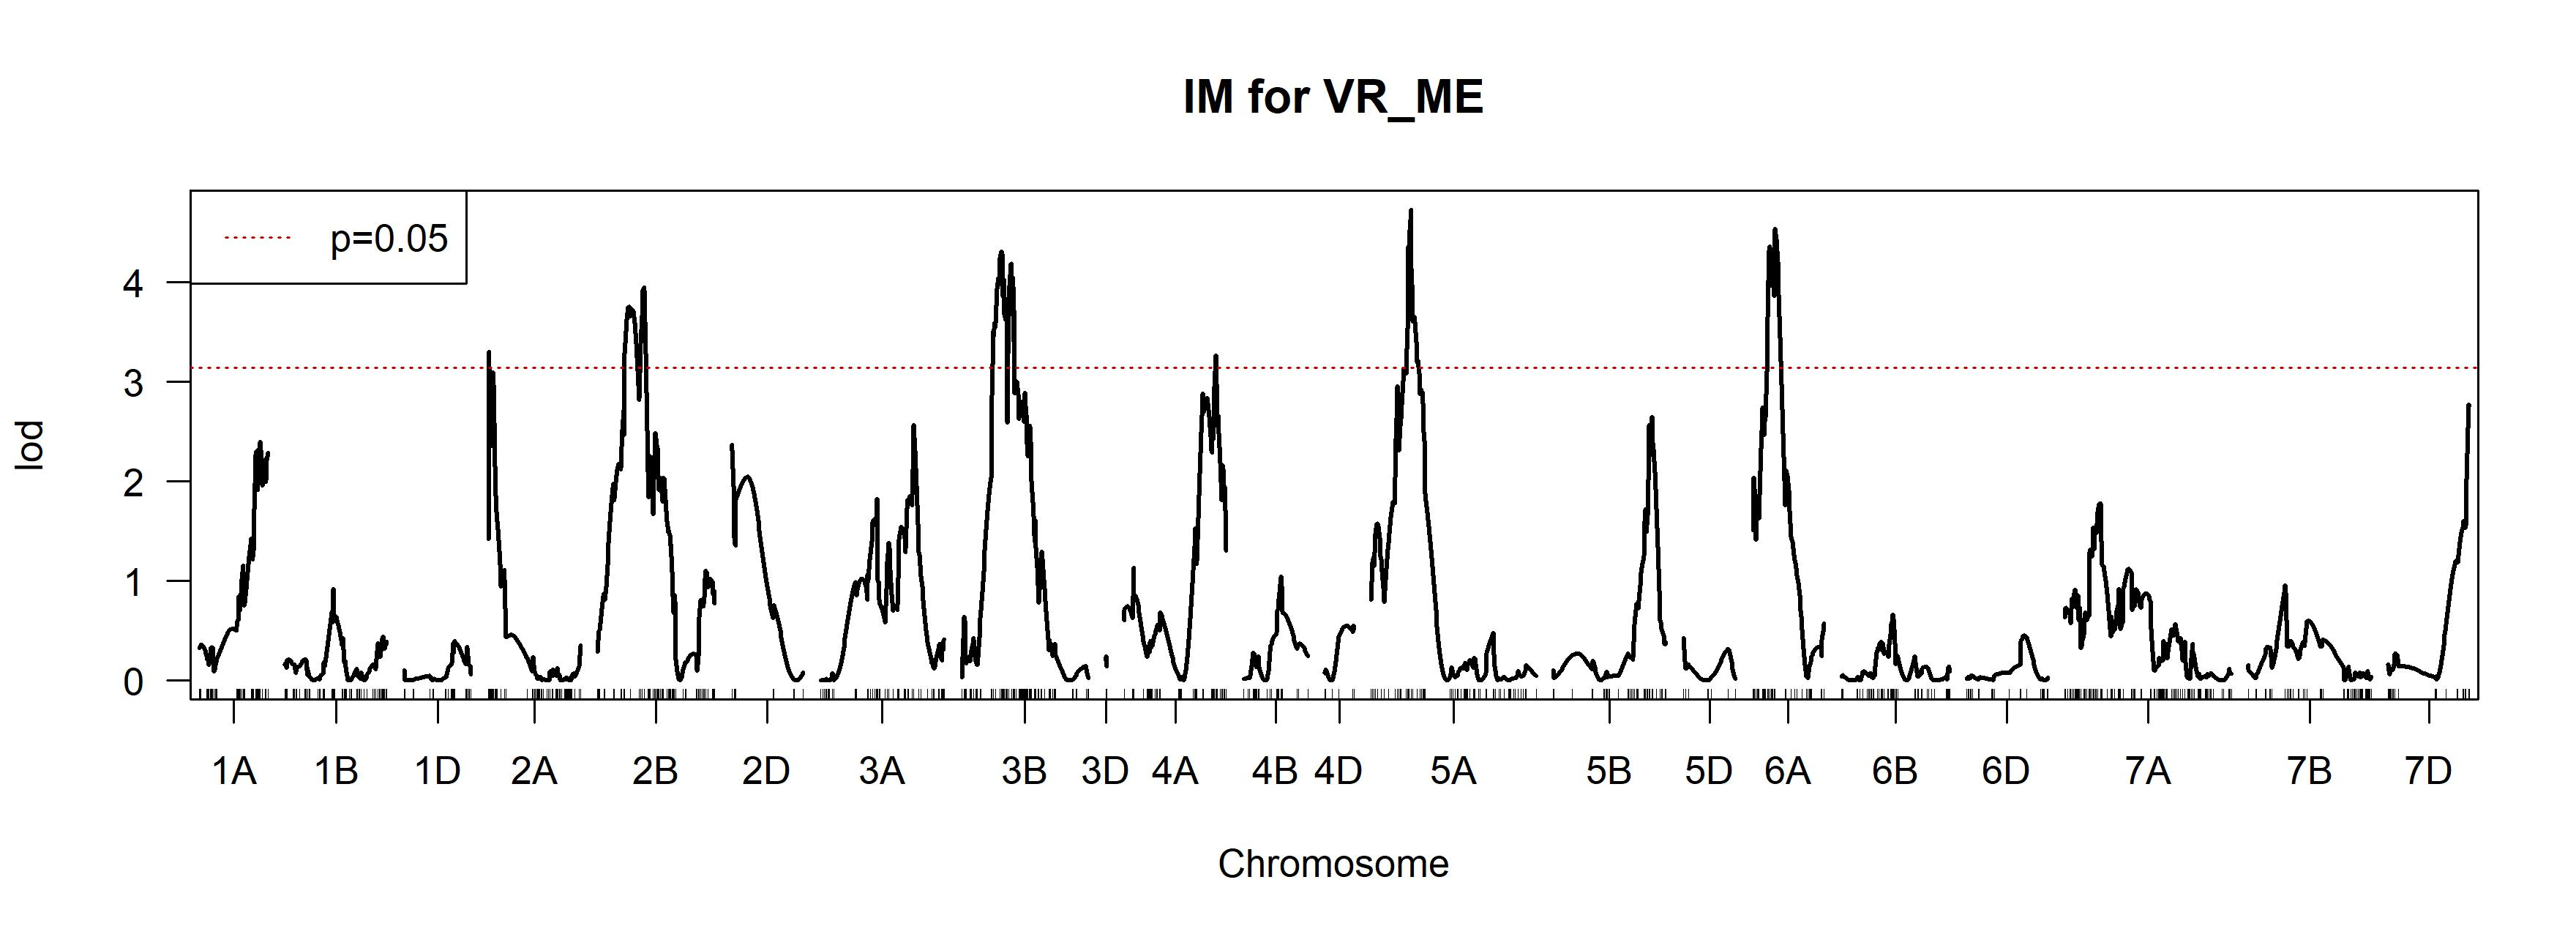
\includegraphics{Scan_IM_VR_ME.jpg}
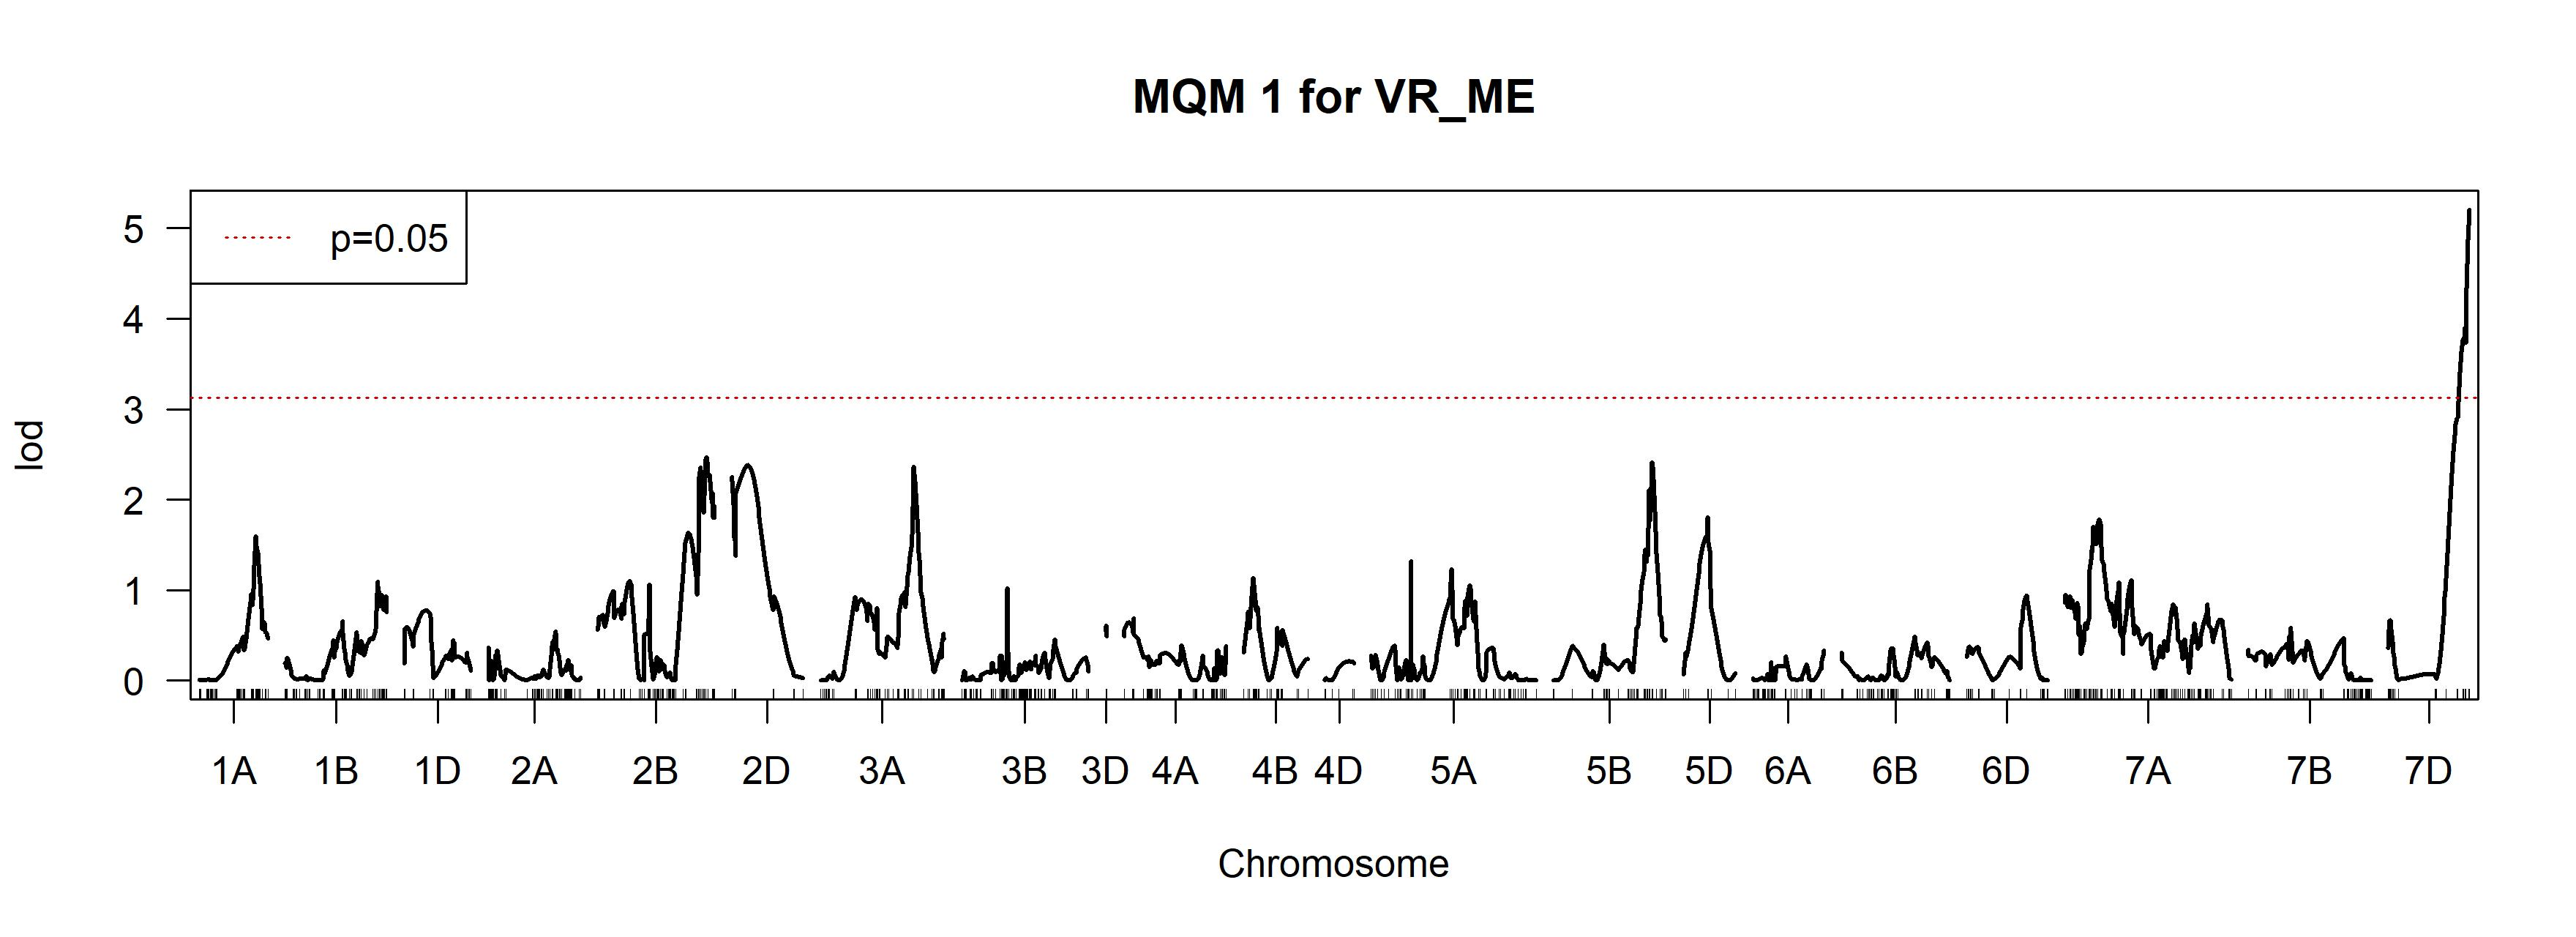
\includegraphics{Scan_MQM1_VR_ME.jpg}
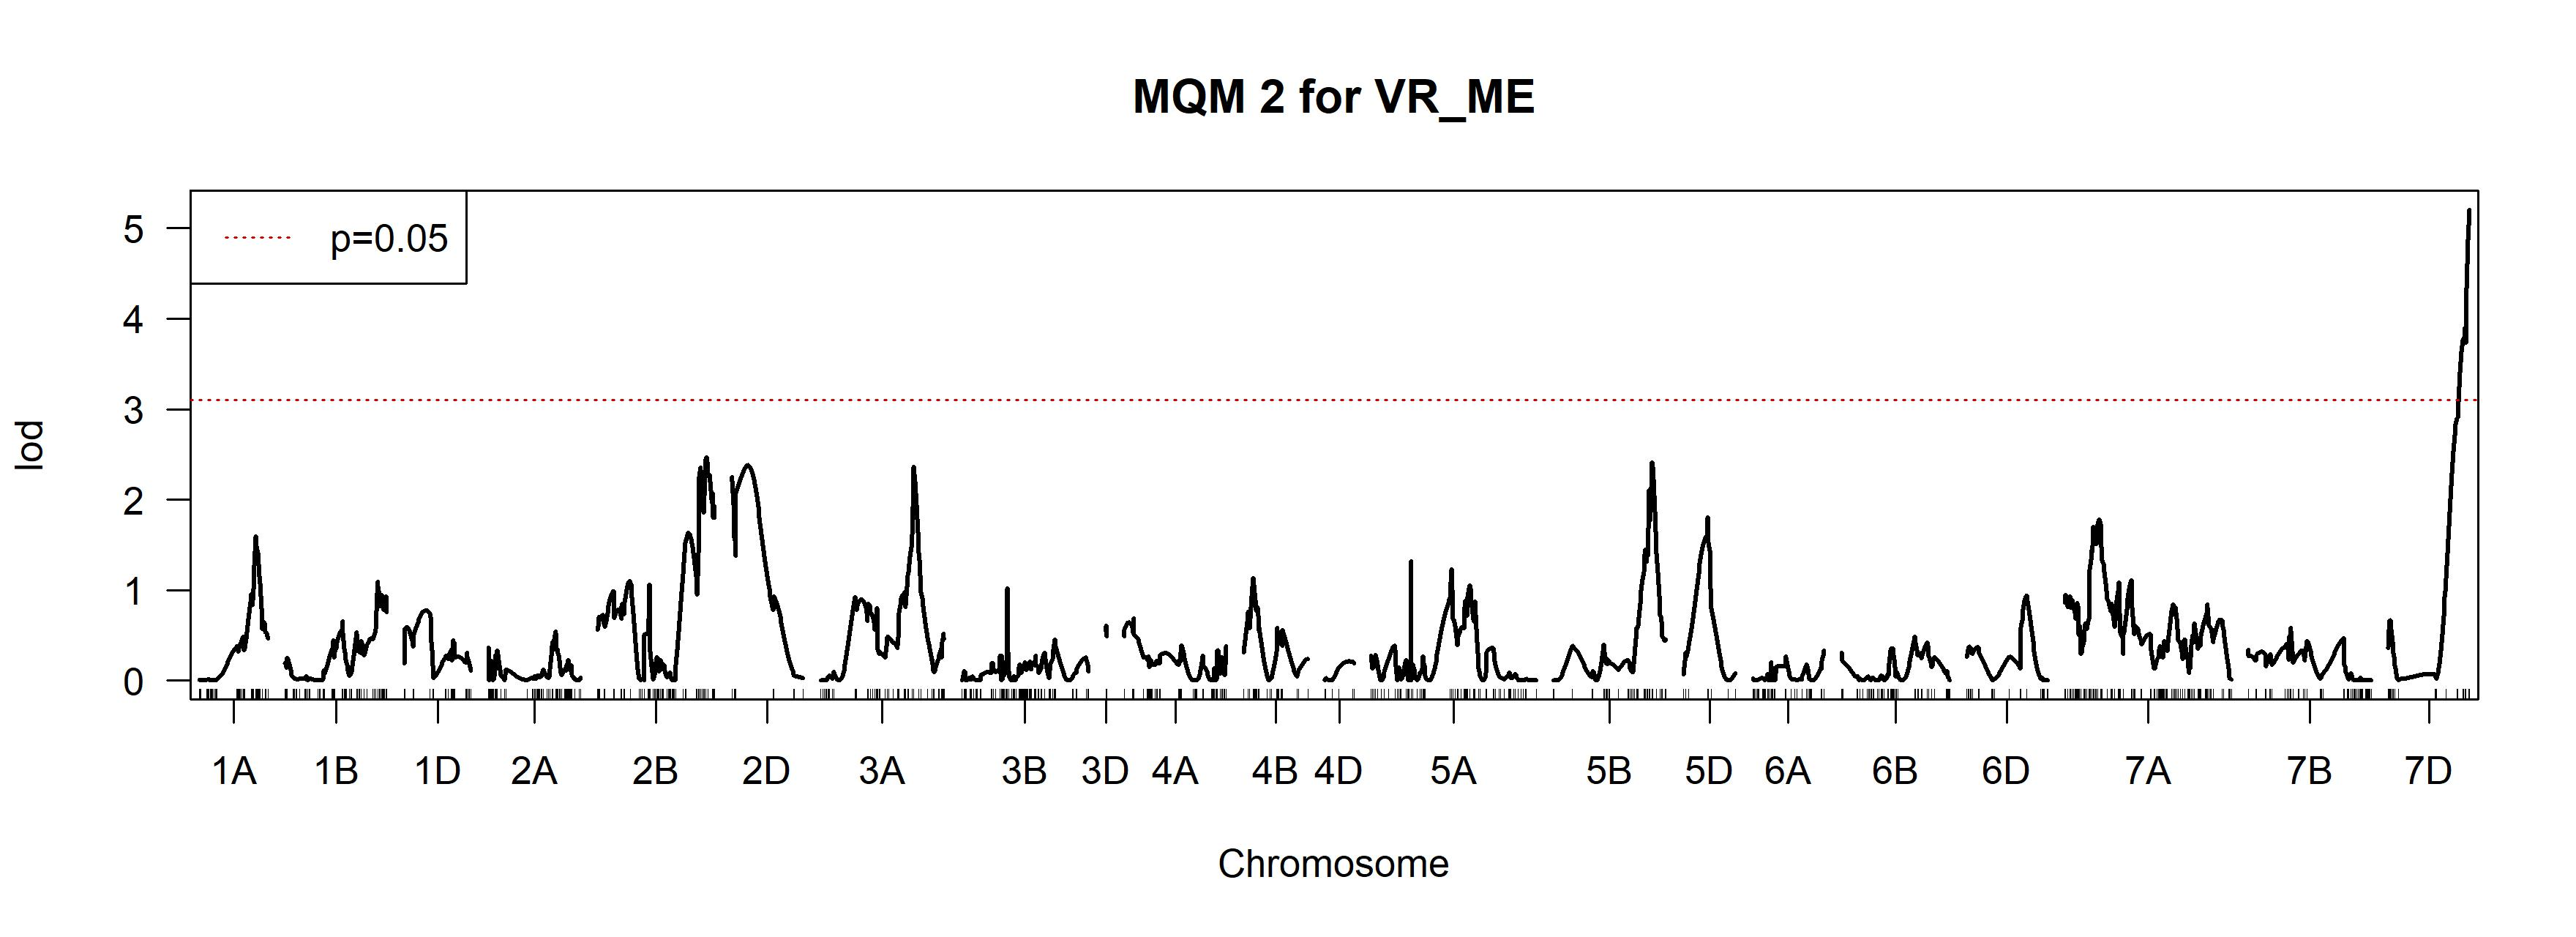
\includegraphics{Scan_MQM2_VR_ME.jpg}
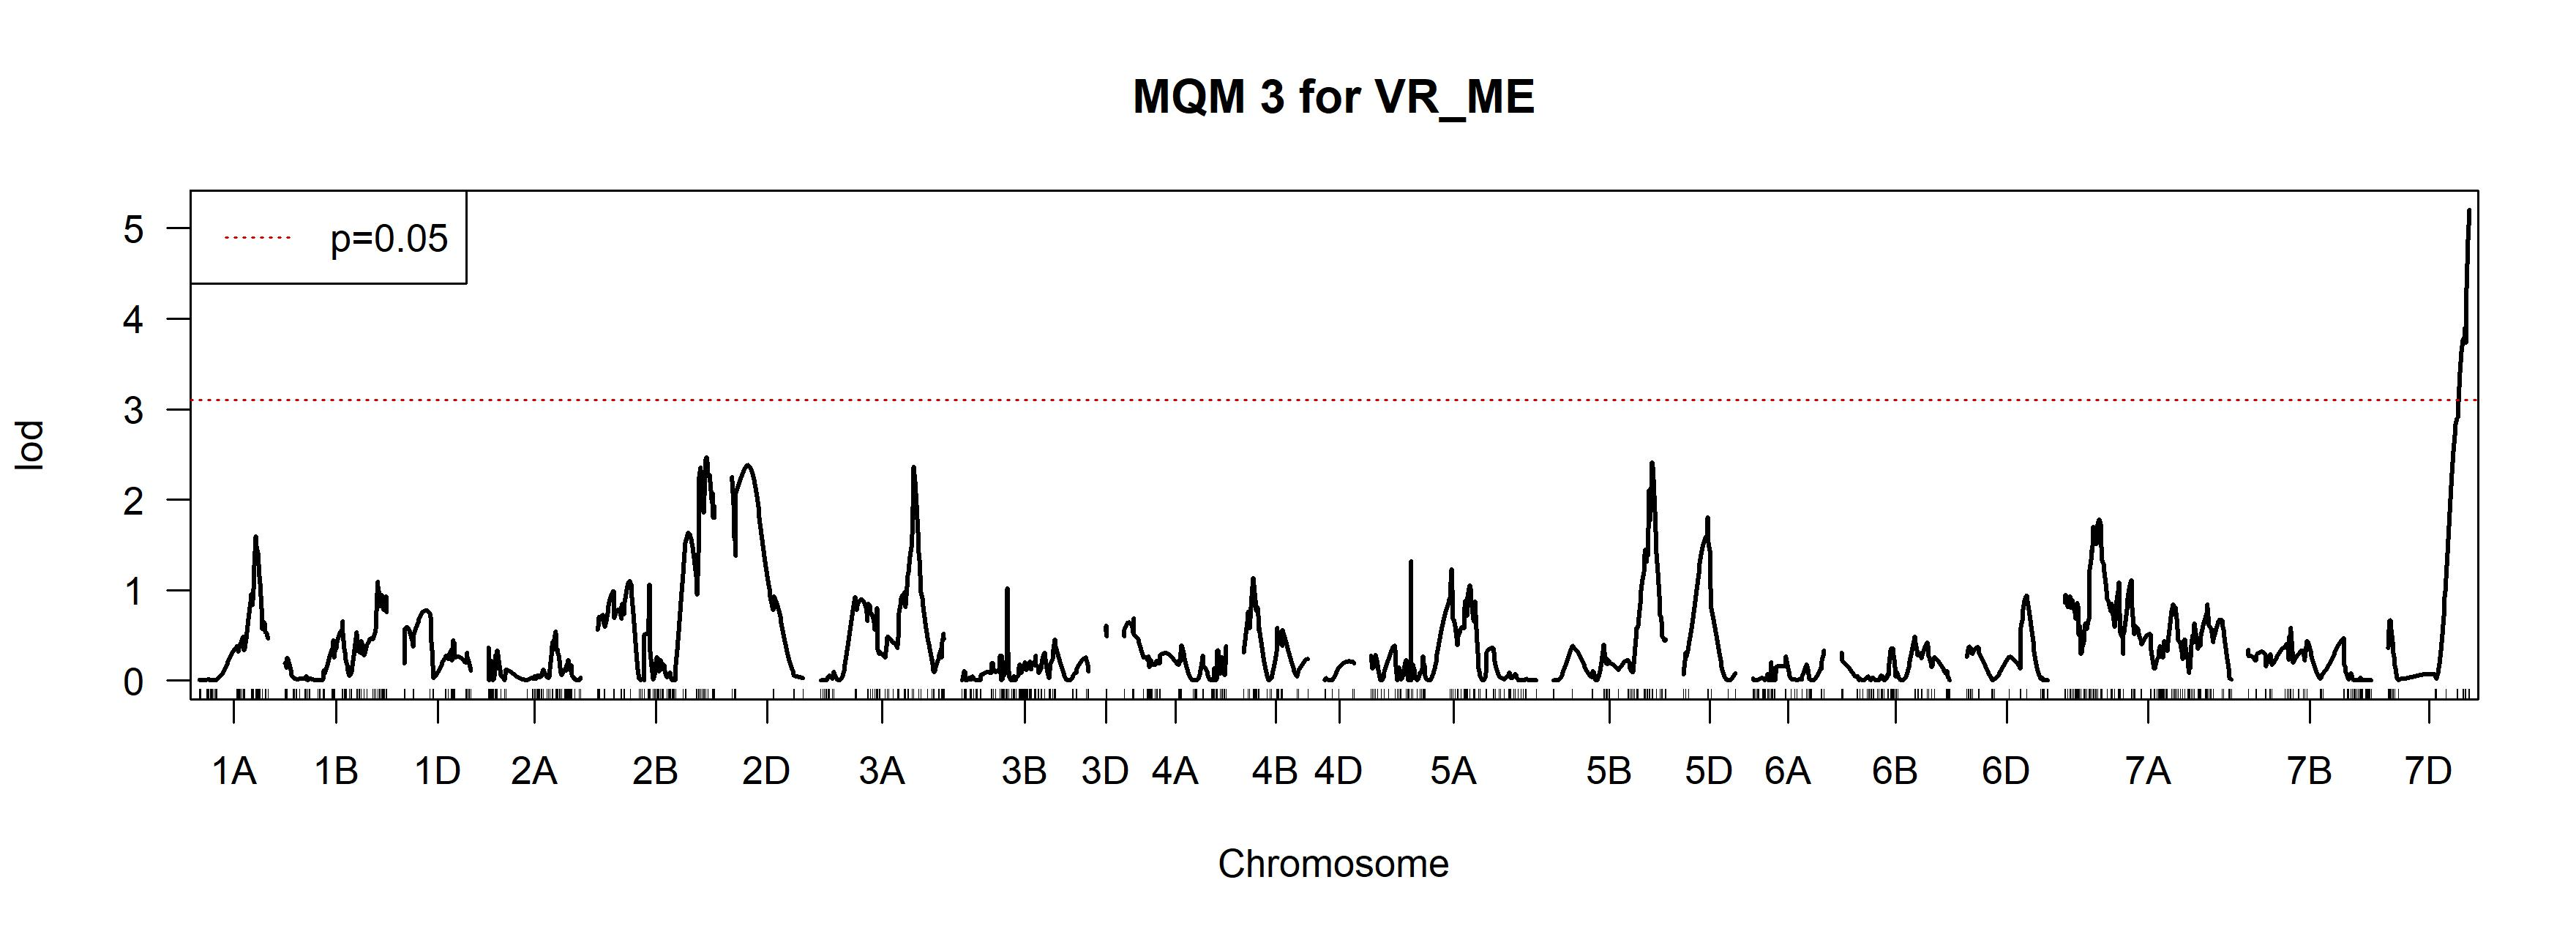
\includegraphics{Scan_MQM3_VR_ME.jpg}
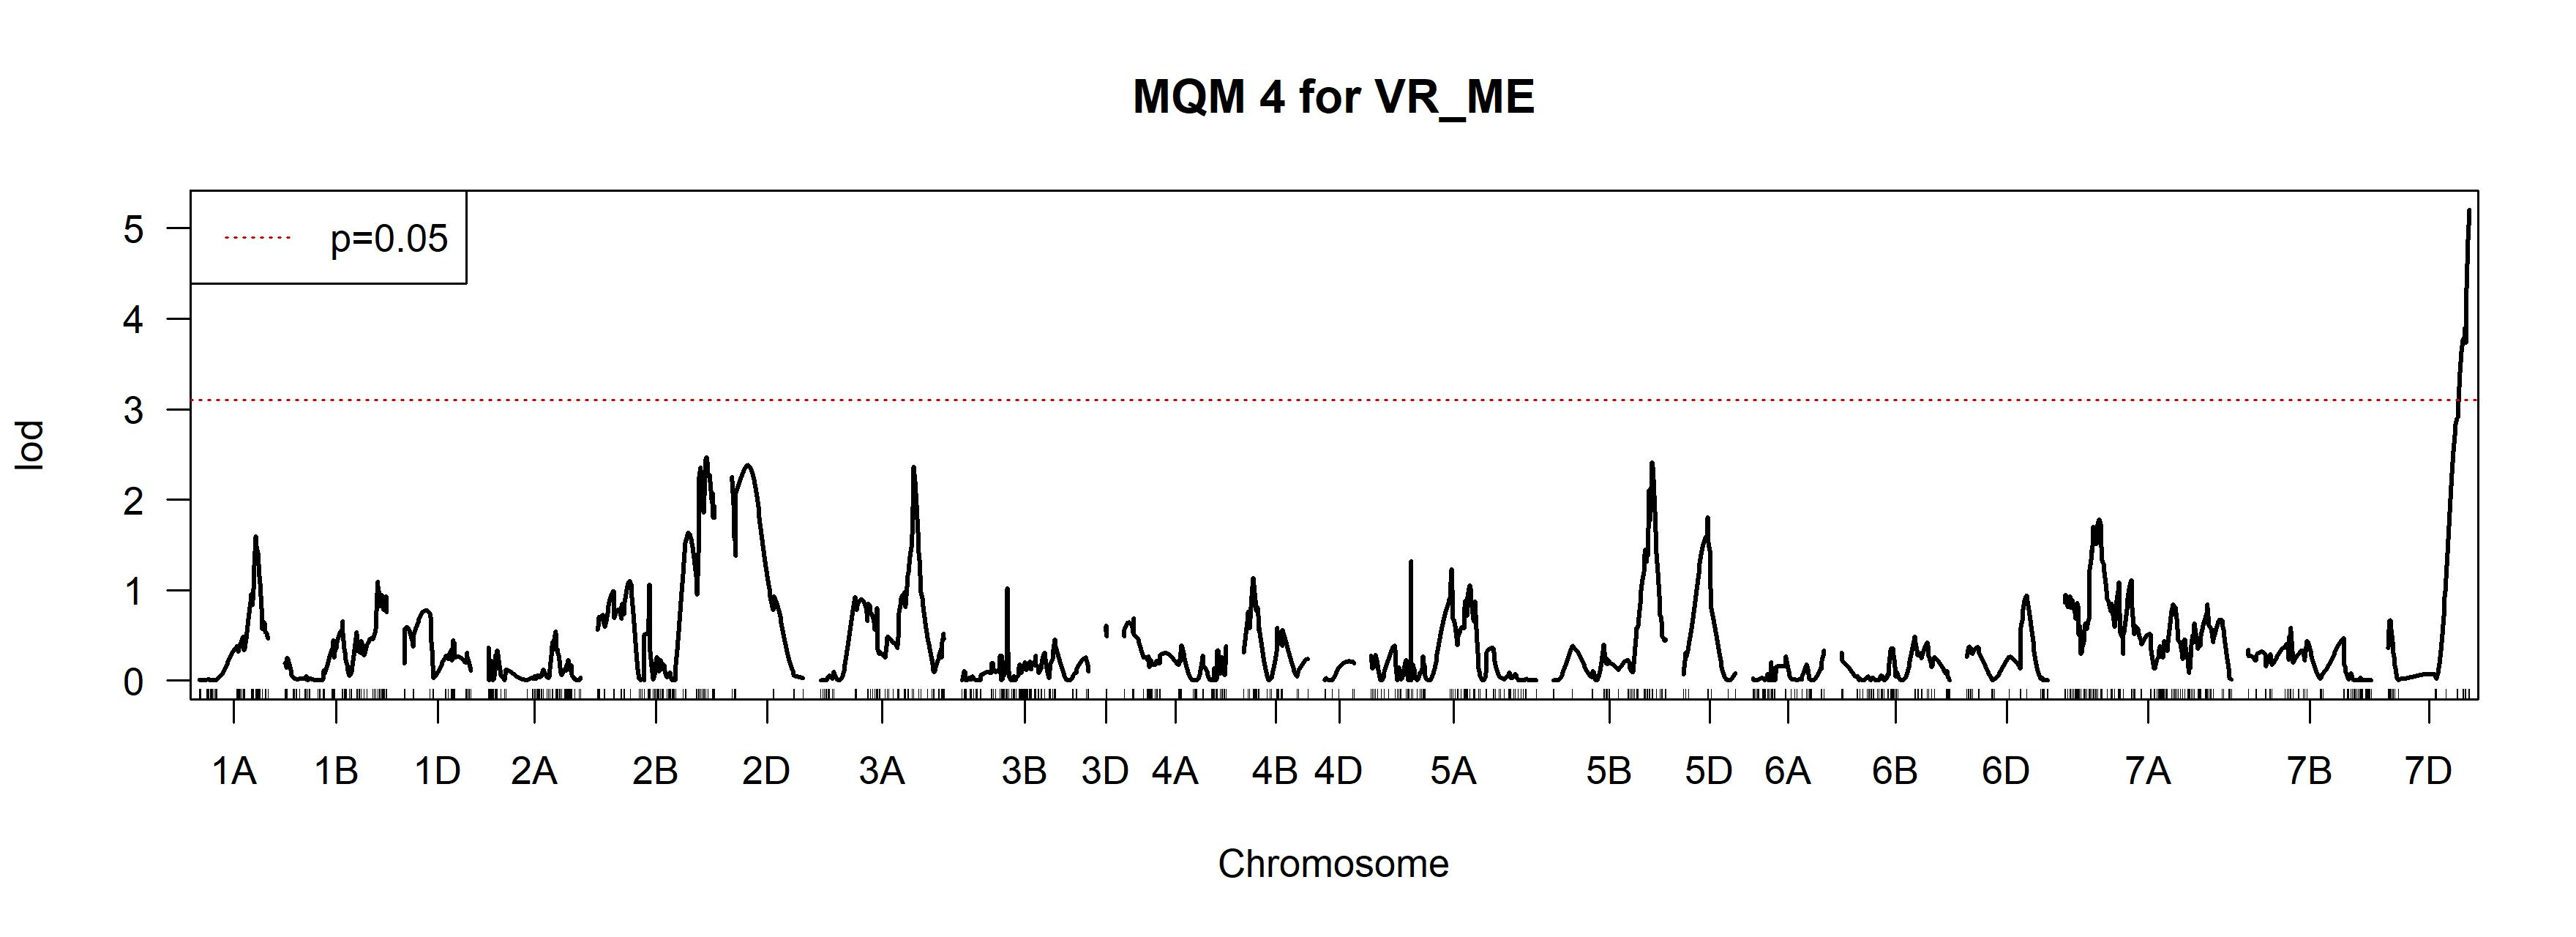
\includegraphics{Scan_MQM4_VR_ME.jpg}
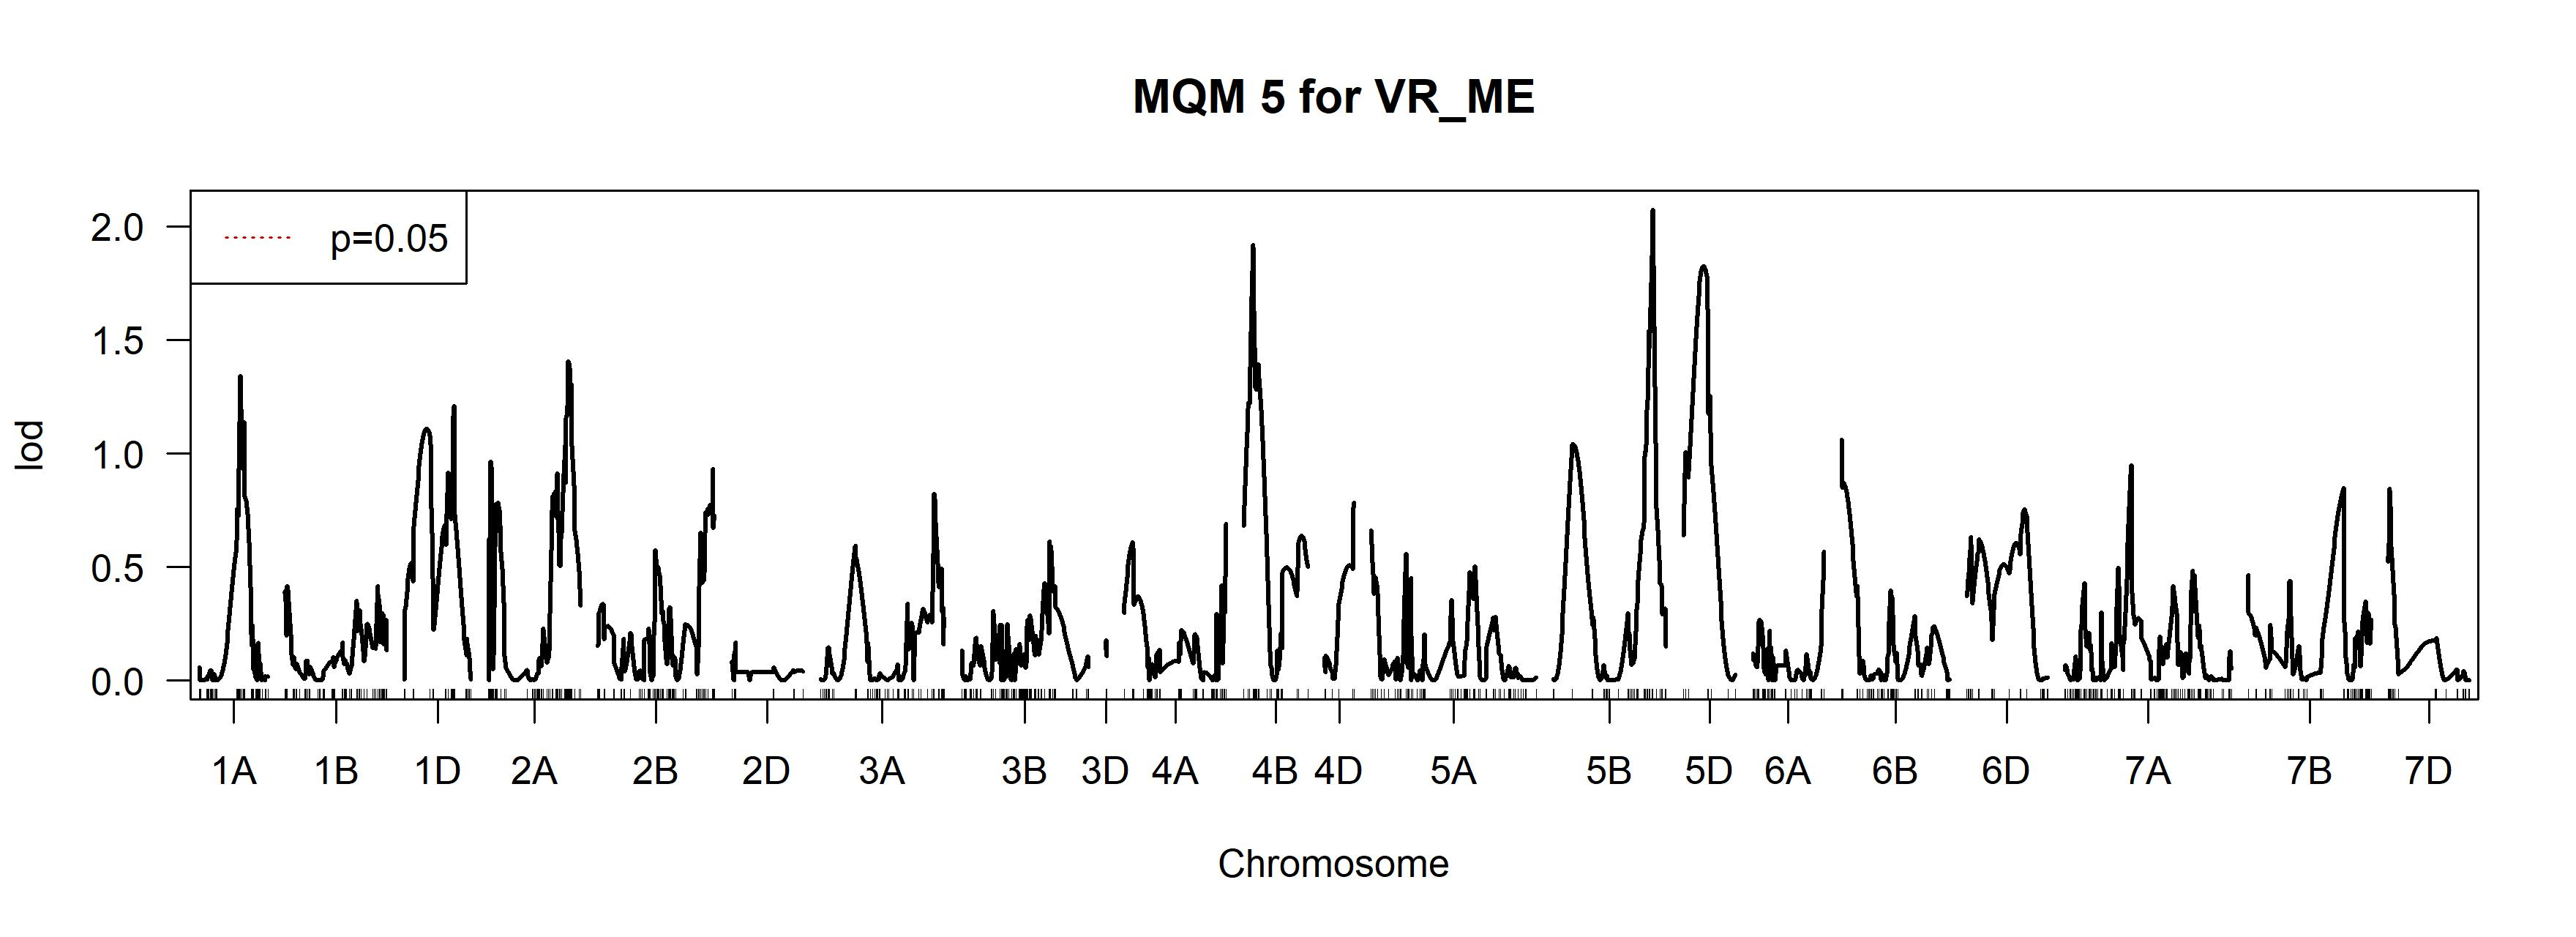
\includegraphics{Scan_MQM5_VR_ME.jpg} \pagebreak

\subsection{Visual Ratings in Kinston, NC -
2019}\label{visual-ratings-in-kinston-nc---2019}

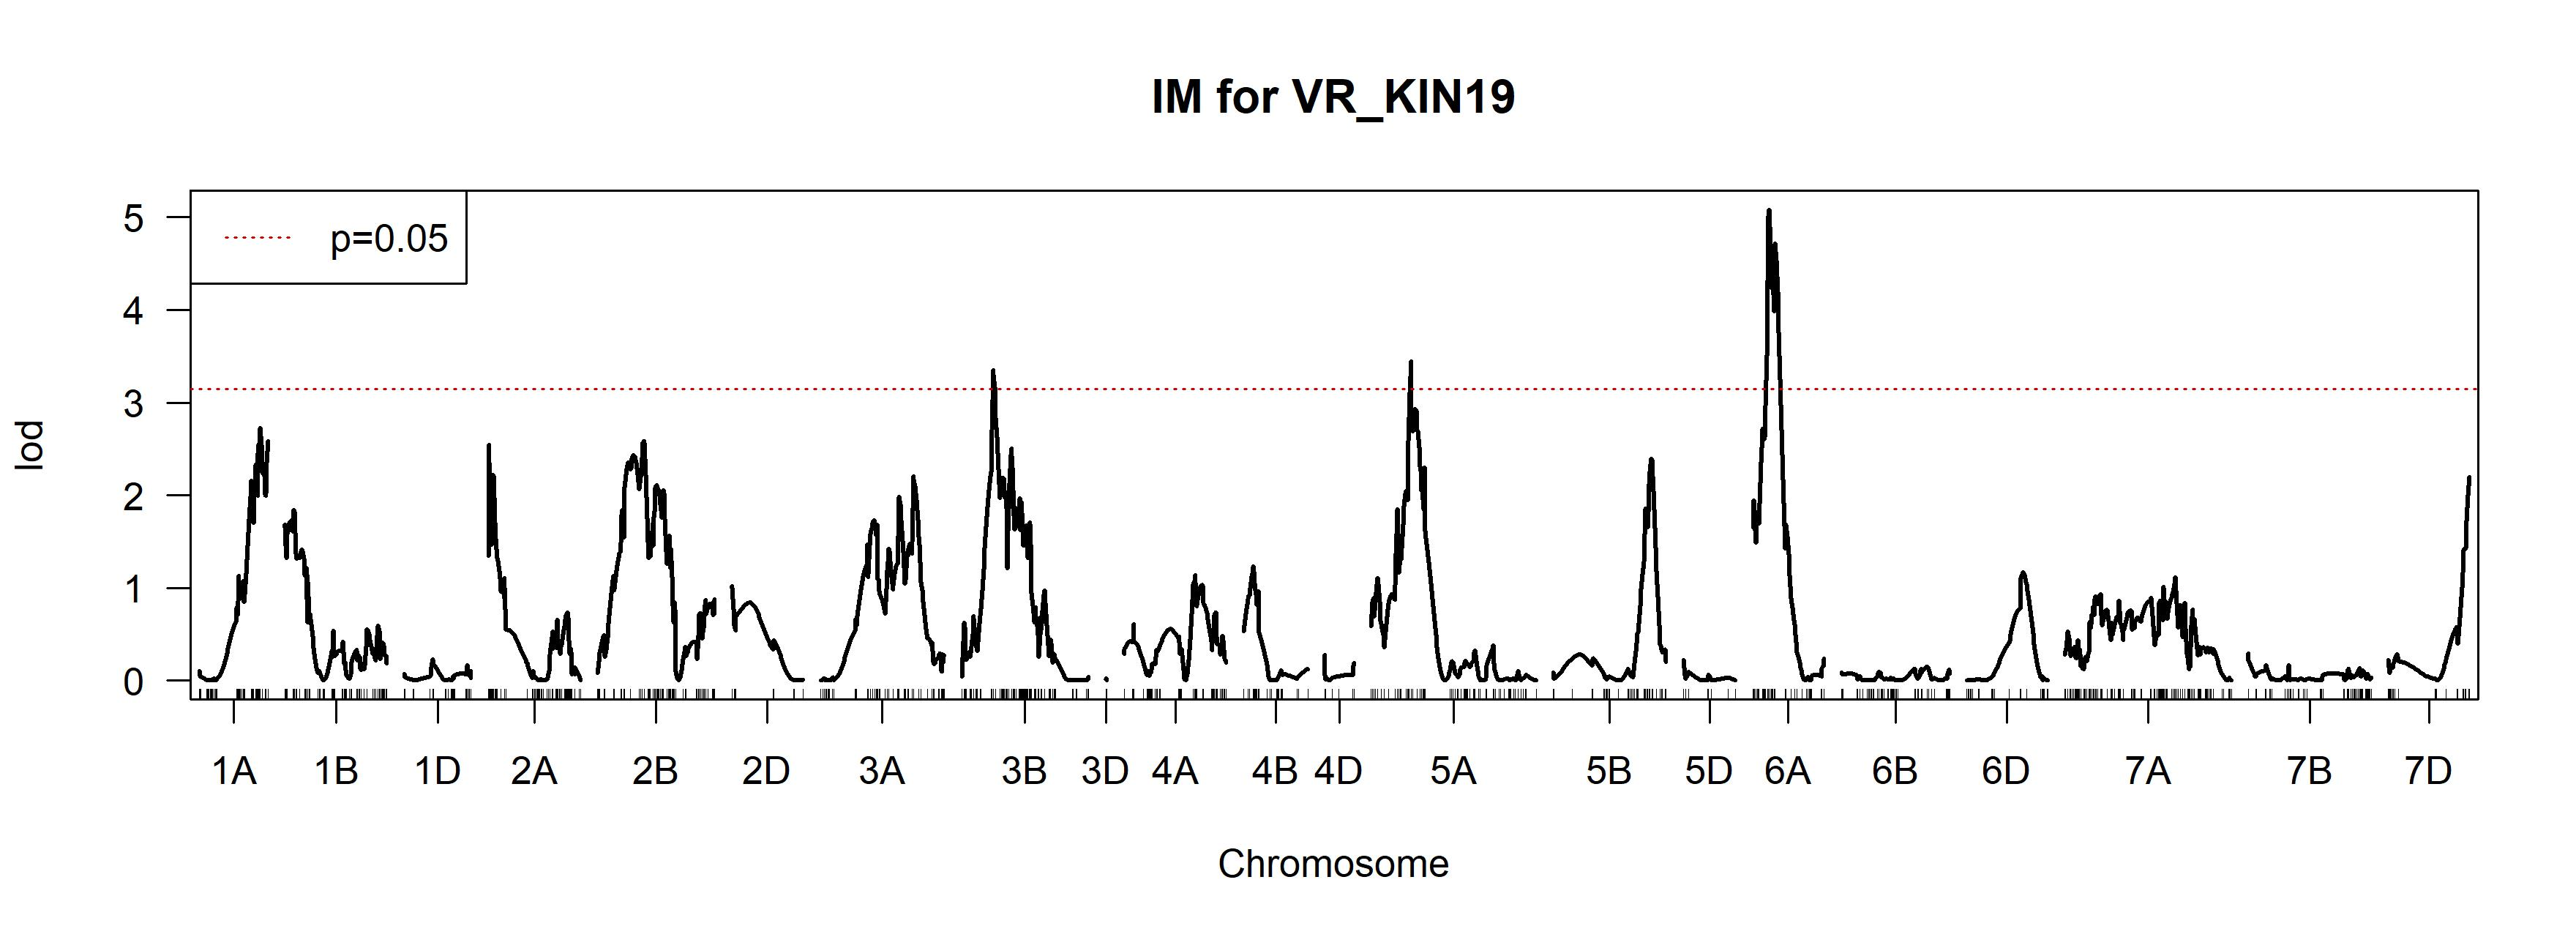
\includegraphics{Scan_IM_VR_KIN19.jpg}
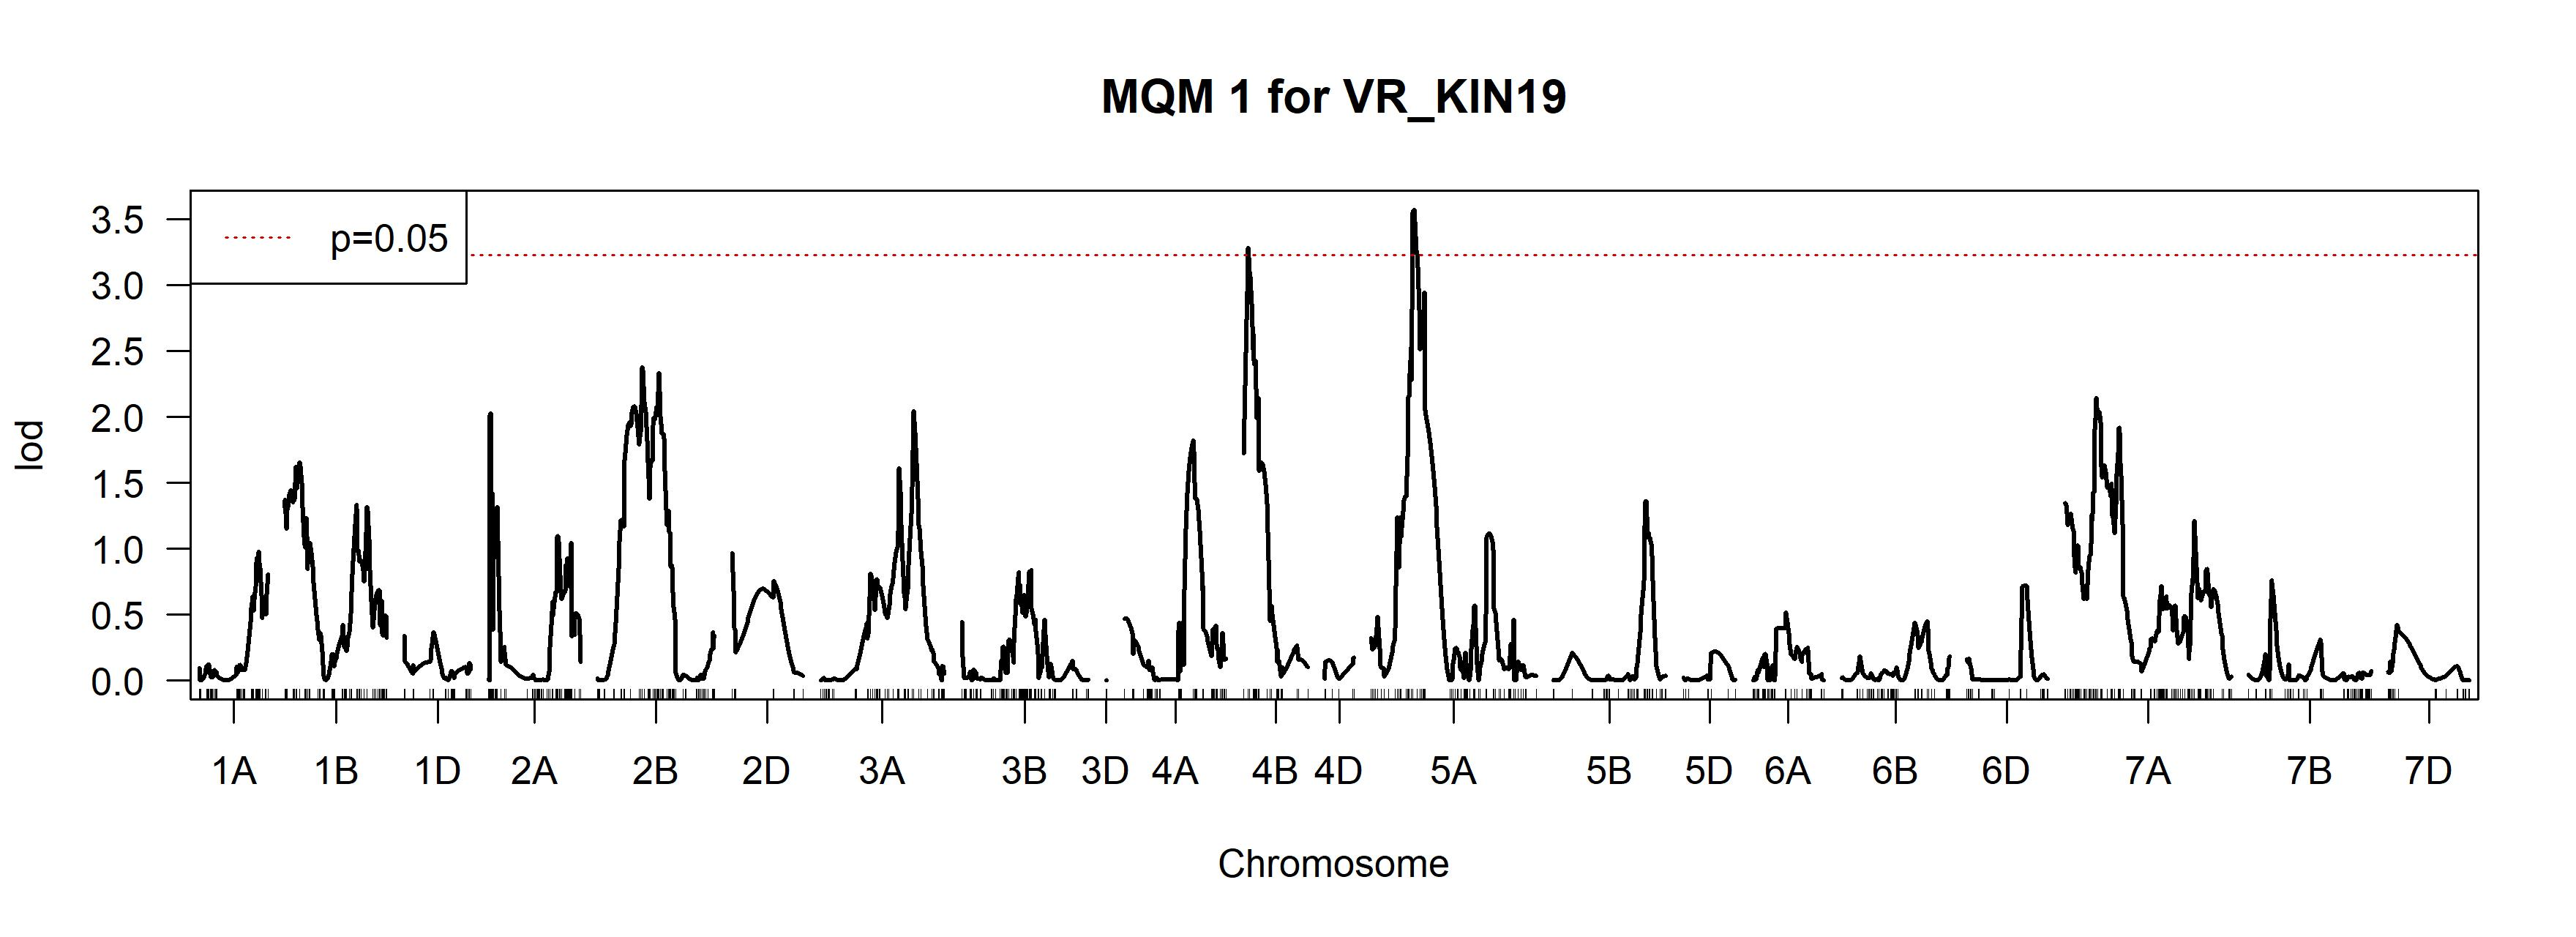
\includegraphics{Scan_MQM1_VR_KIN19.jpg}
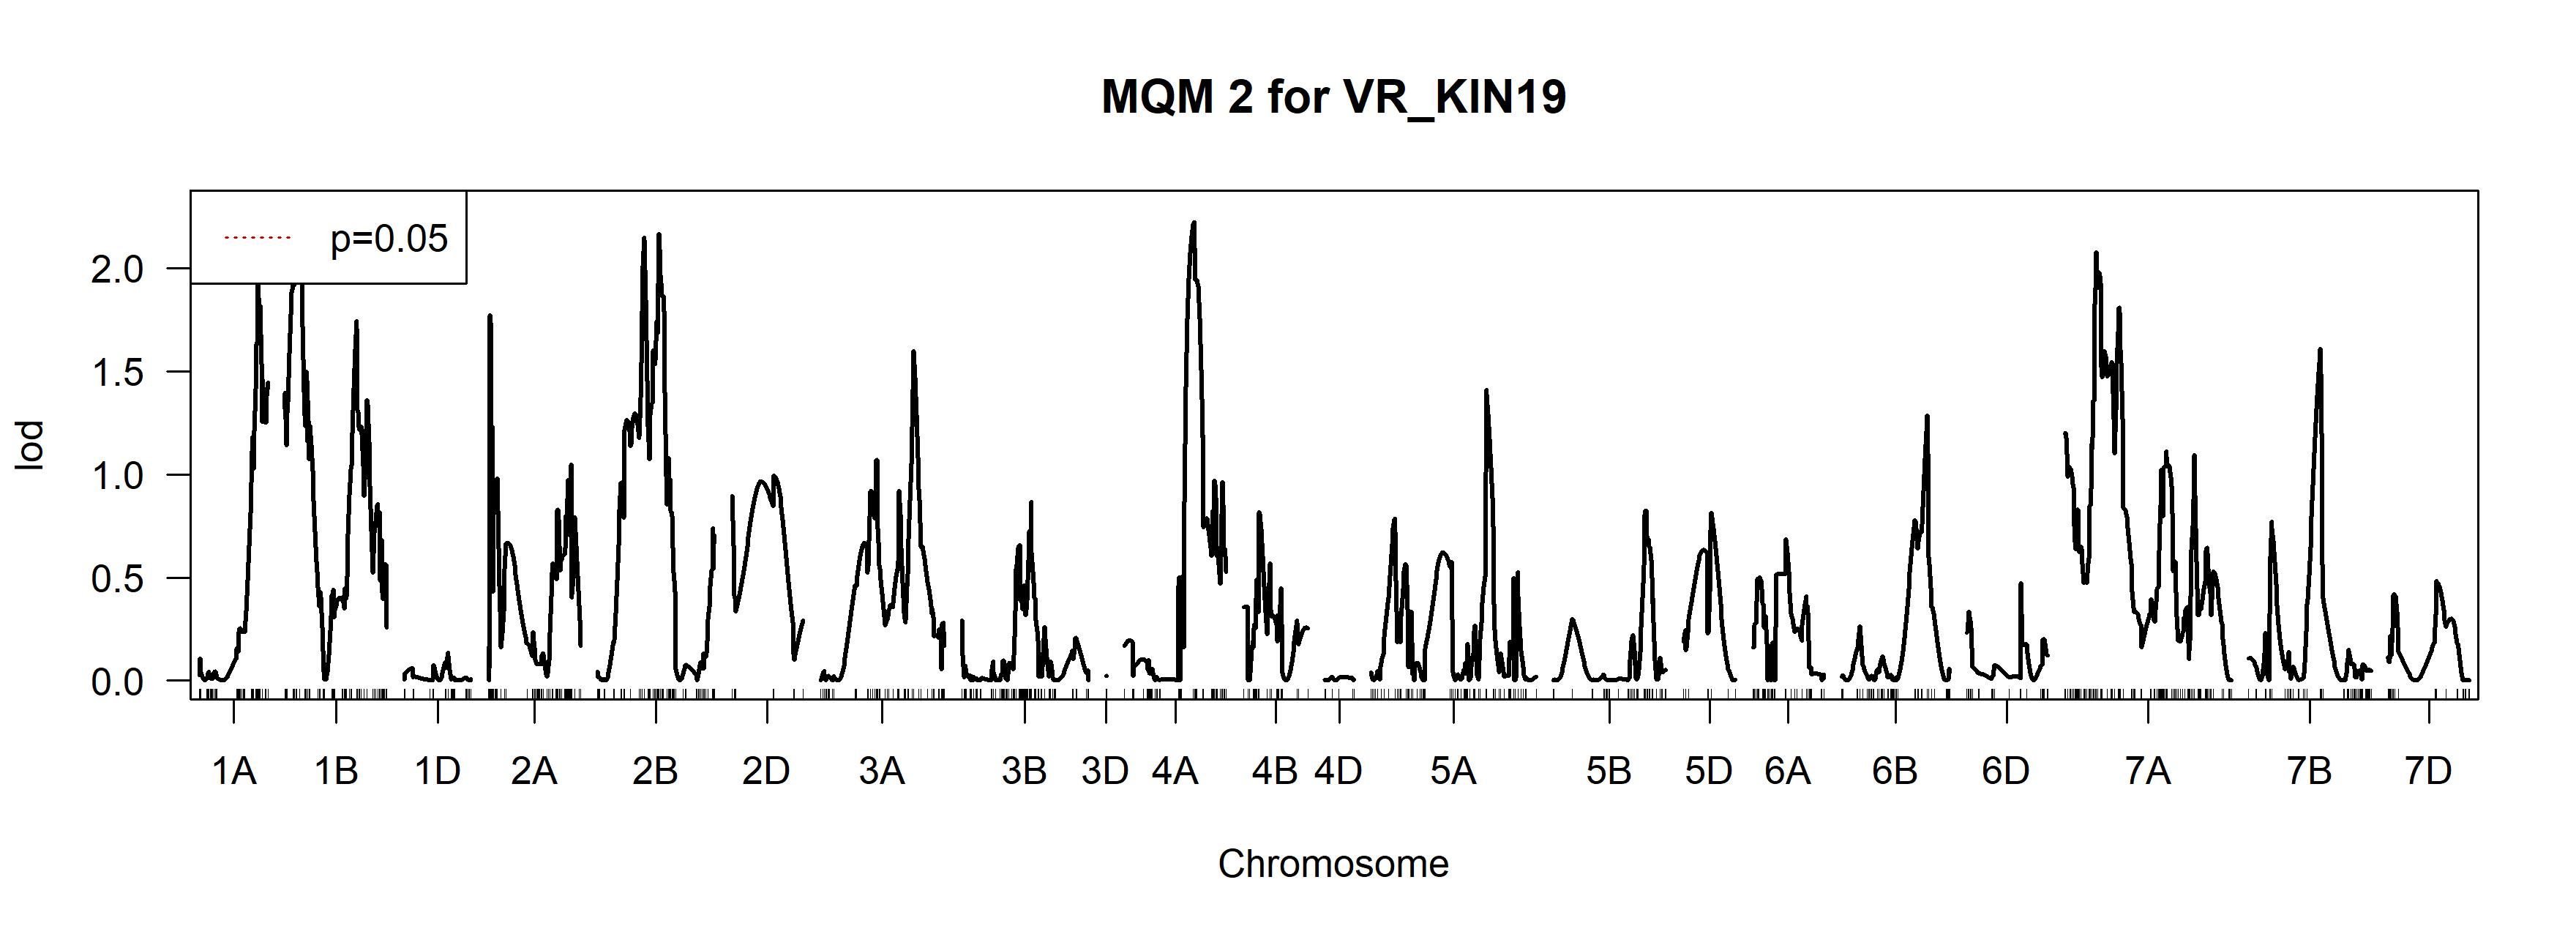
\includegraphics{Scan_MQM2_VR_KIN19.jpg} \pagebreak

\subsection{Visual Ratings in Kinston, NC -
2020}\label{visual-ratings-in-kinston-nc---2020}

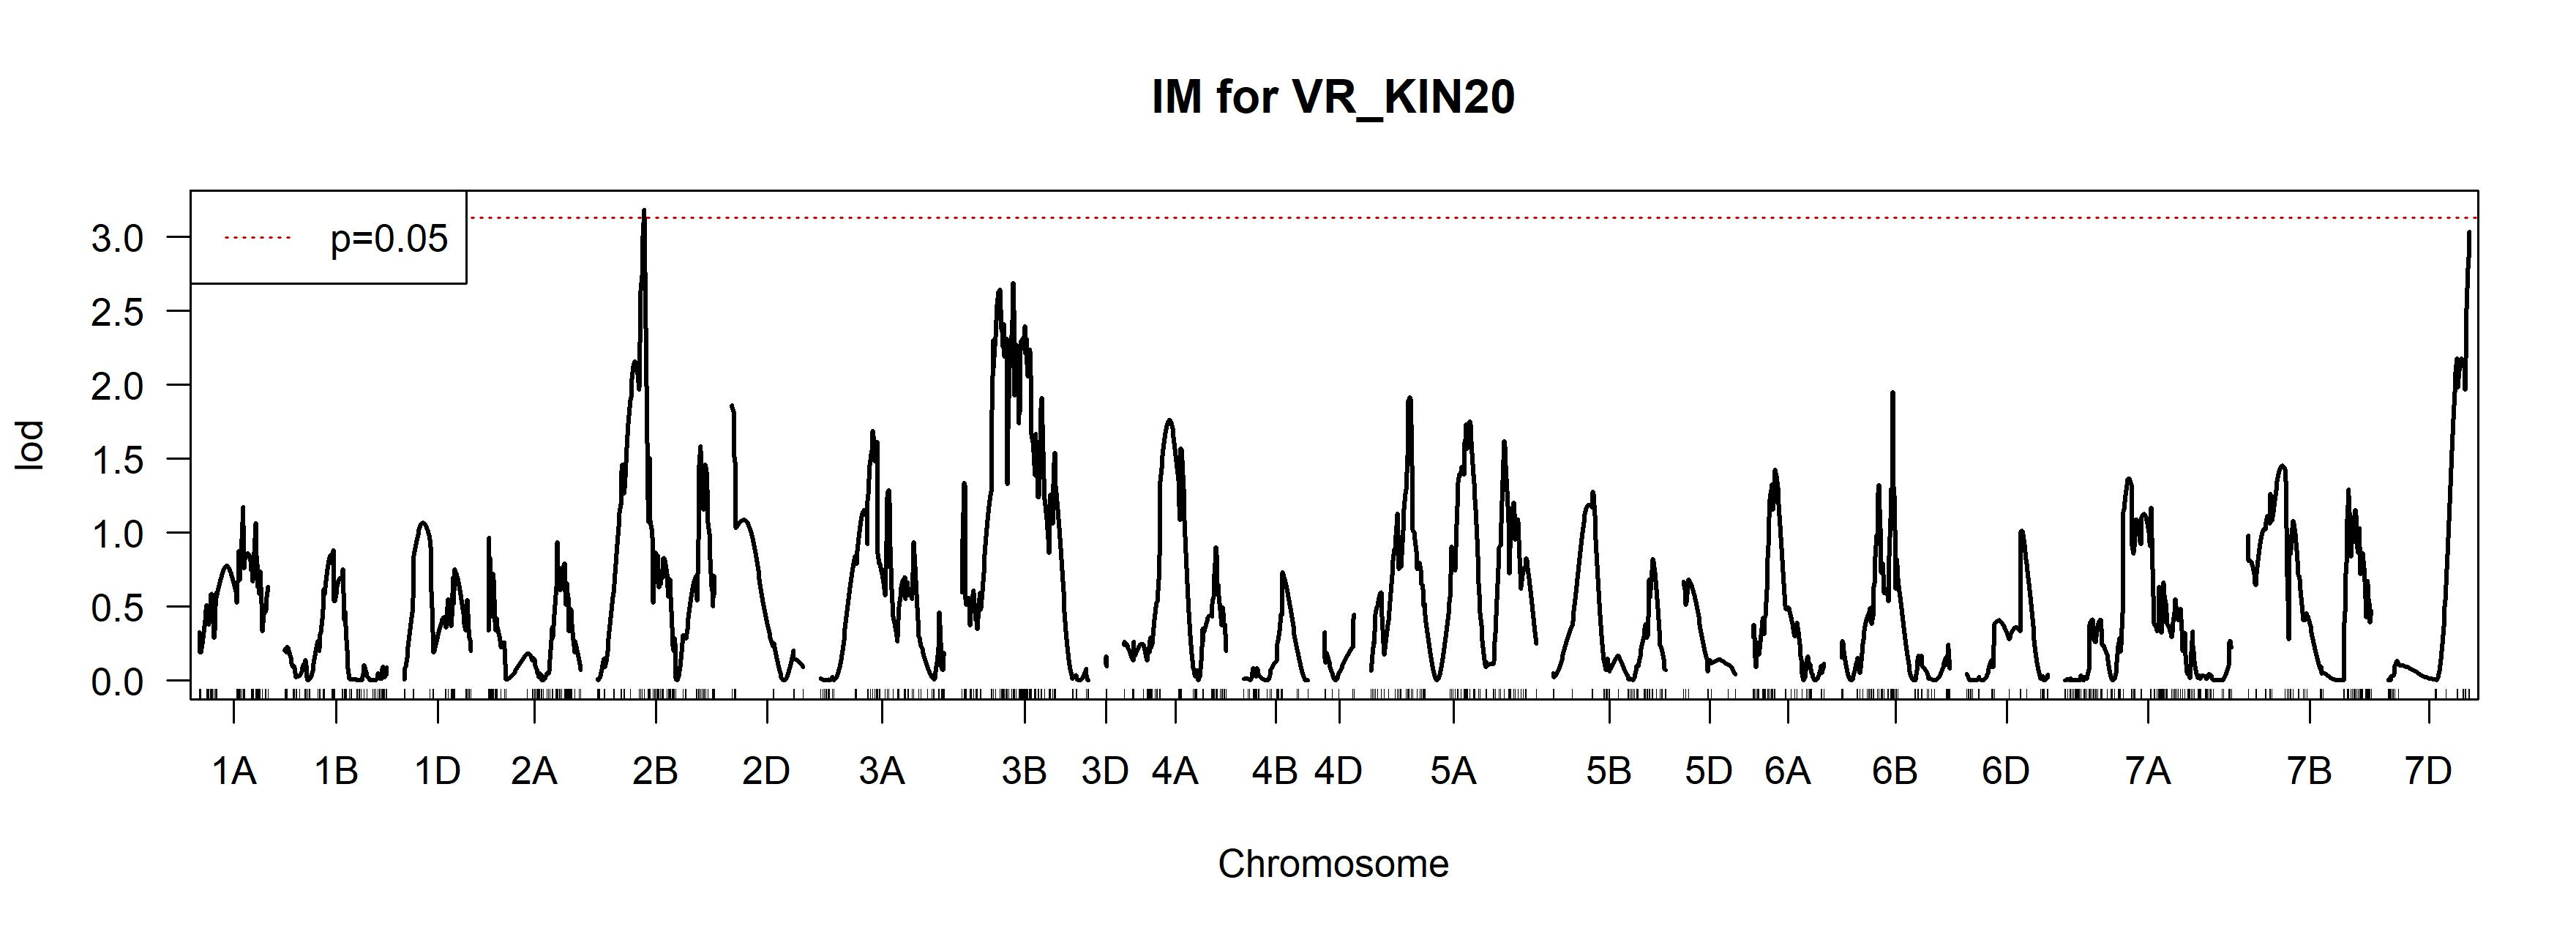
\includegraphics{Scan_IM_VR_KIN20.jpg}
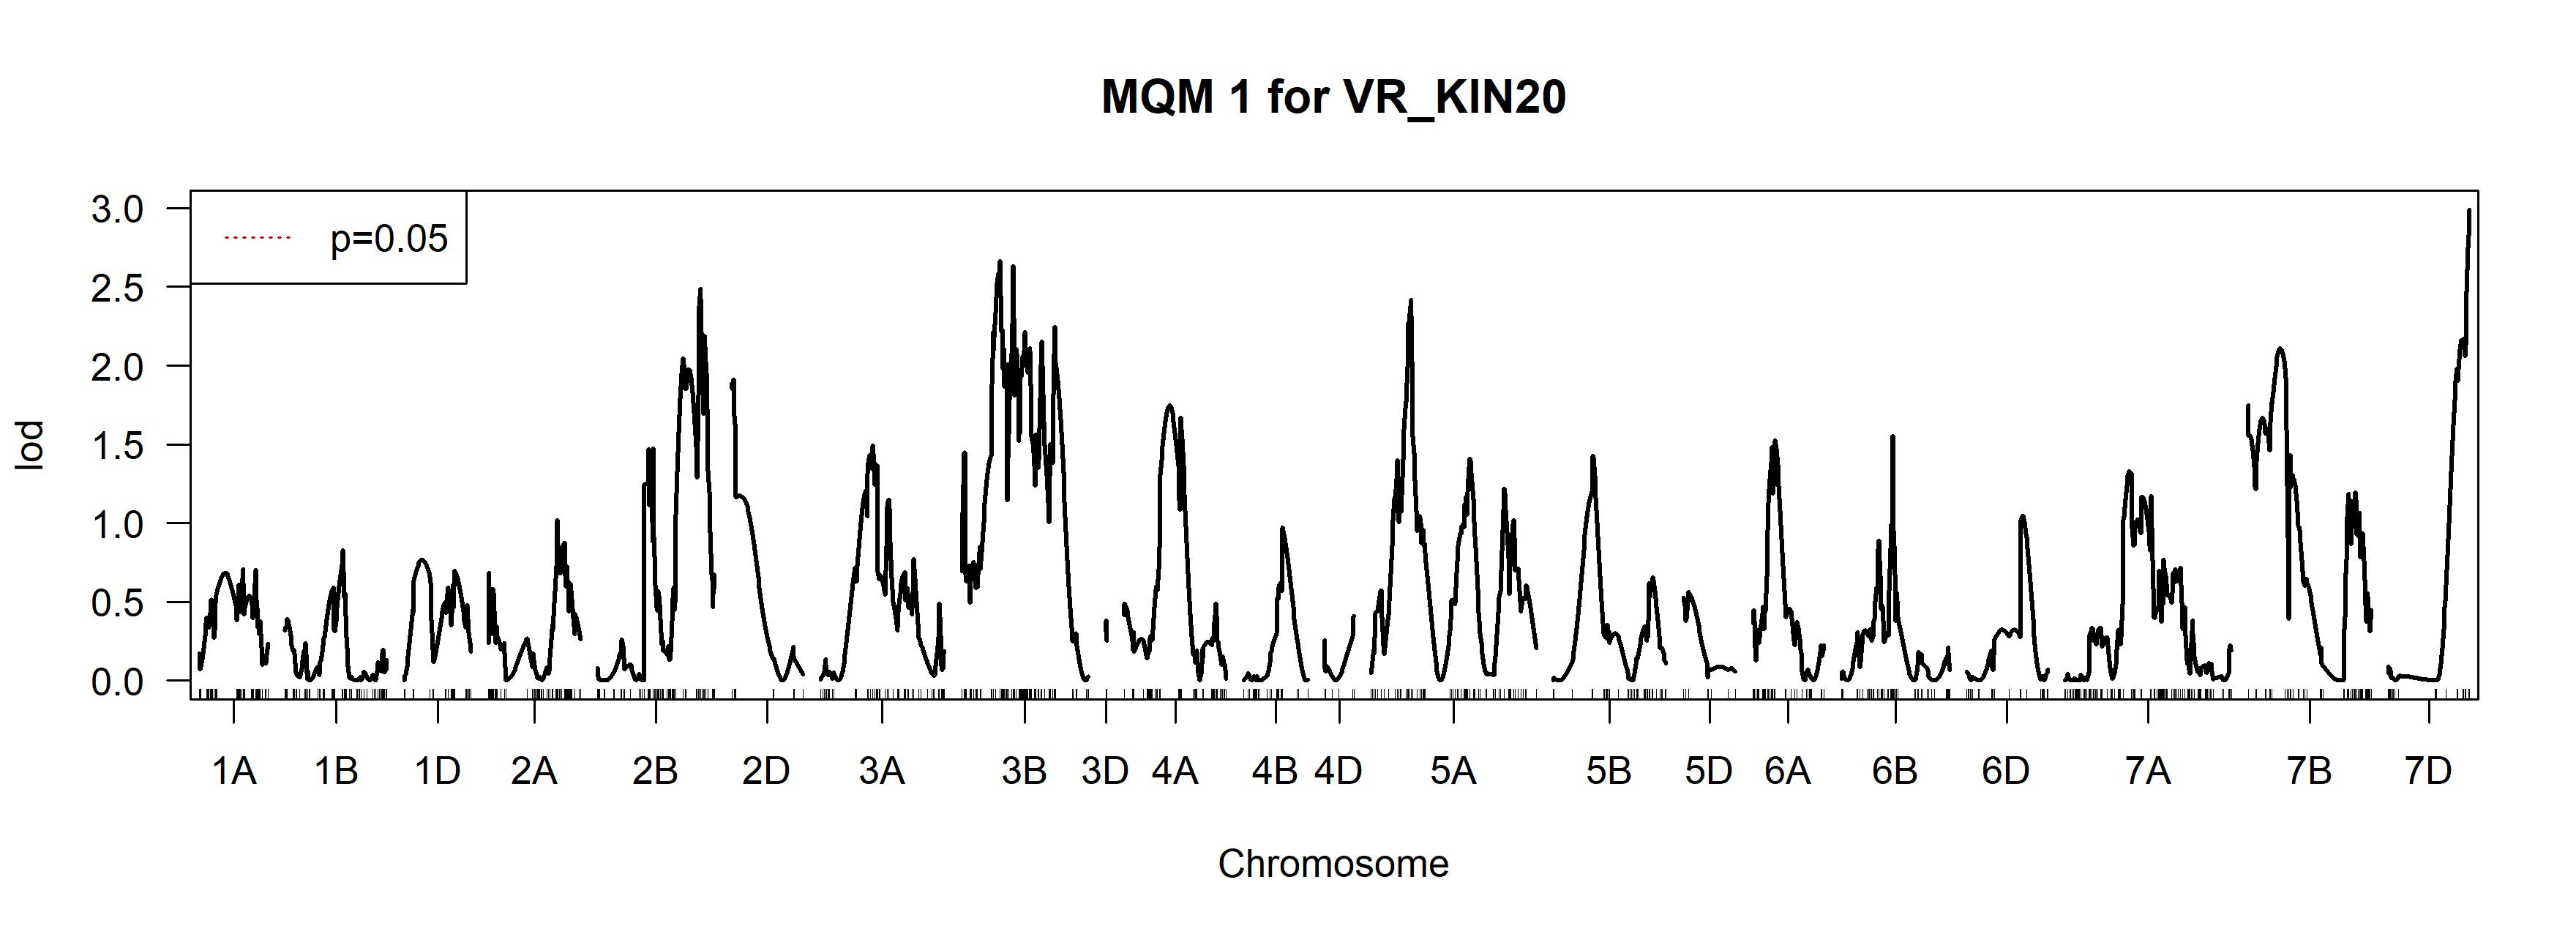
\includegraphics{Scan_MQM1_VR_KIN20.jpg} \pagebreak

\subsection{Visual Ratings in Raleigh, NC -
2019}\label{visual-ratings-in-raleigh-nc---2019}

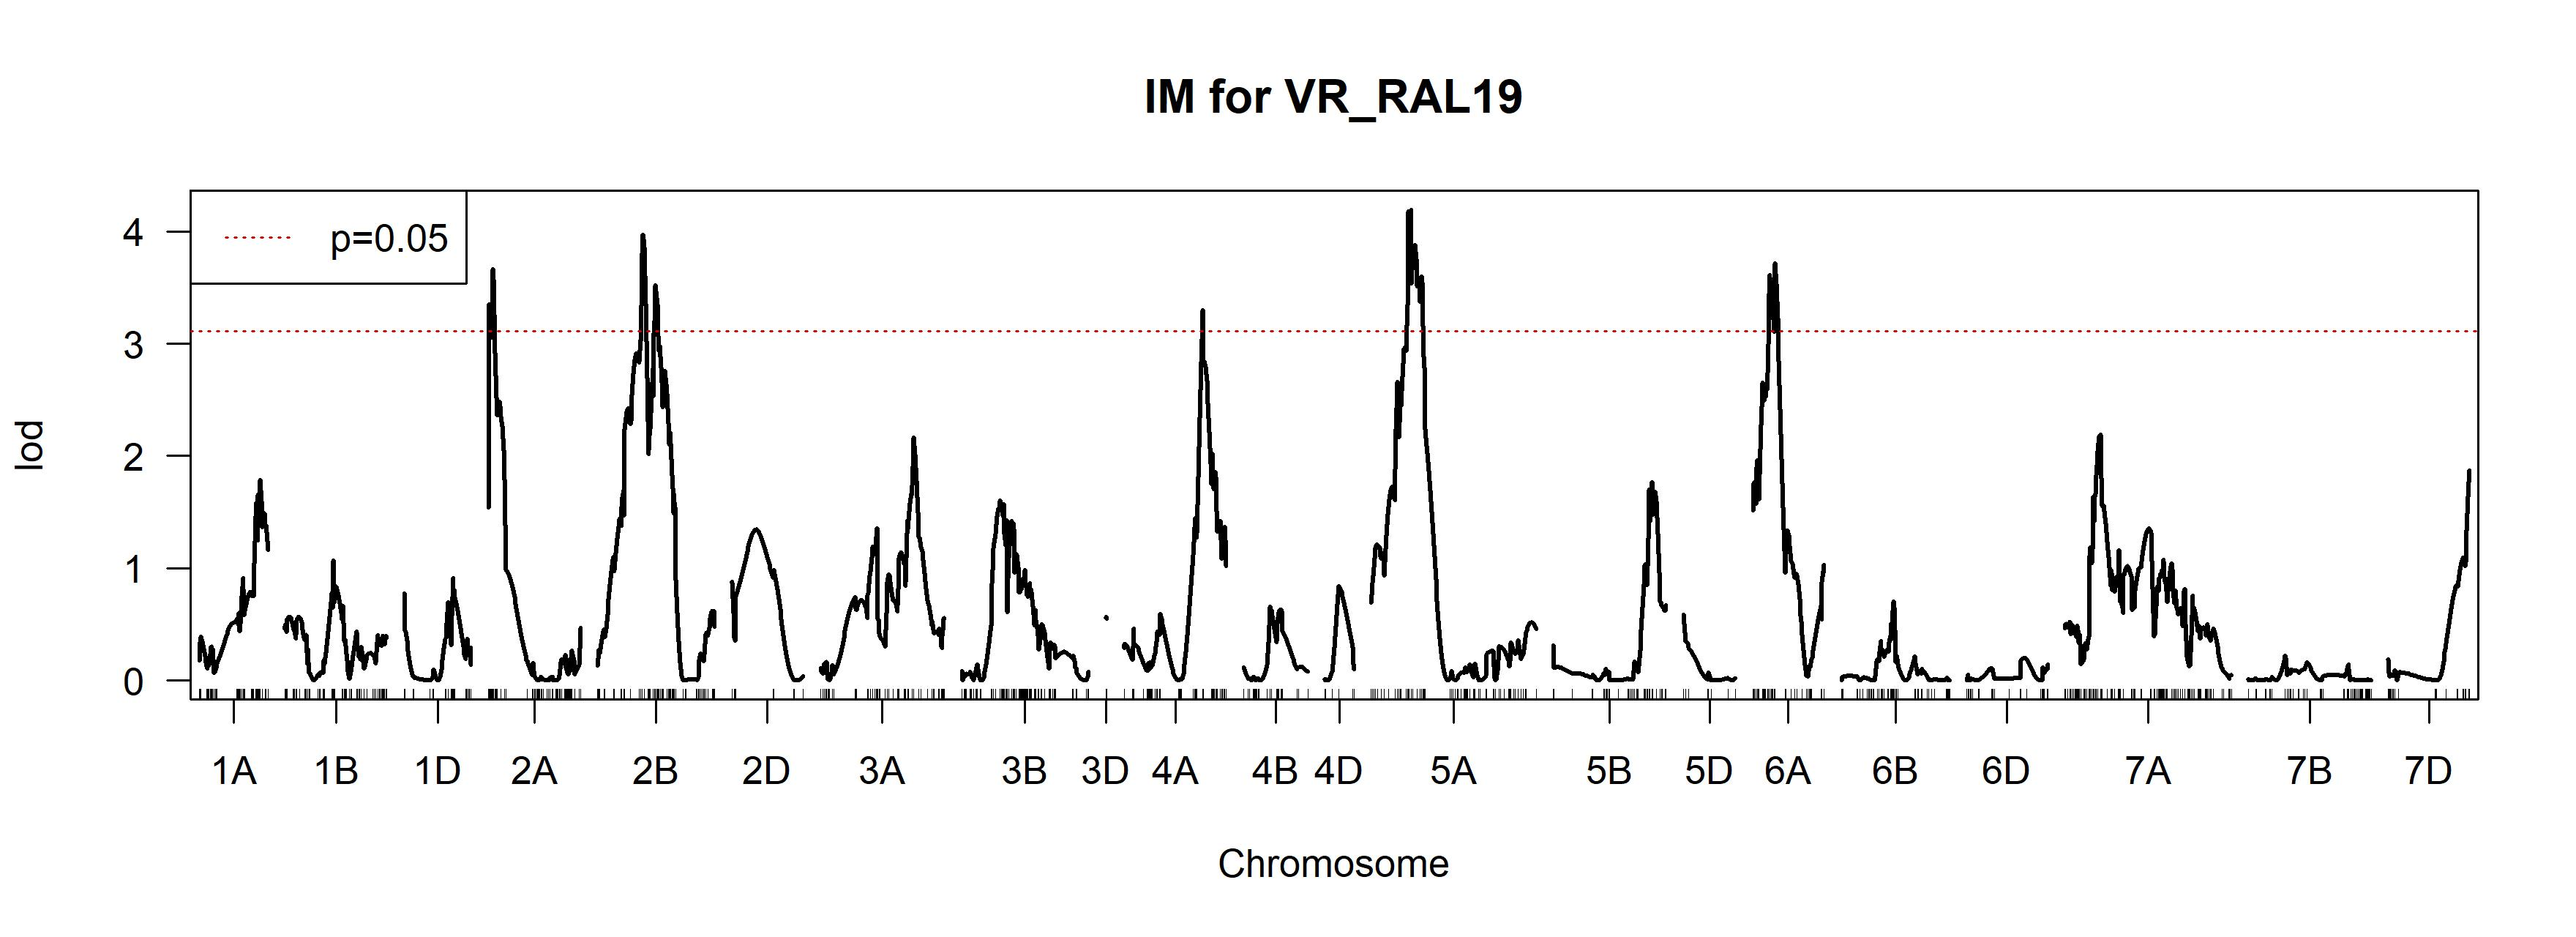
\includegraphics{Scan_IM_VR_RAL19.jpg}
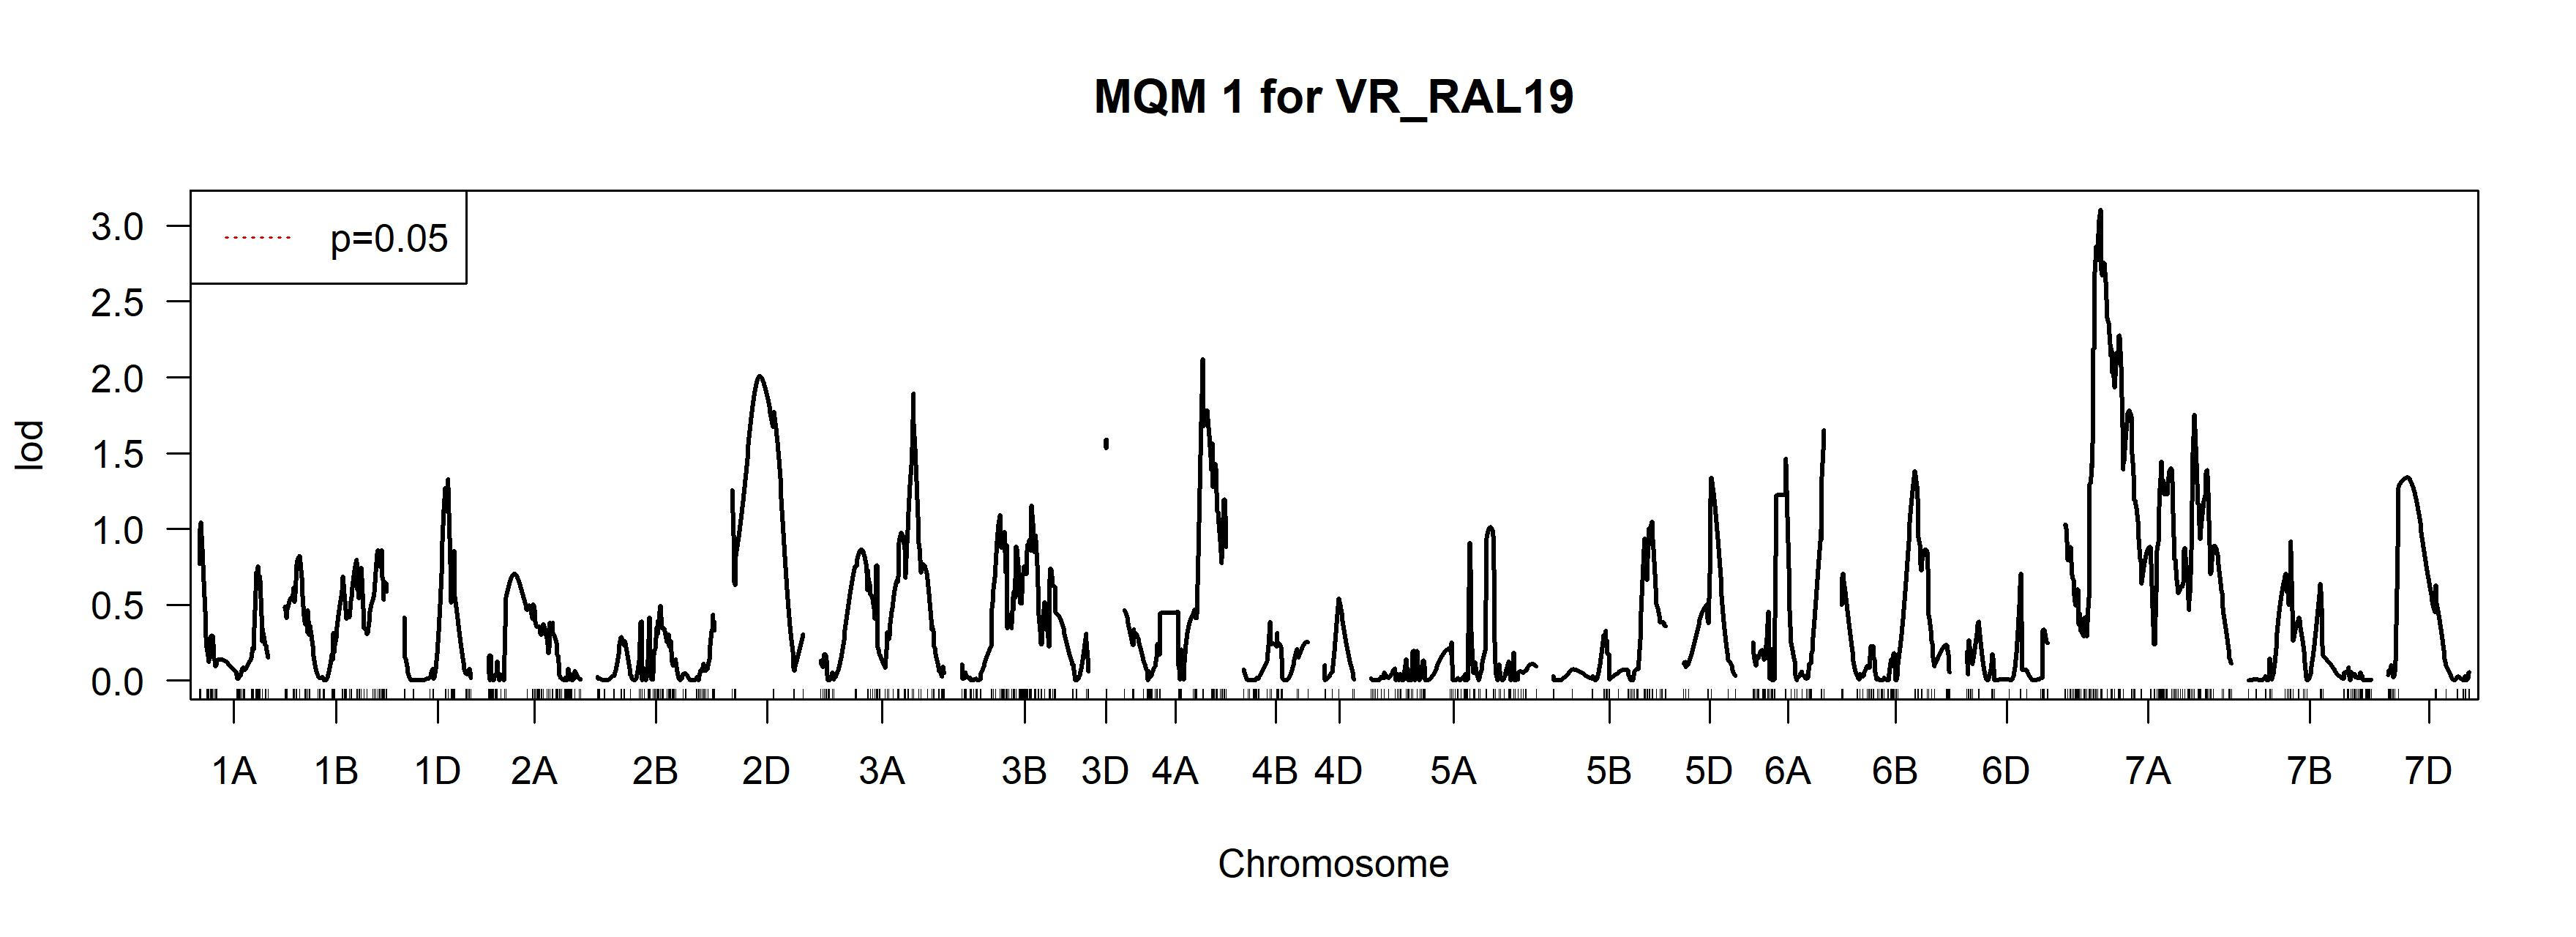
\includegraphics{Scan_MQM1_VR_RAL19.jpg} \pagebreak

\subsection{Visual Ratings in Raleigh, NC -
2020}\label{visual-ratings-in-raleigh-nc---2020}

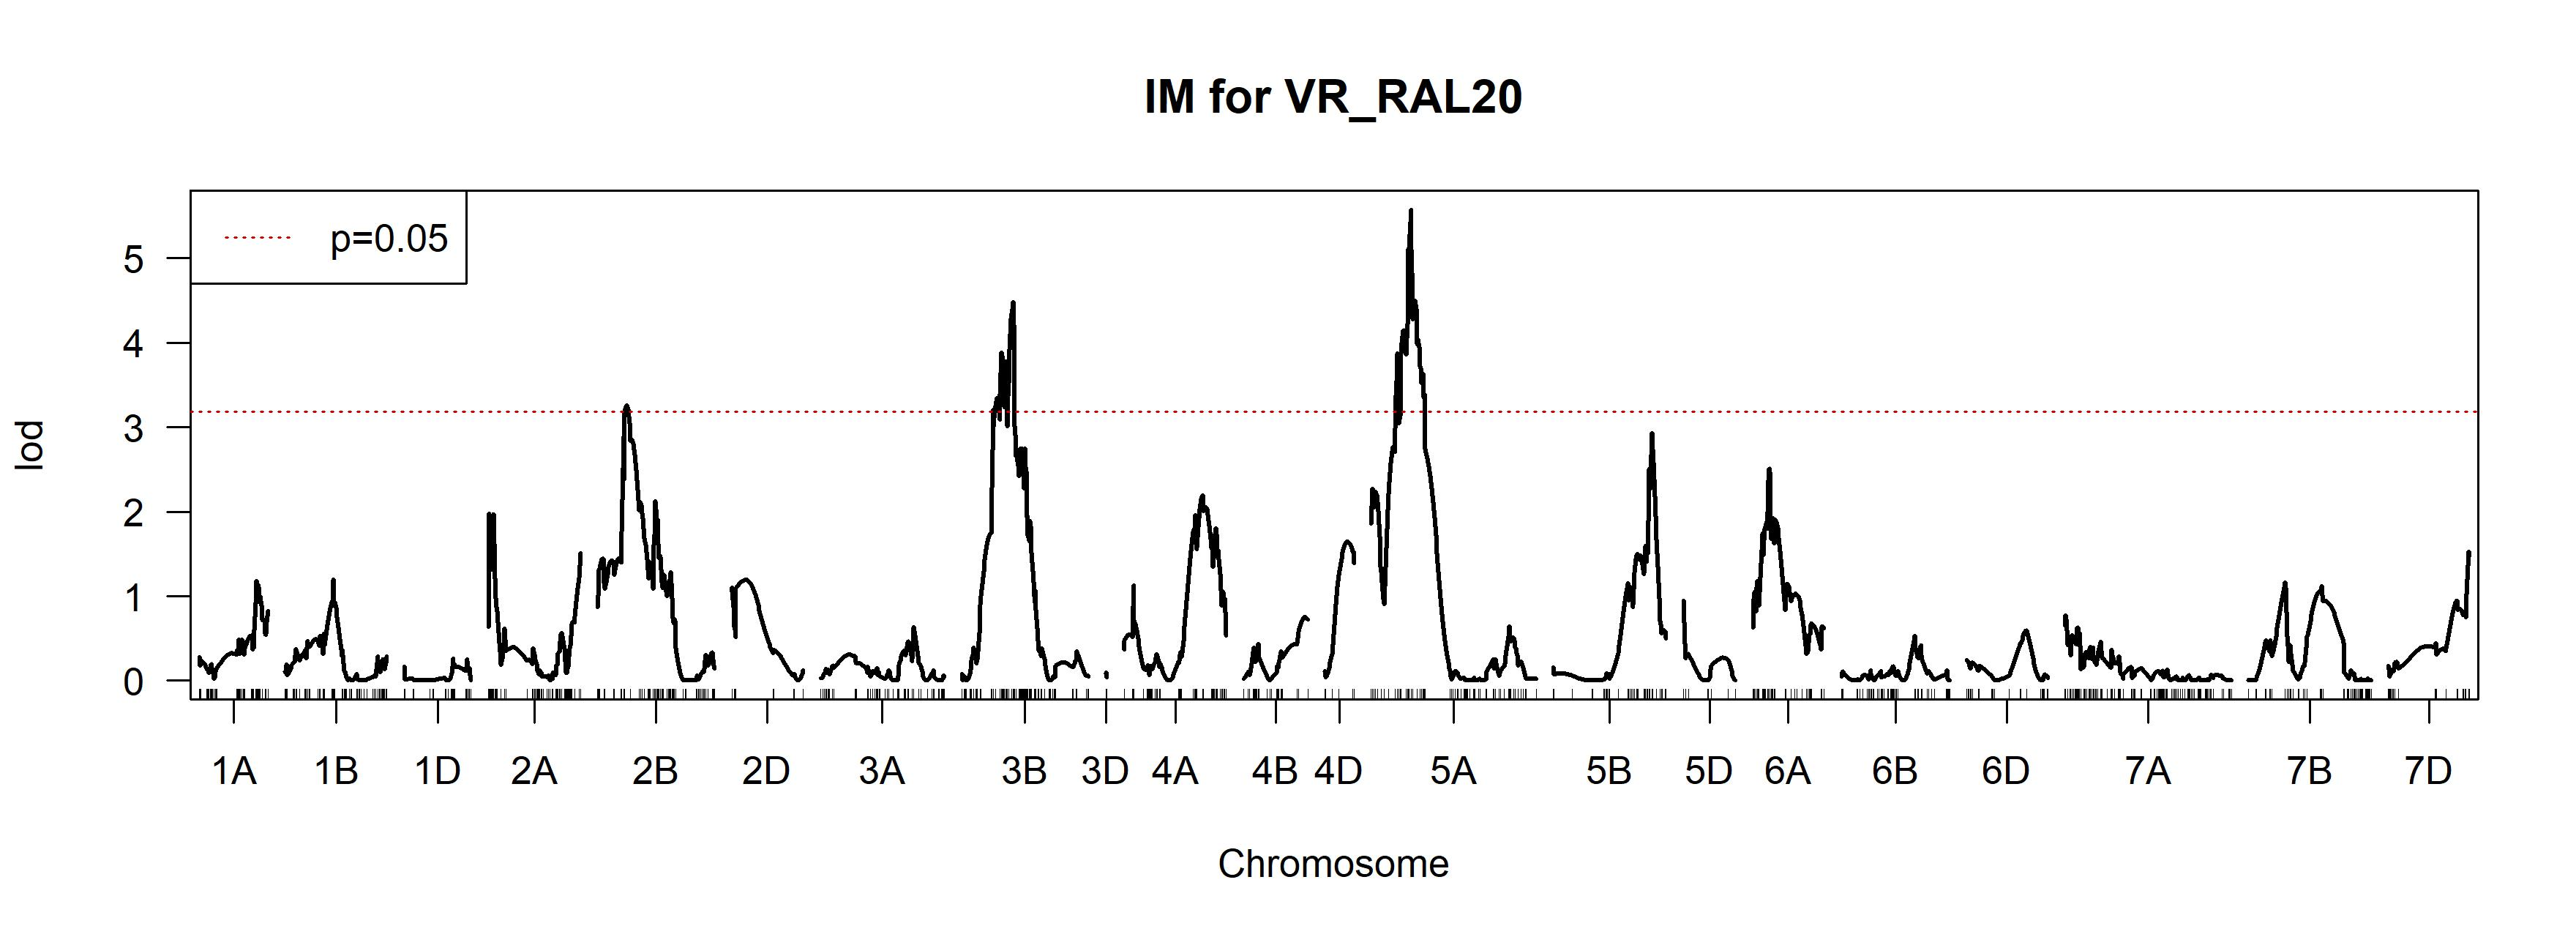
\includegraphics{Scan_IM_VR_RAL20.jpg}
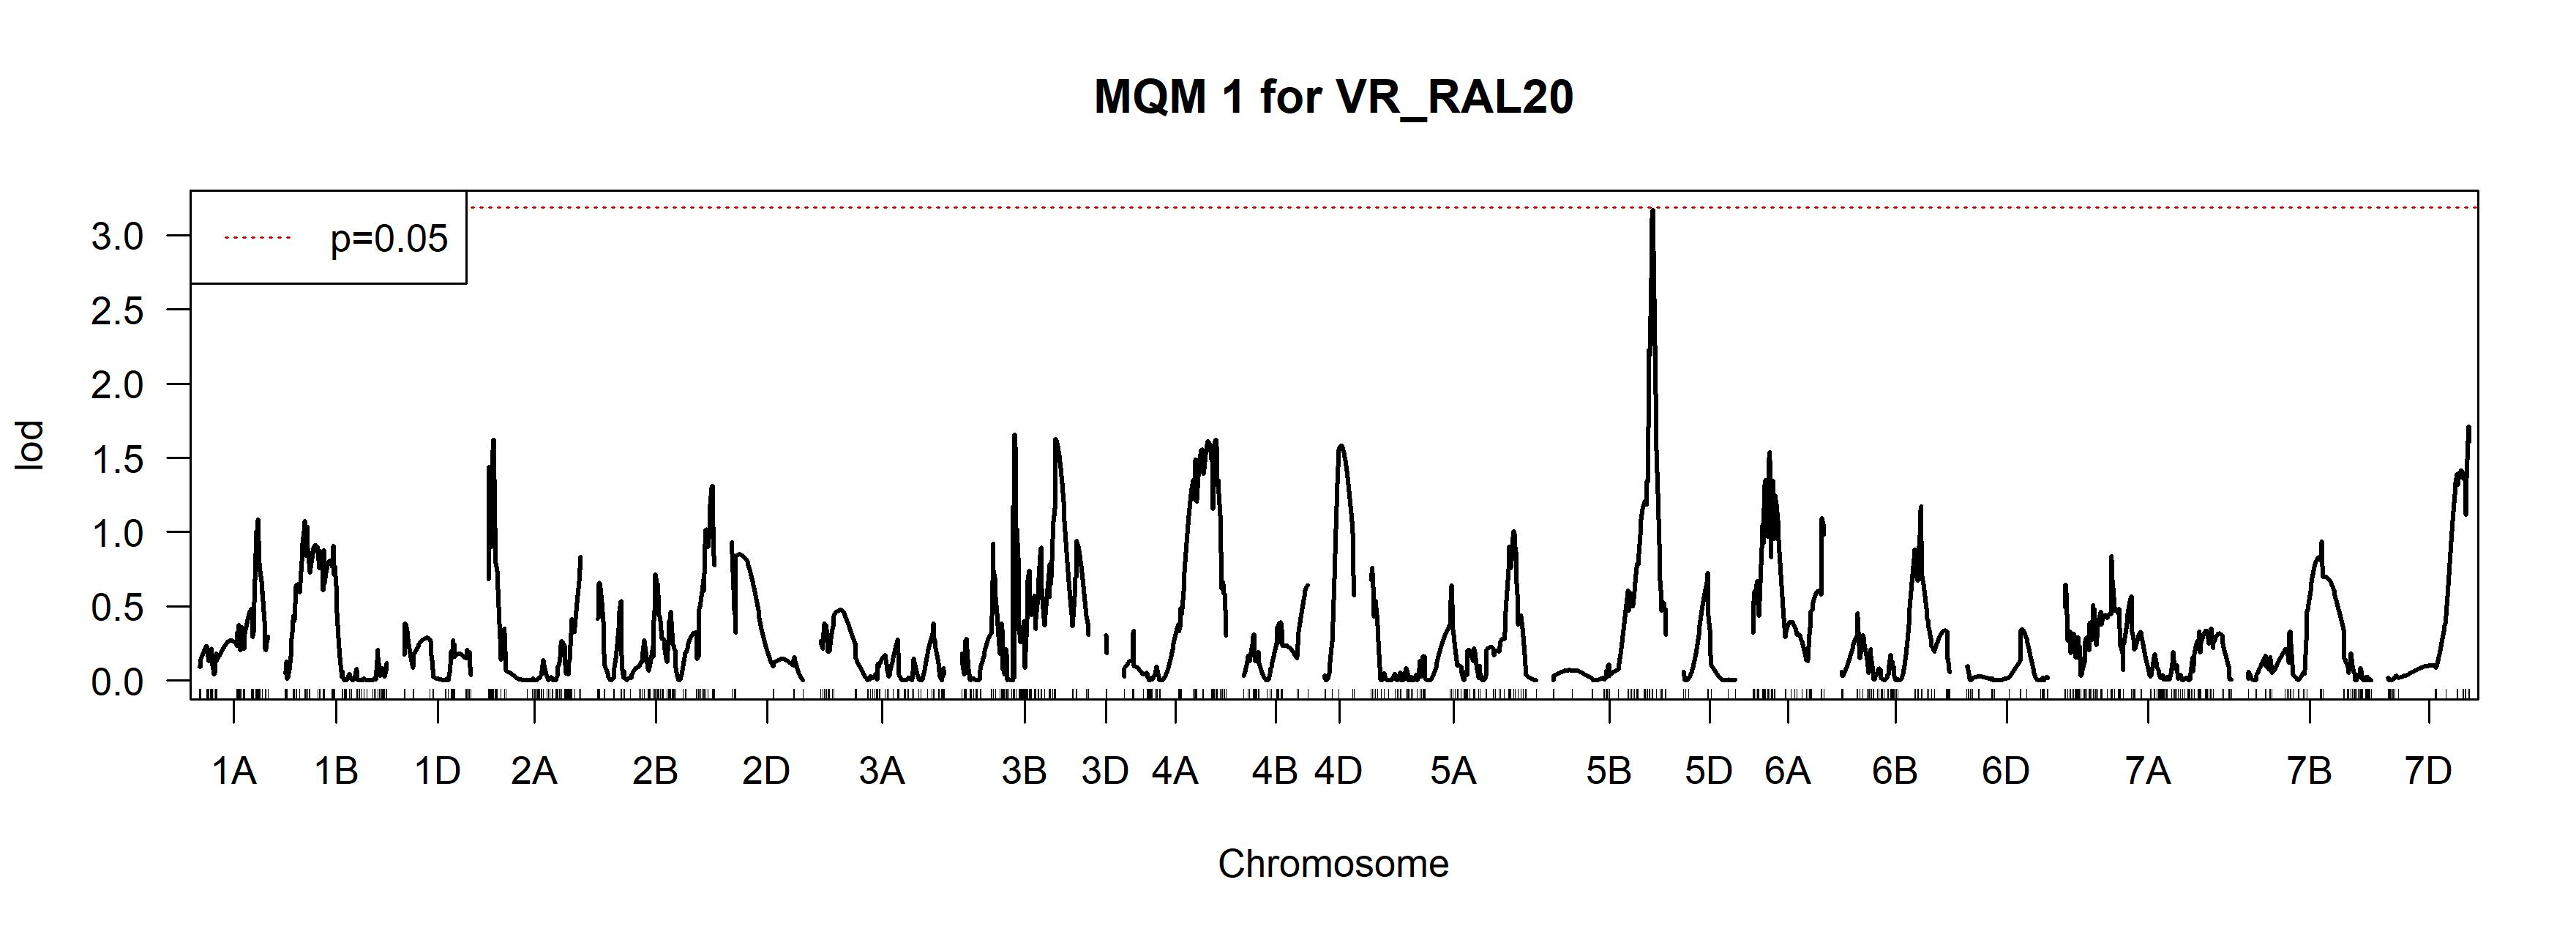
\includegraphics{Scan_MQM1_VR_RAL20.jpg}
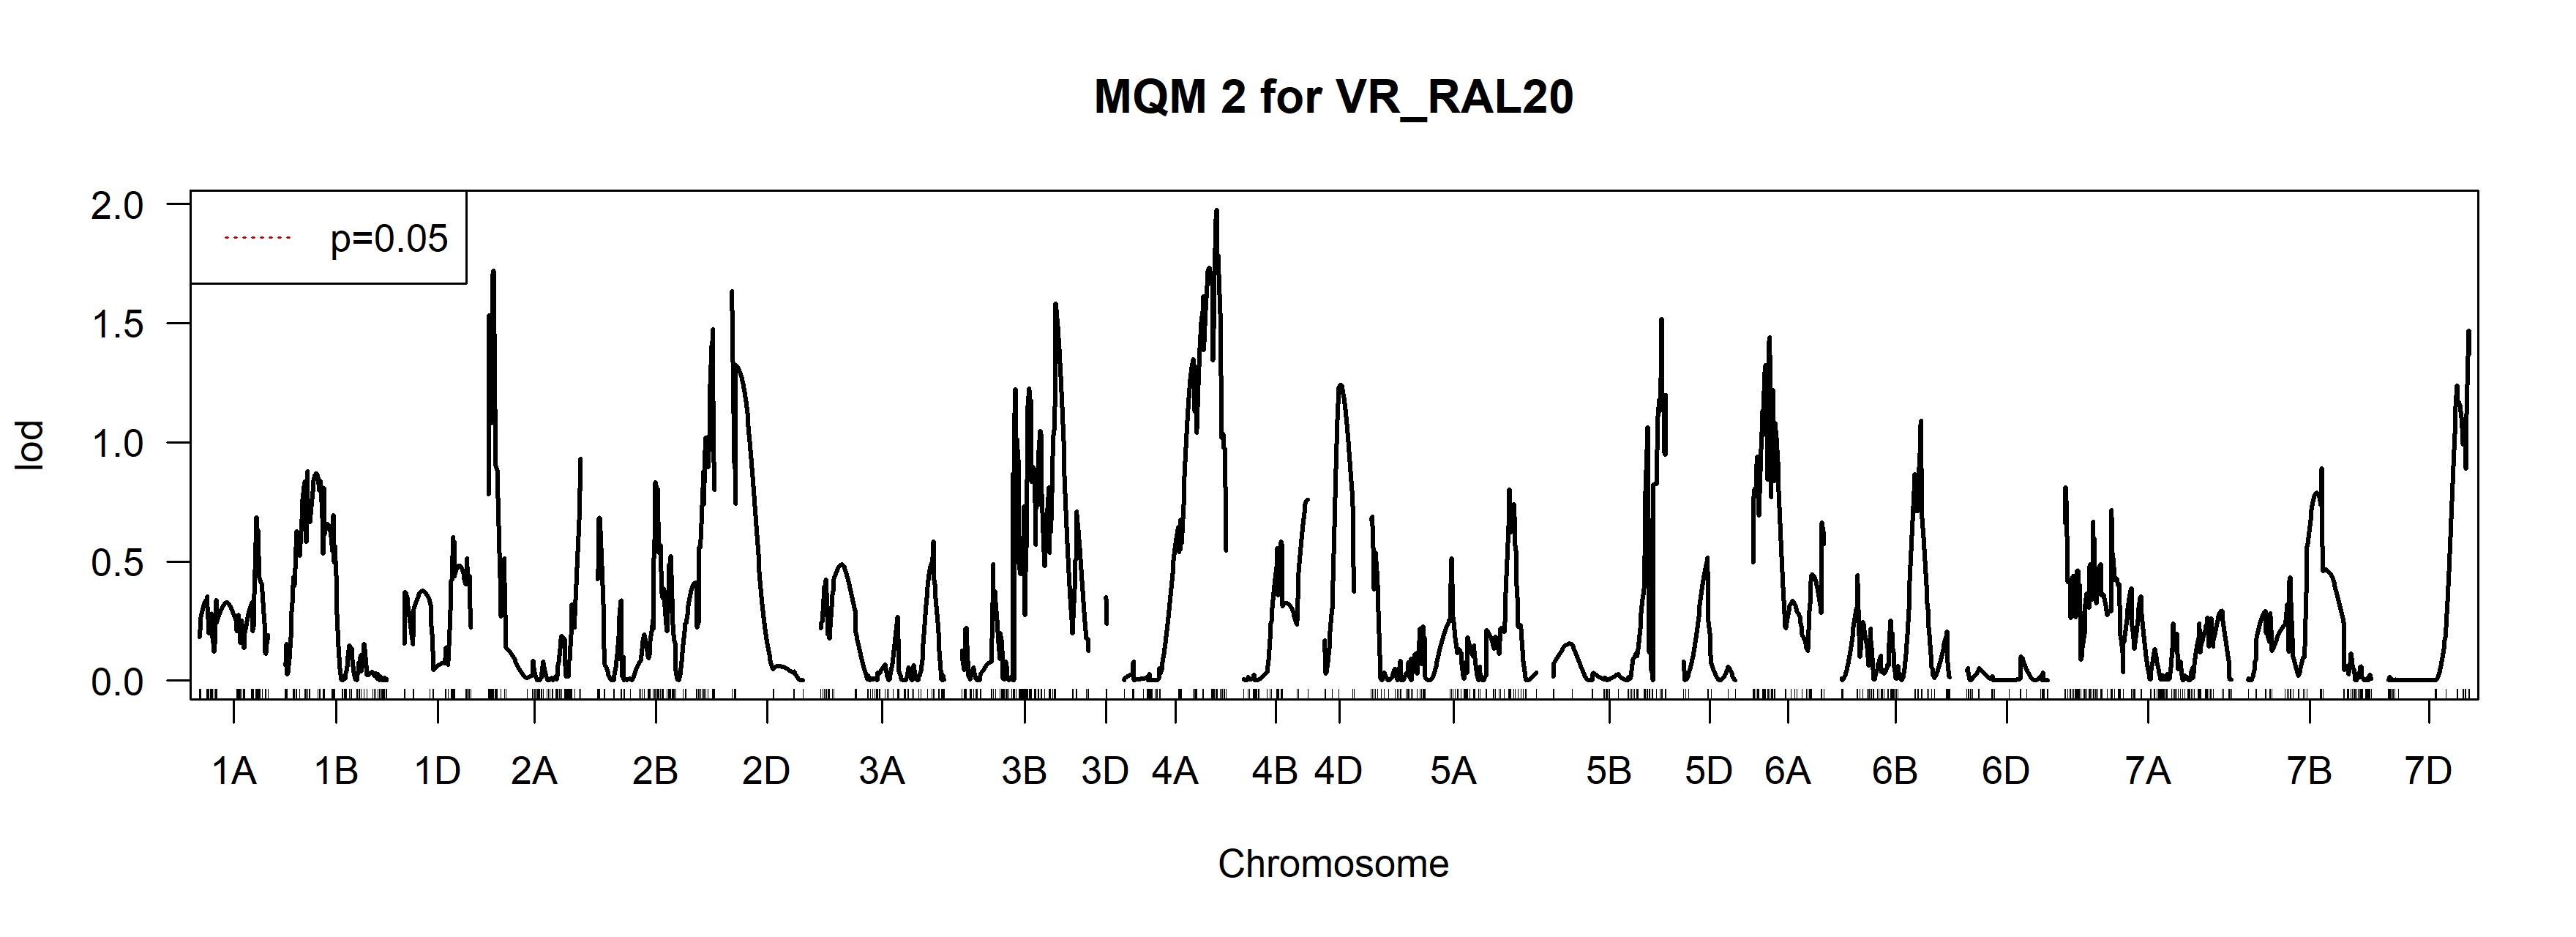
\includegraphics{Scan_MQM2_VR_RAL20.jpg} \pagebreak

\subsection{Visual Ratings in Warsaw, VA -
2020}\label{visual-ratings-in-warsaw-va---2020}

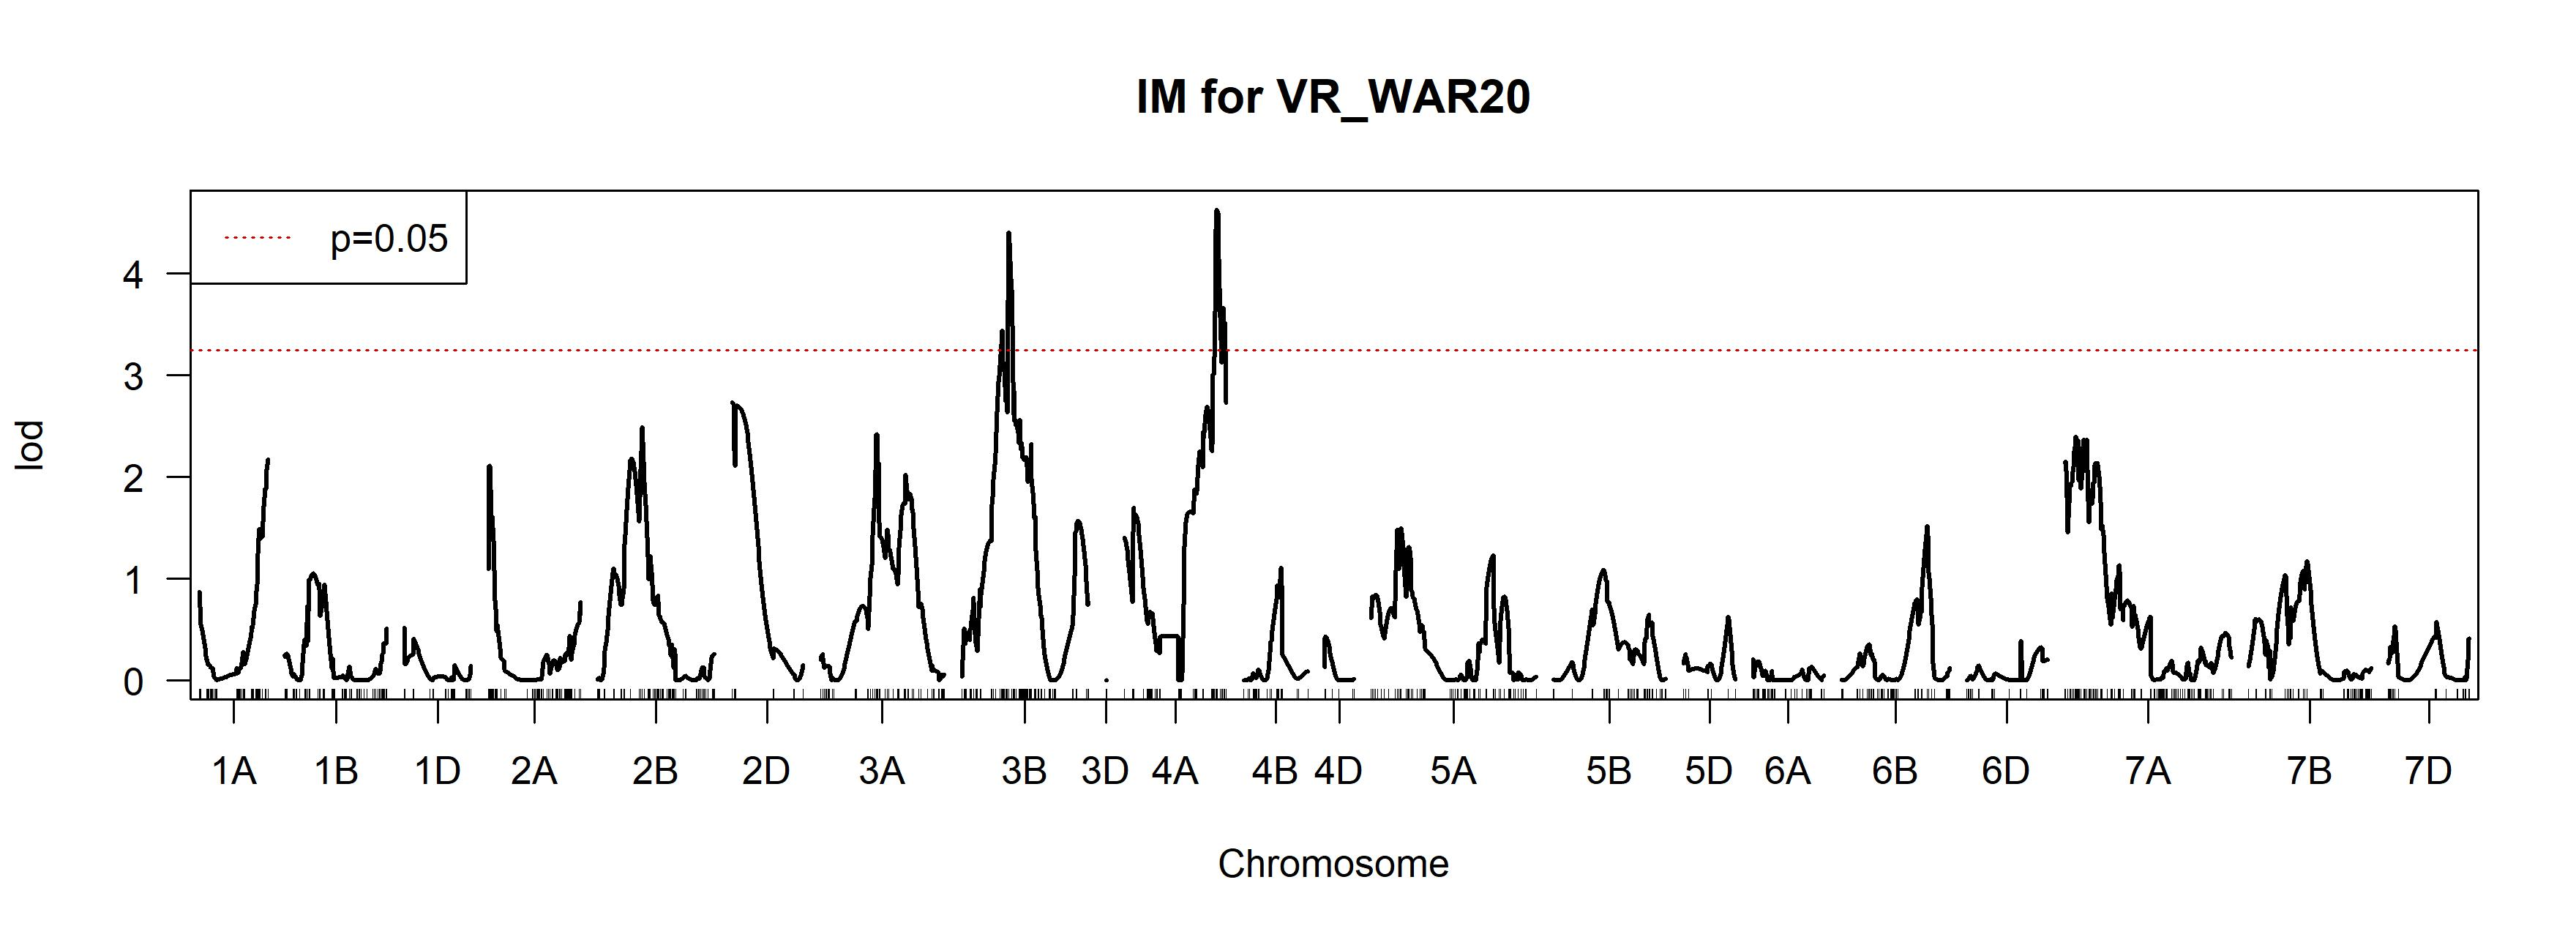
\includegraphics{Scan_IM_VR_WAR20.jpg}
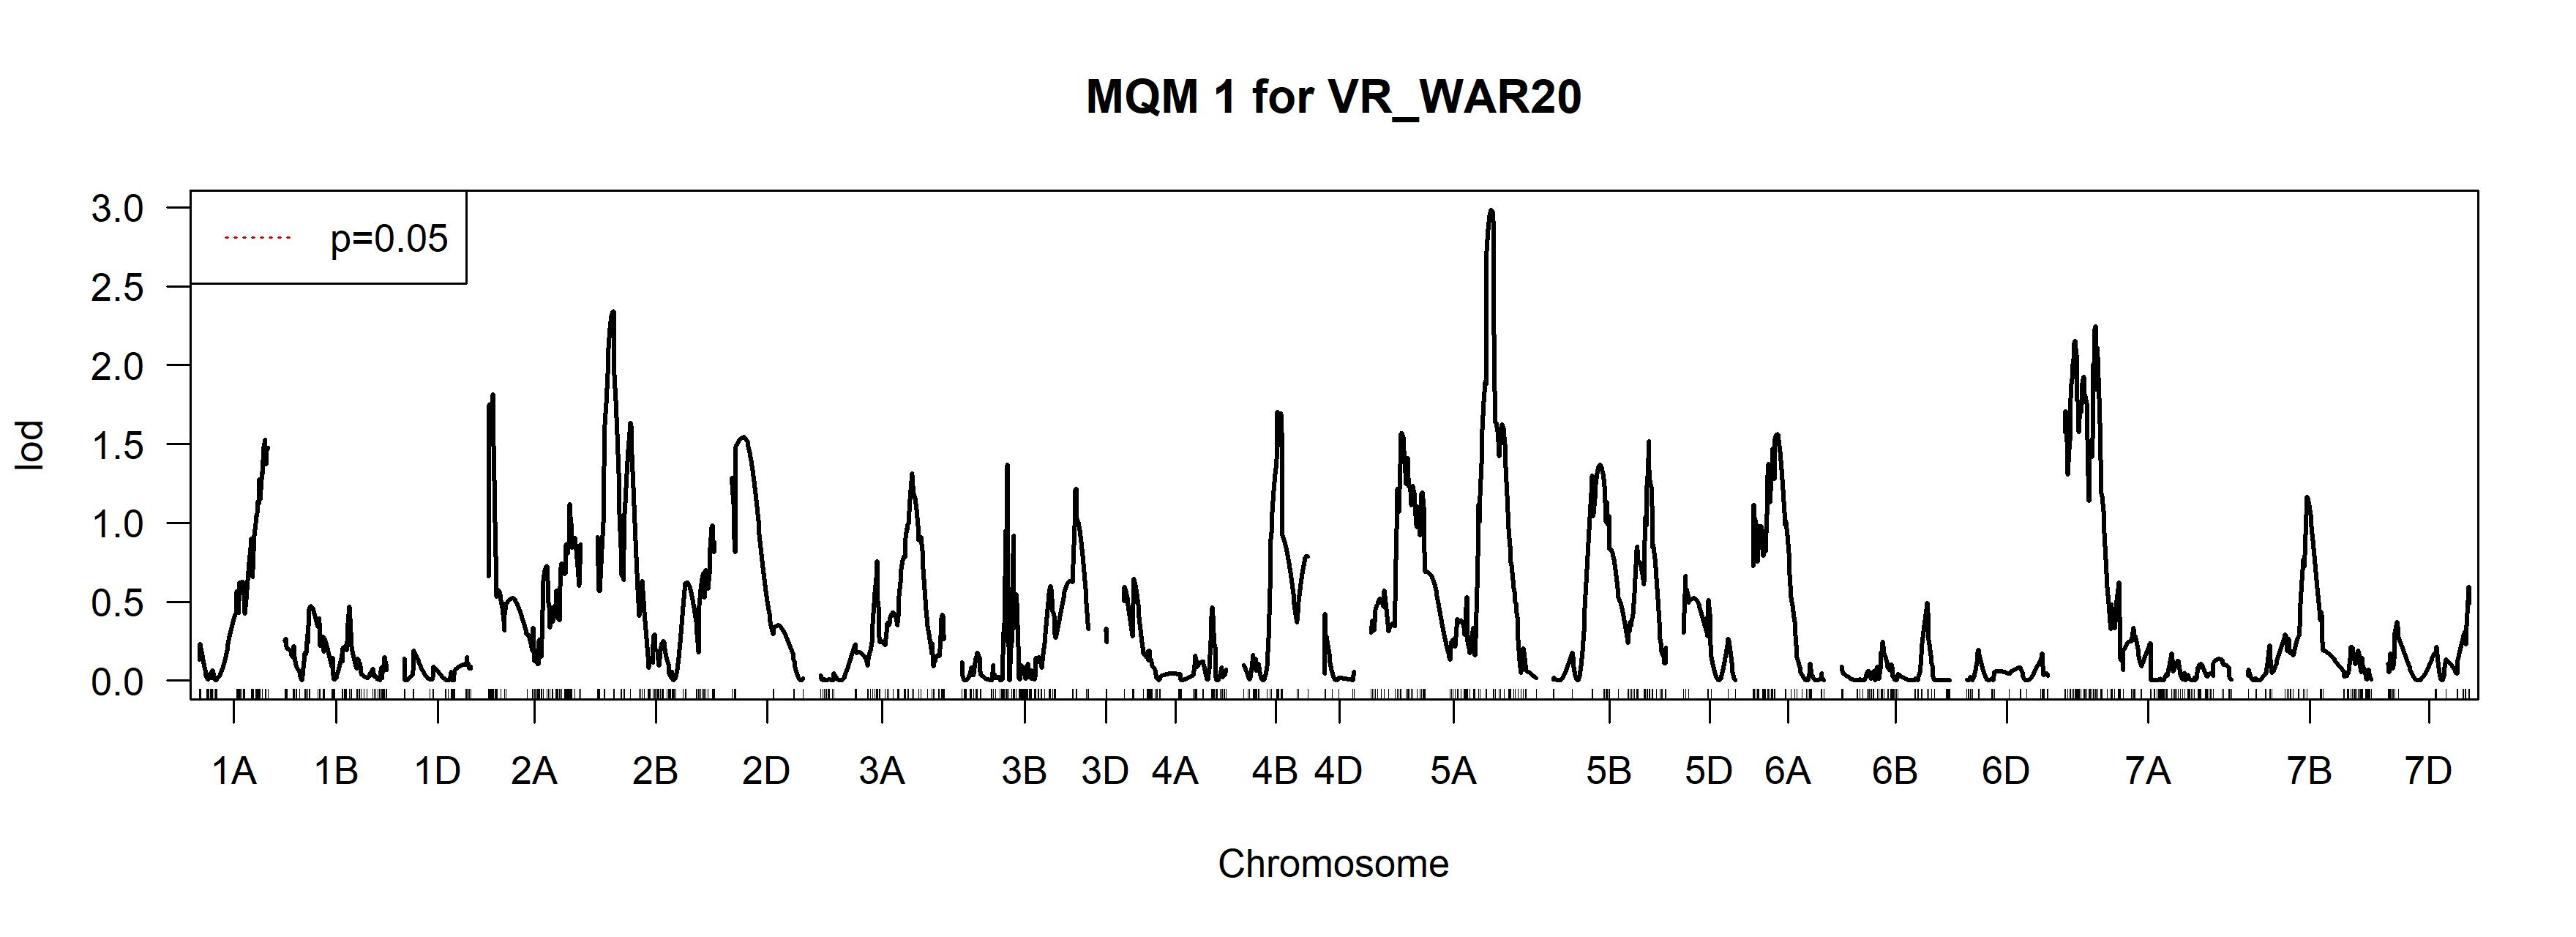
\includegraphics{Scan_MQM1_VR_WAR20.jpg} \pagebreak

\subsection{Fusarium Damaged Kernels Across All
Environments}\label{fusarium-damaged-kernels-across-all-environments}

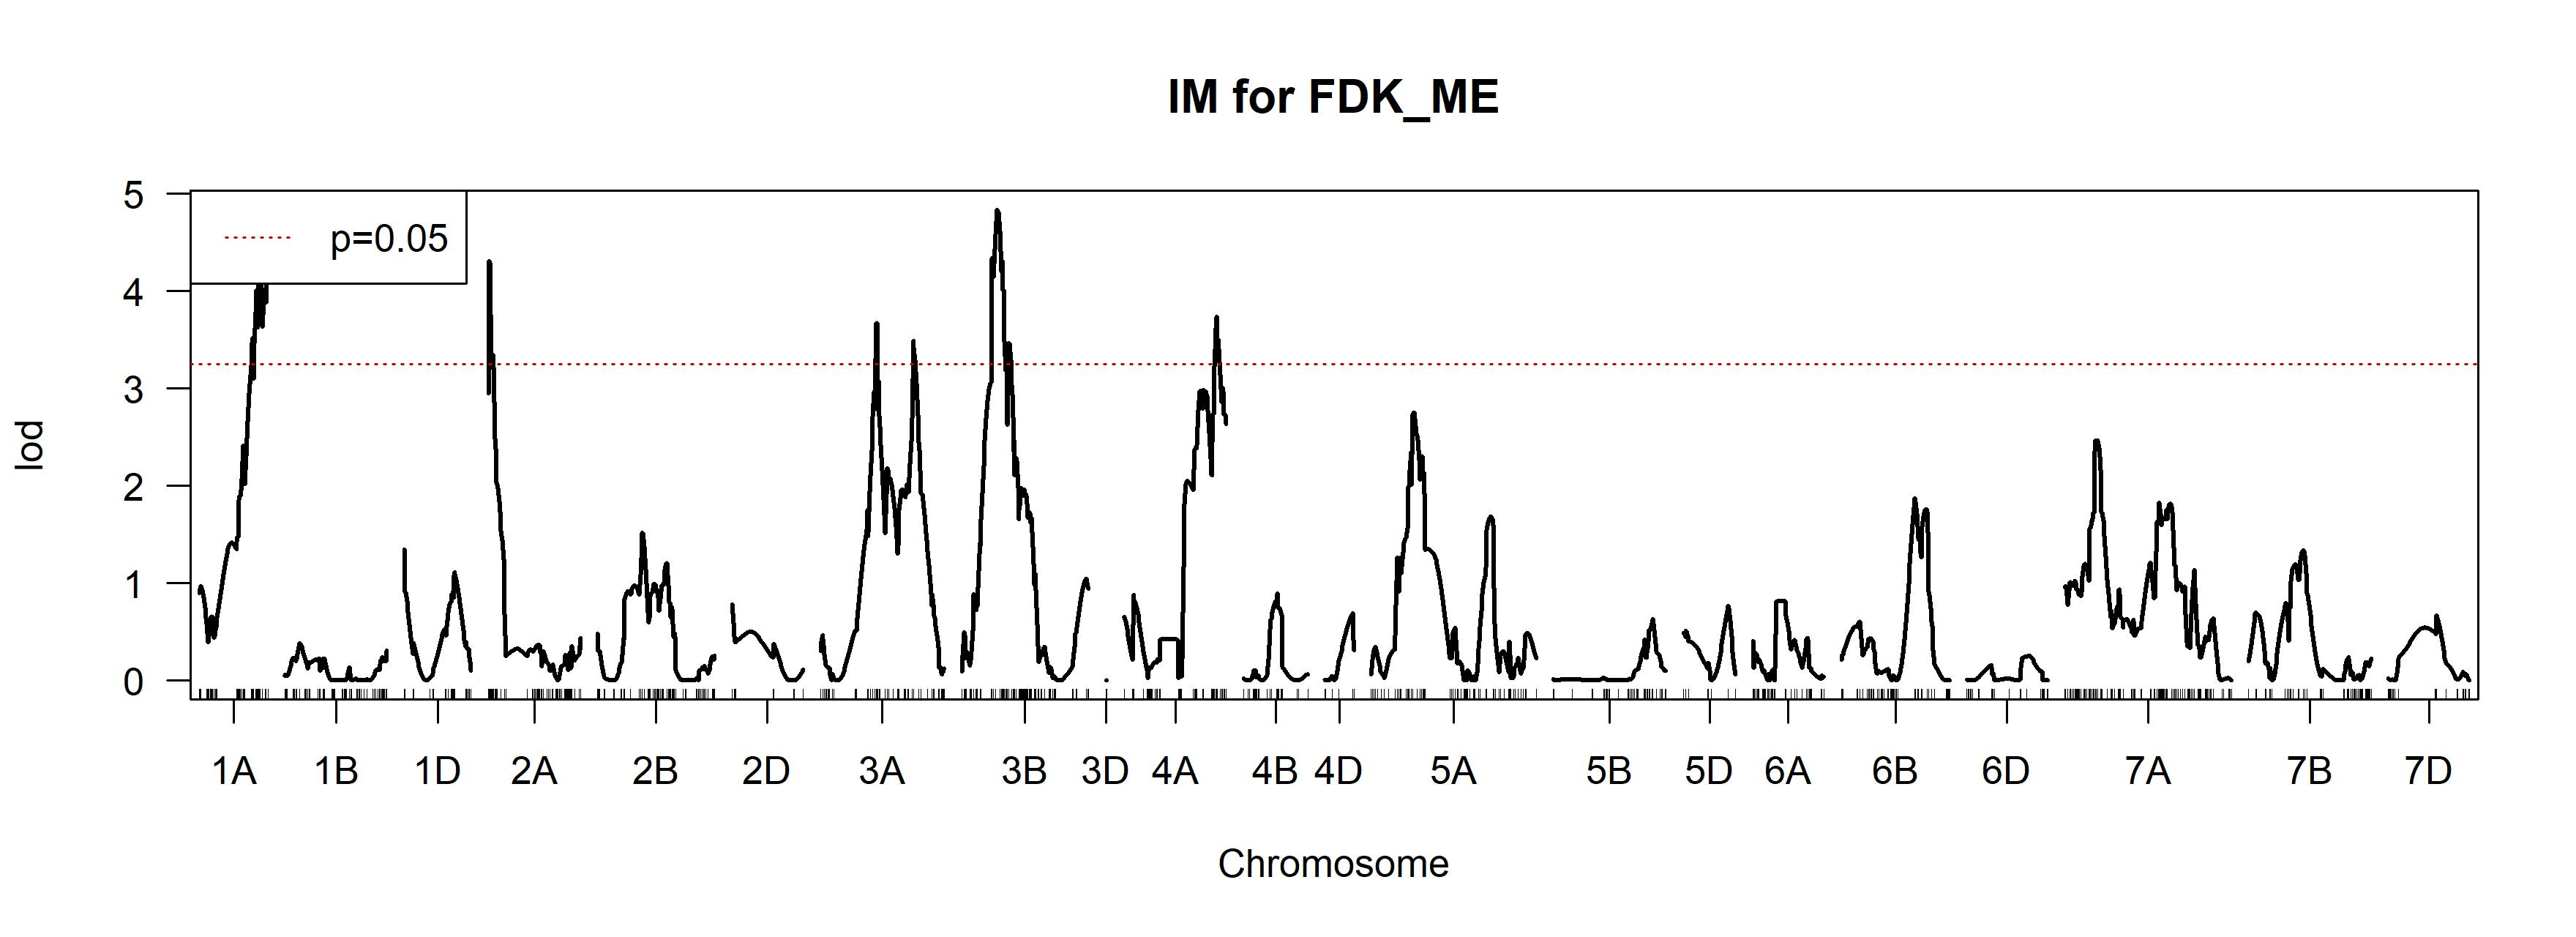
\includegraphics{Scan_IM_FDK_ME.jpg}
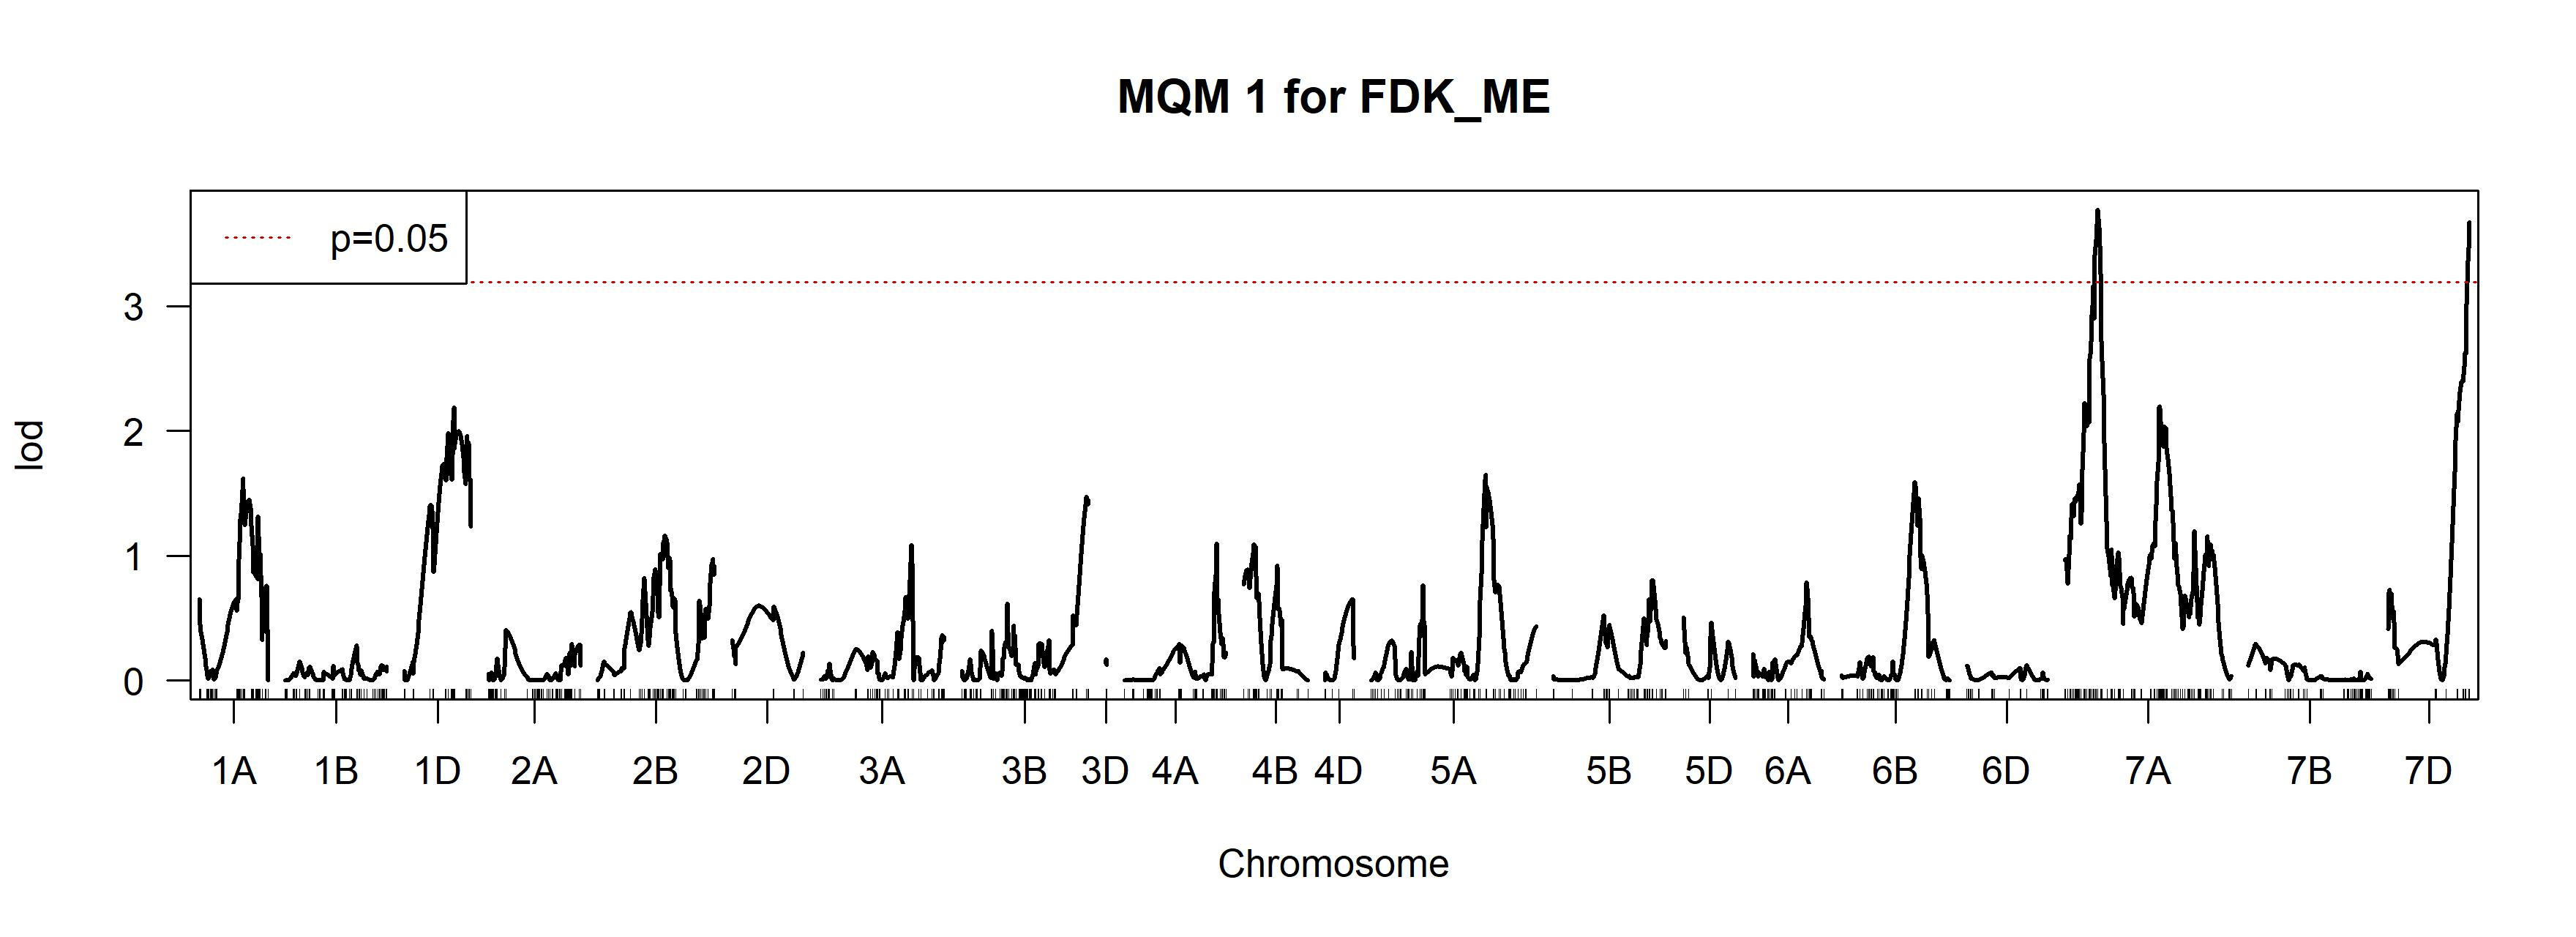
\includegraphics{Scan_MQM1_FDK_ME.jpg}
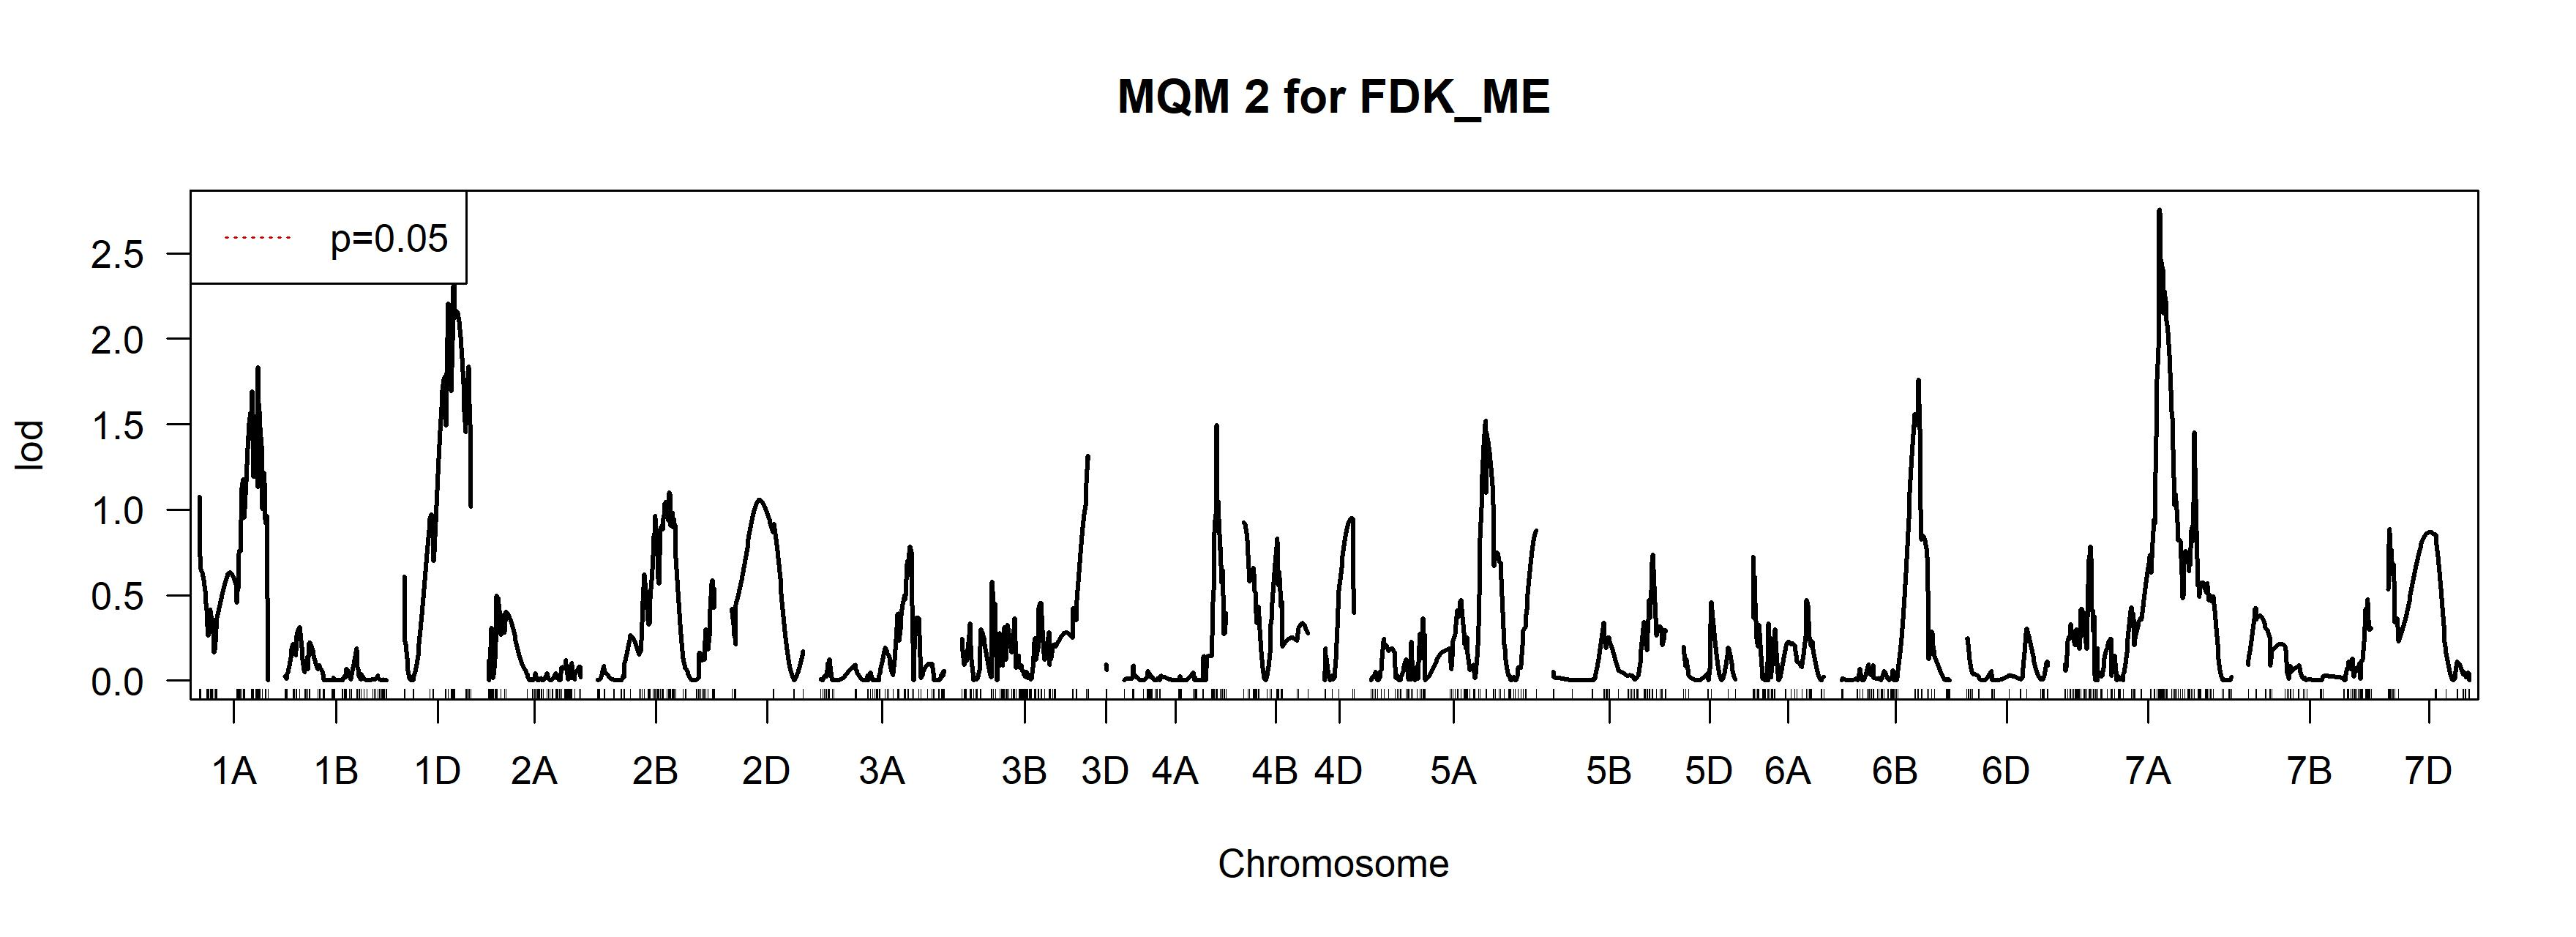
\includegraphics{Scan_MQM2_FDK_ME.jpg} \pagebreak

\subsection{Fusarium Damaged Kernels in Kinston, NC -
2019}\label{fusarium-damaged-kernels-in-kinston-nc---2019}

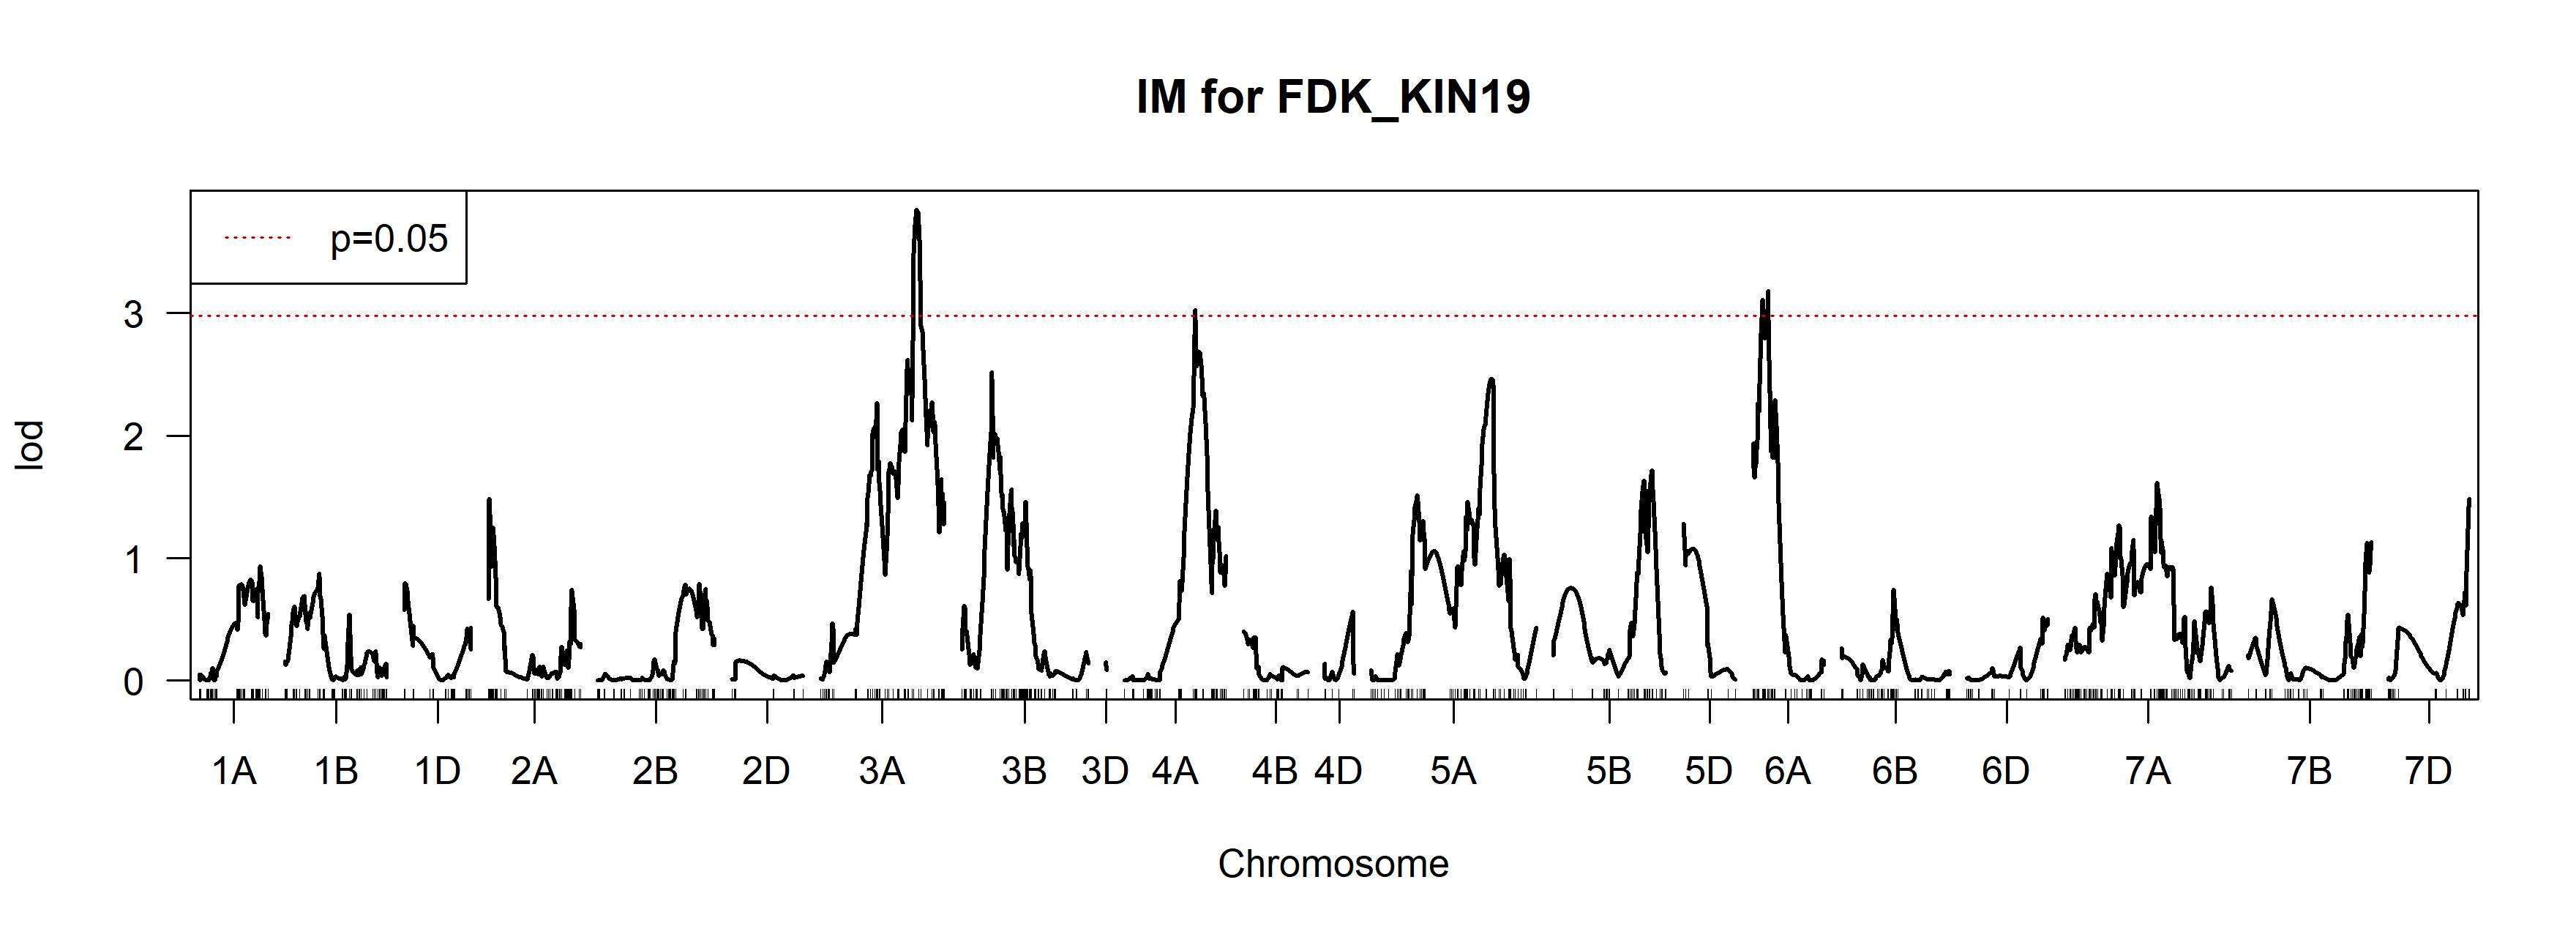
\includegraphics{Scan_IM_FDK_KIN19.jpg}
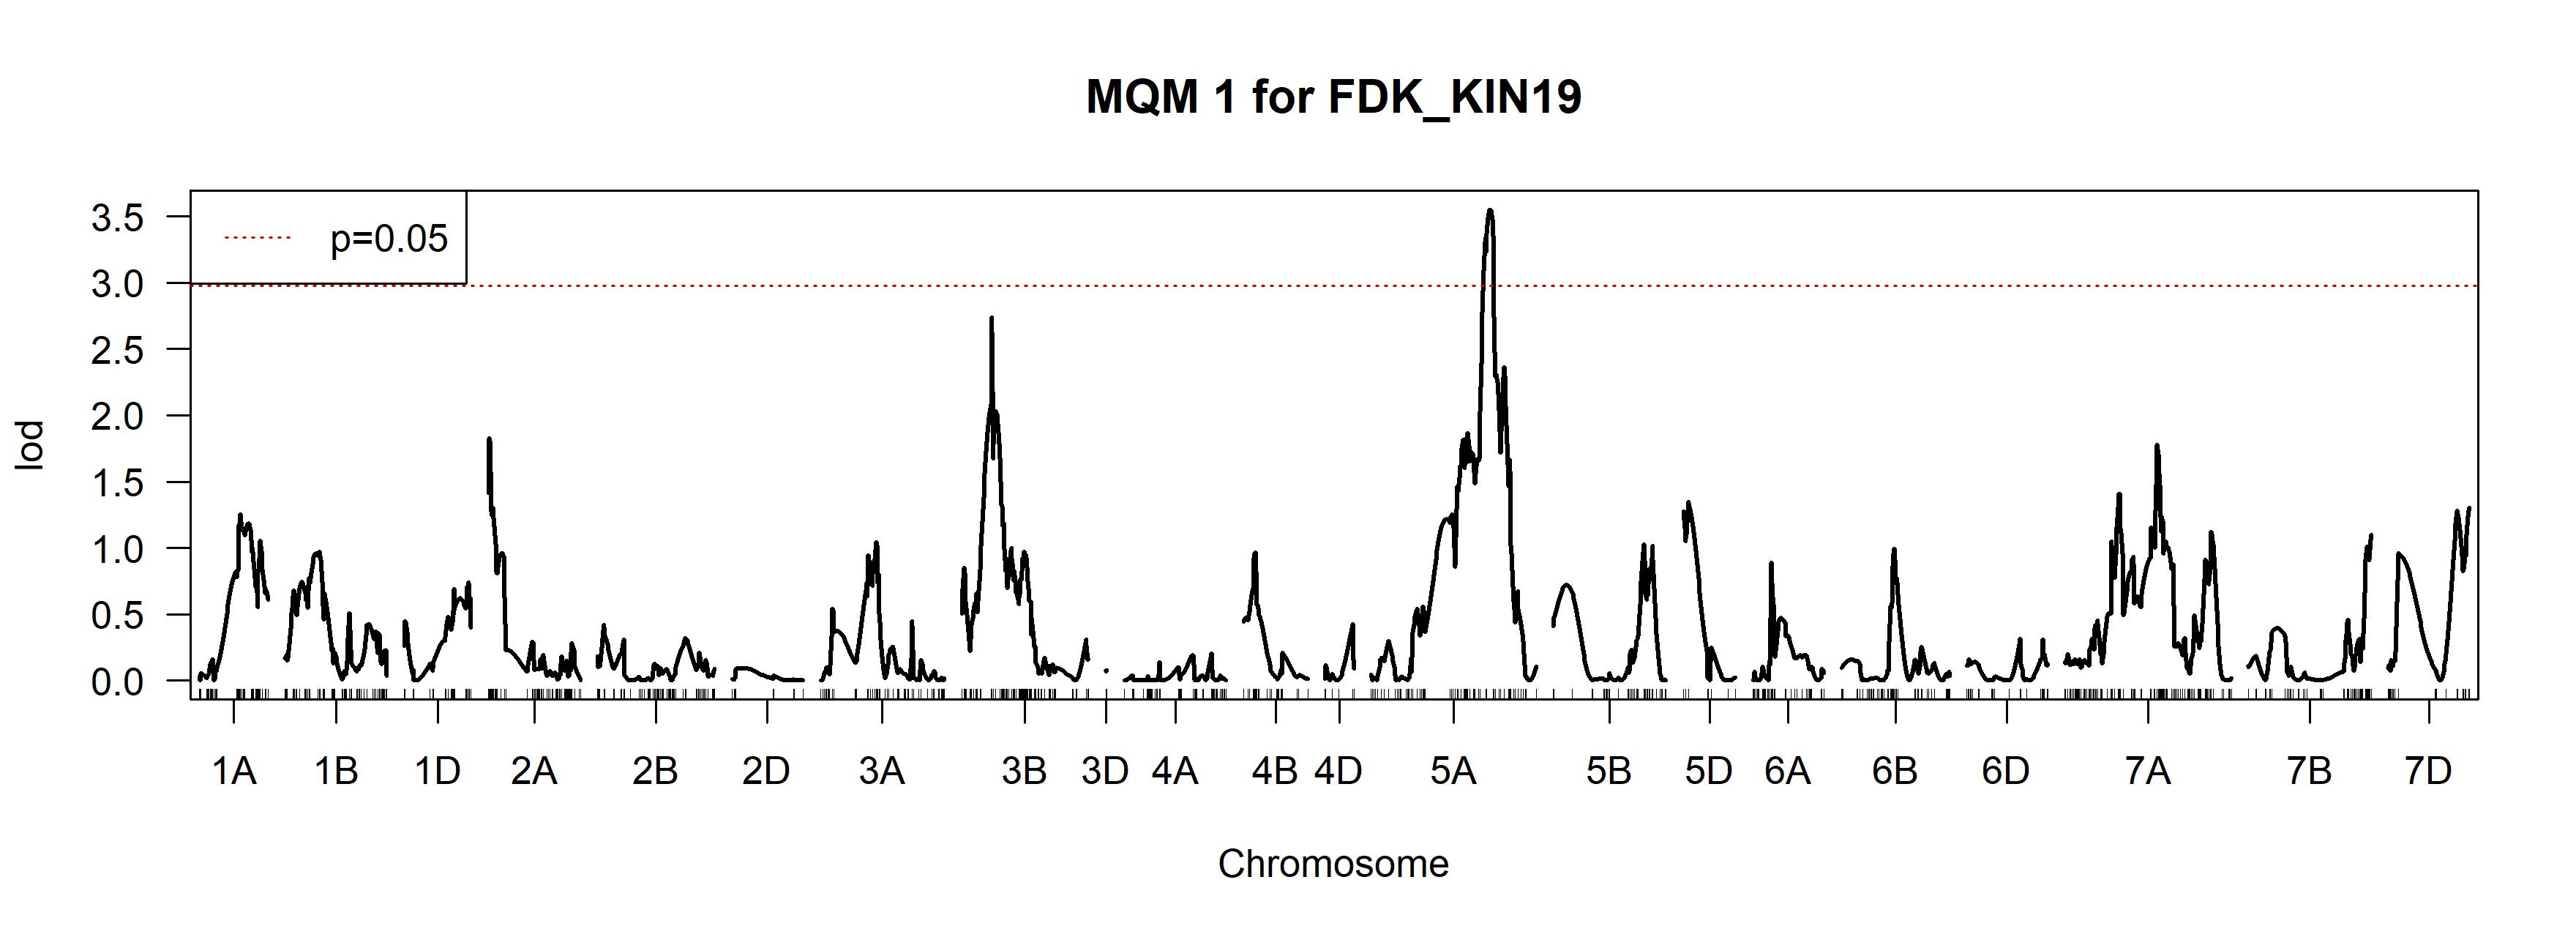
\includegraphics{Scan_MQM1_FDK_KIN19.jpg}
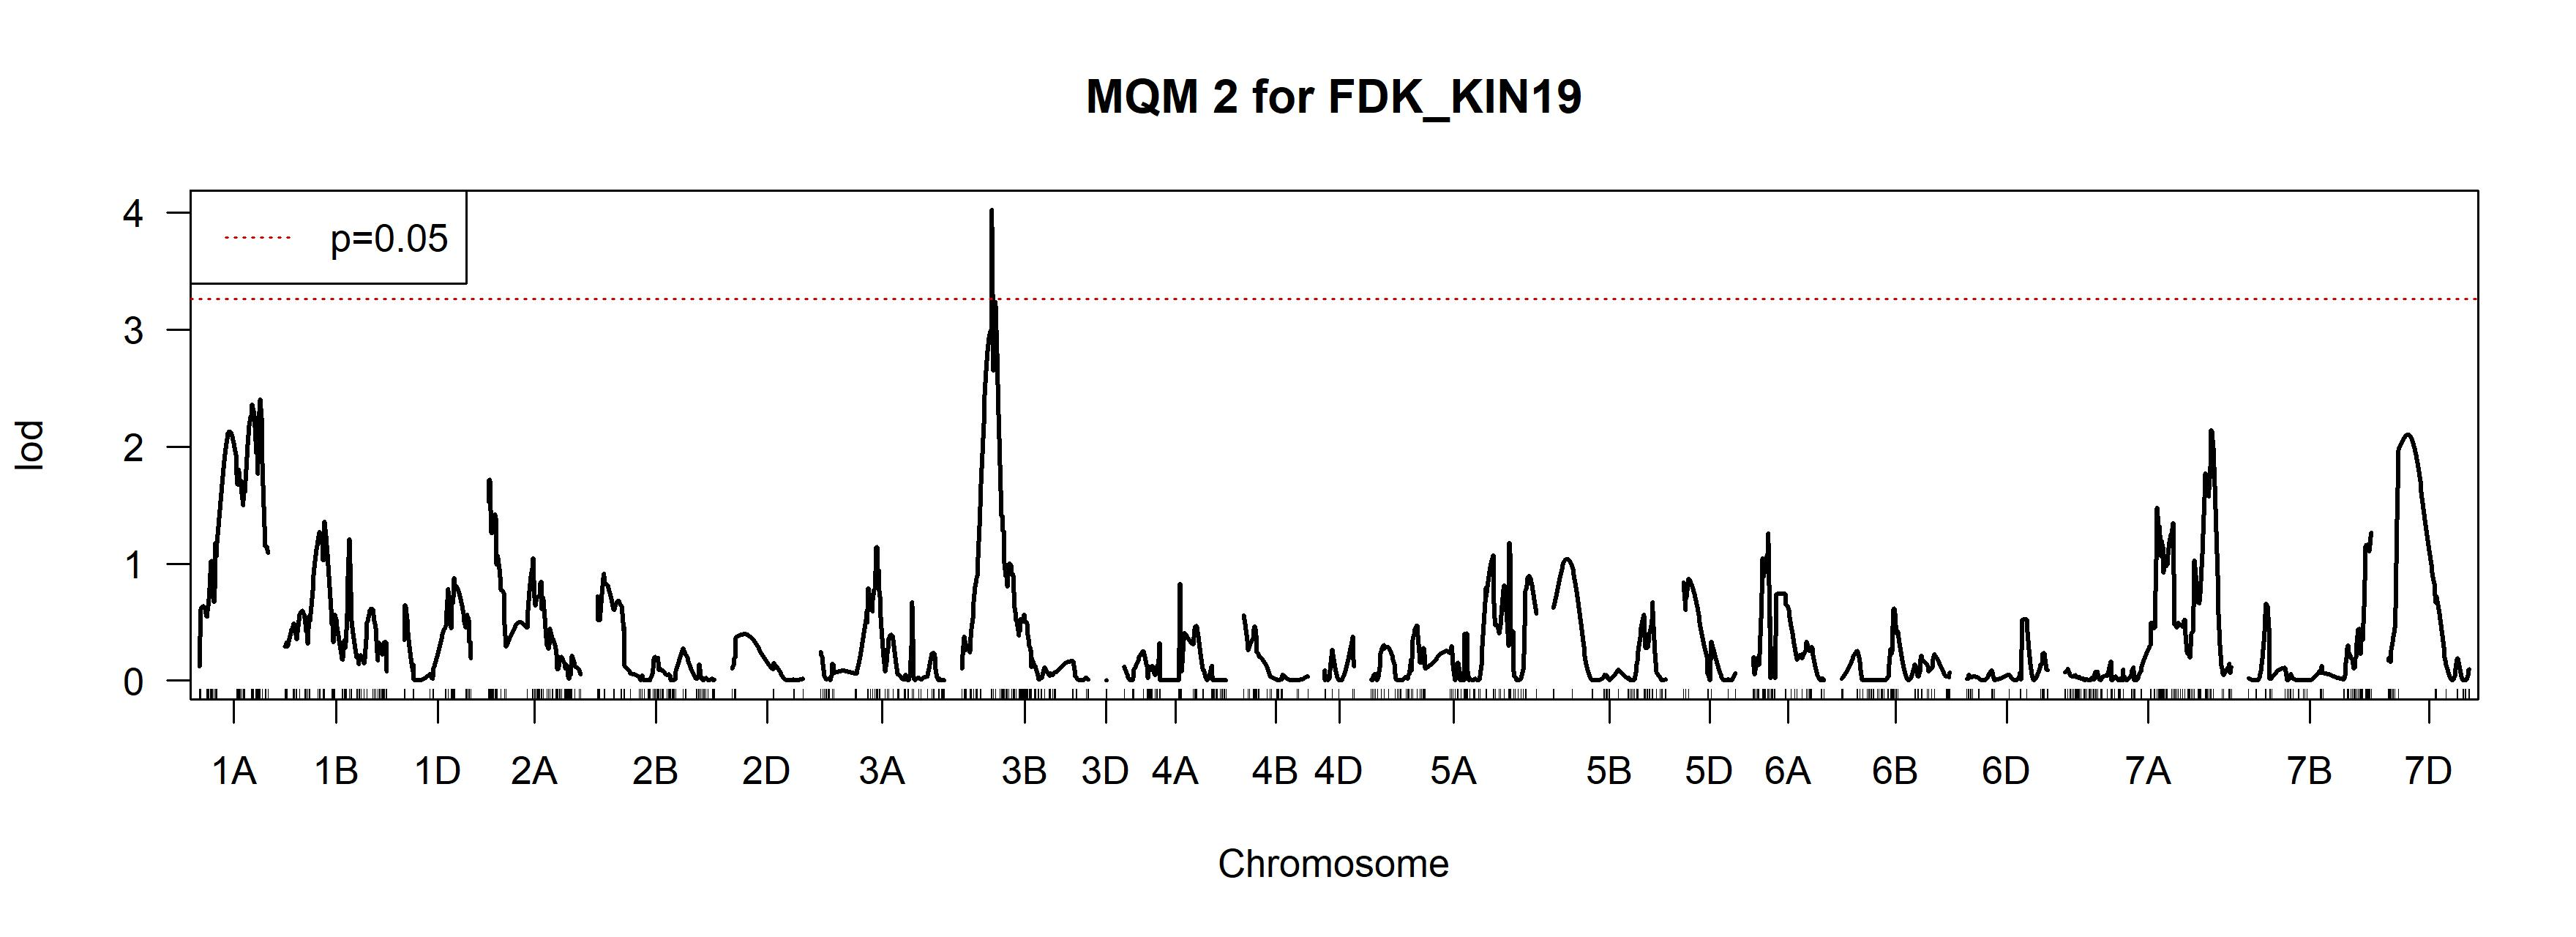
\includegraphics{Scan_MQM2_FDK_KIN19.jpg}
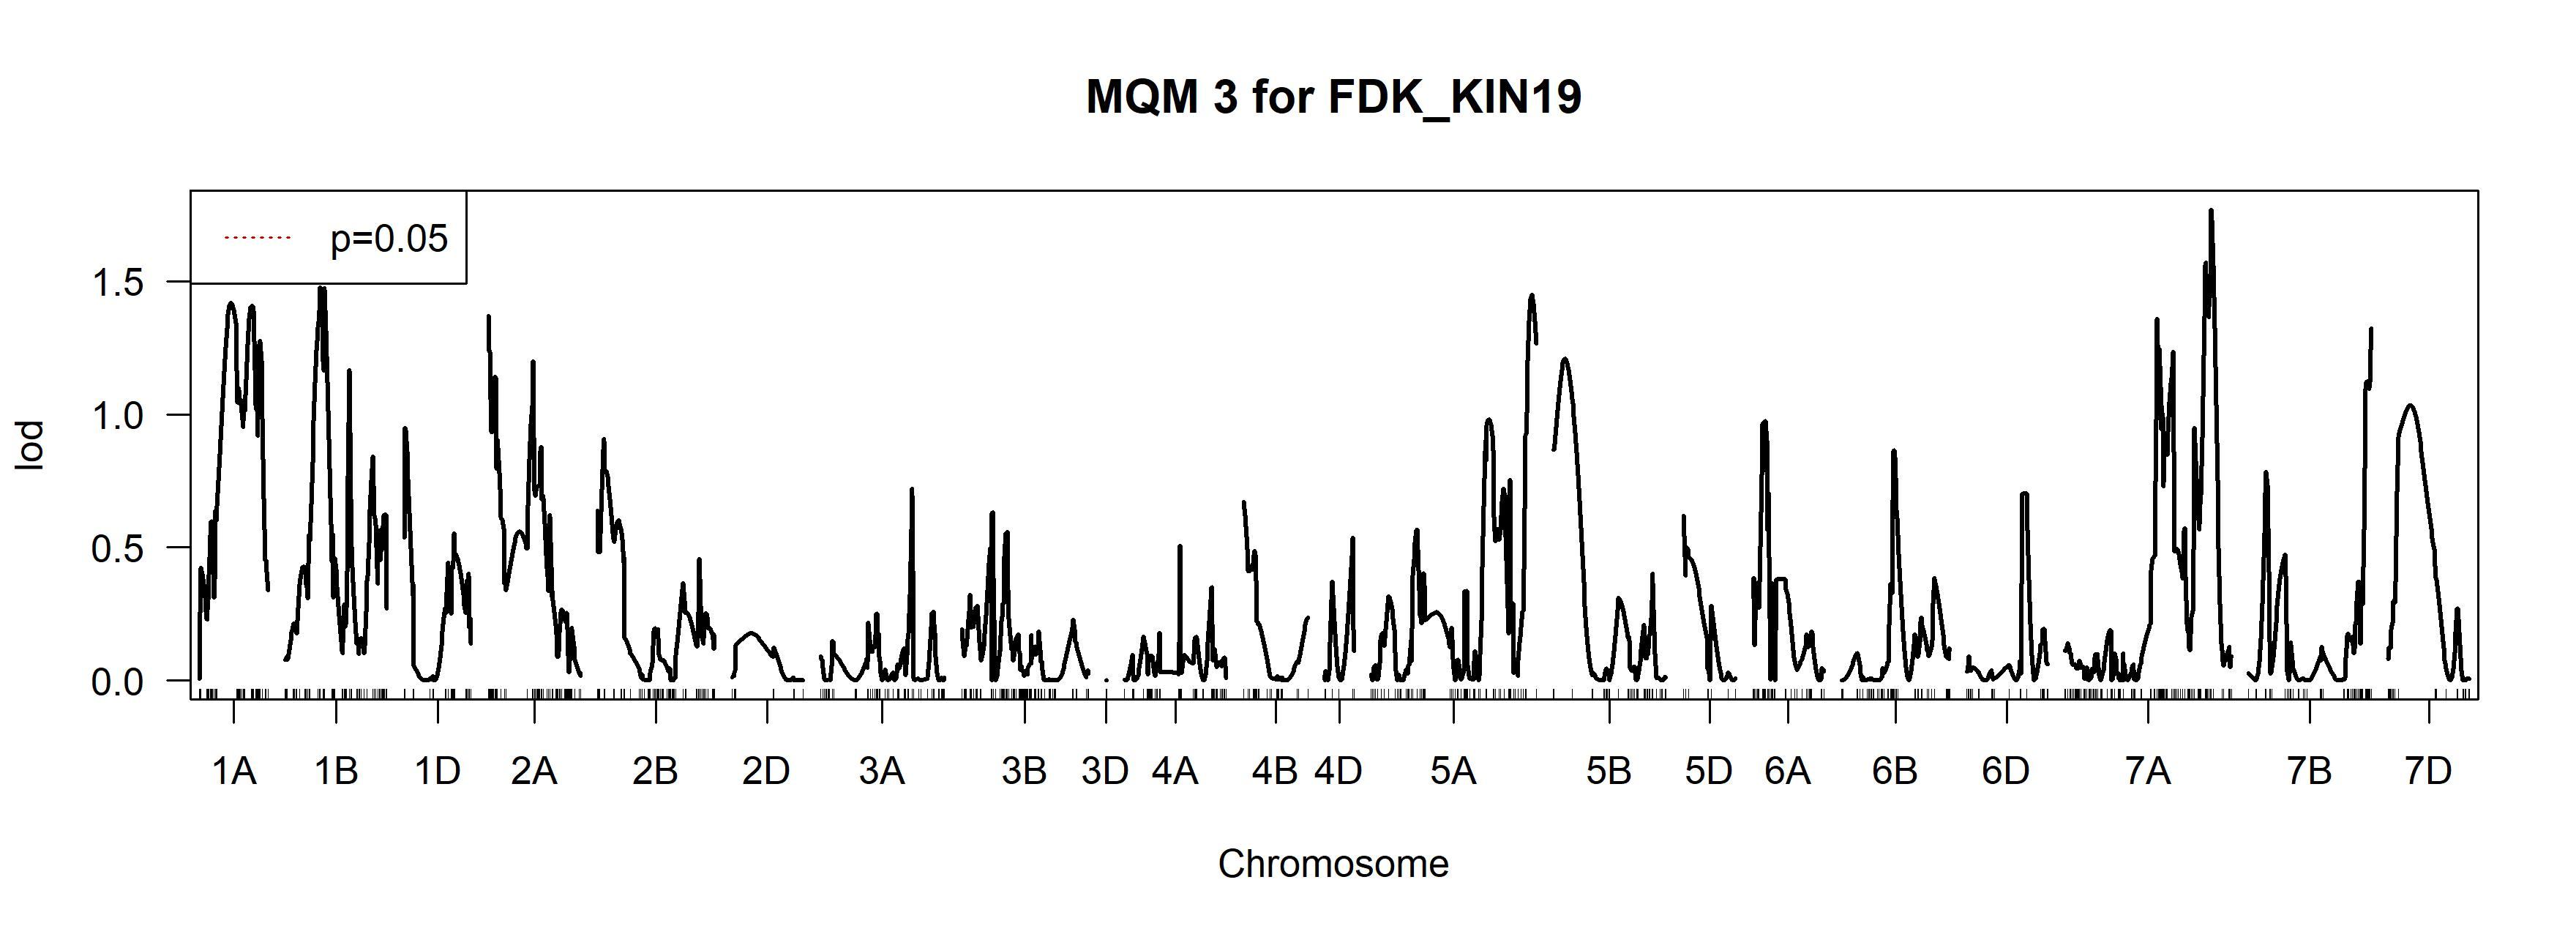
\includegraphics{Scan_MQM3_FDK_KIN19.jpg} \pagebreak

\subsection{Fusarium Damaged Kernels in Kinston, NC -
2020}\label{fusarium-damaged-kernels-in-kinston-nc---2020}

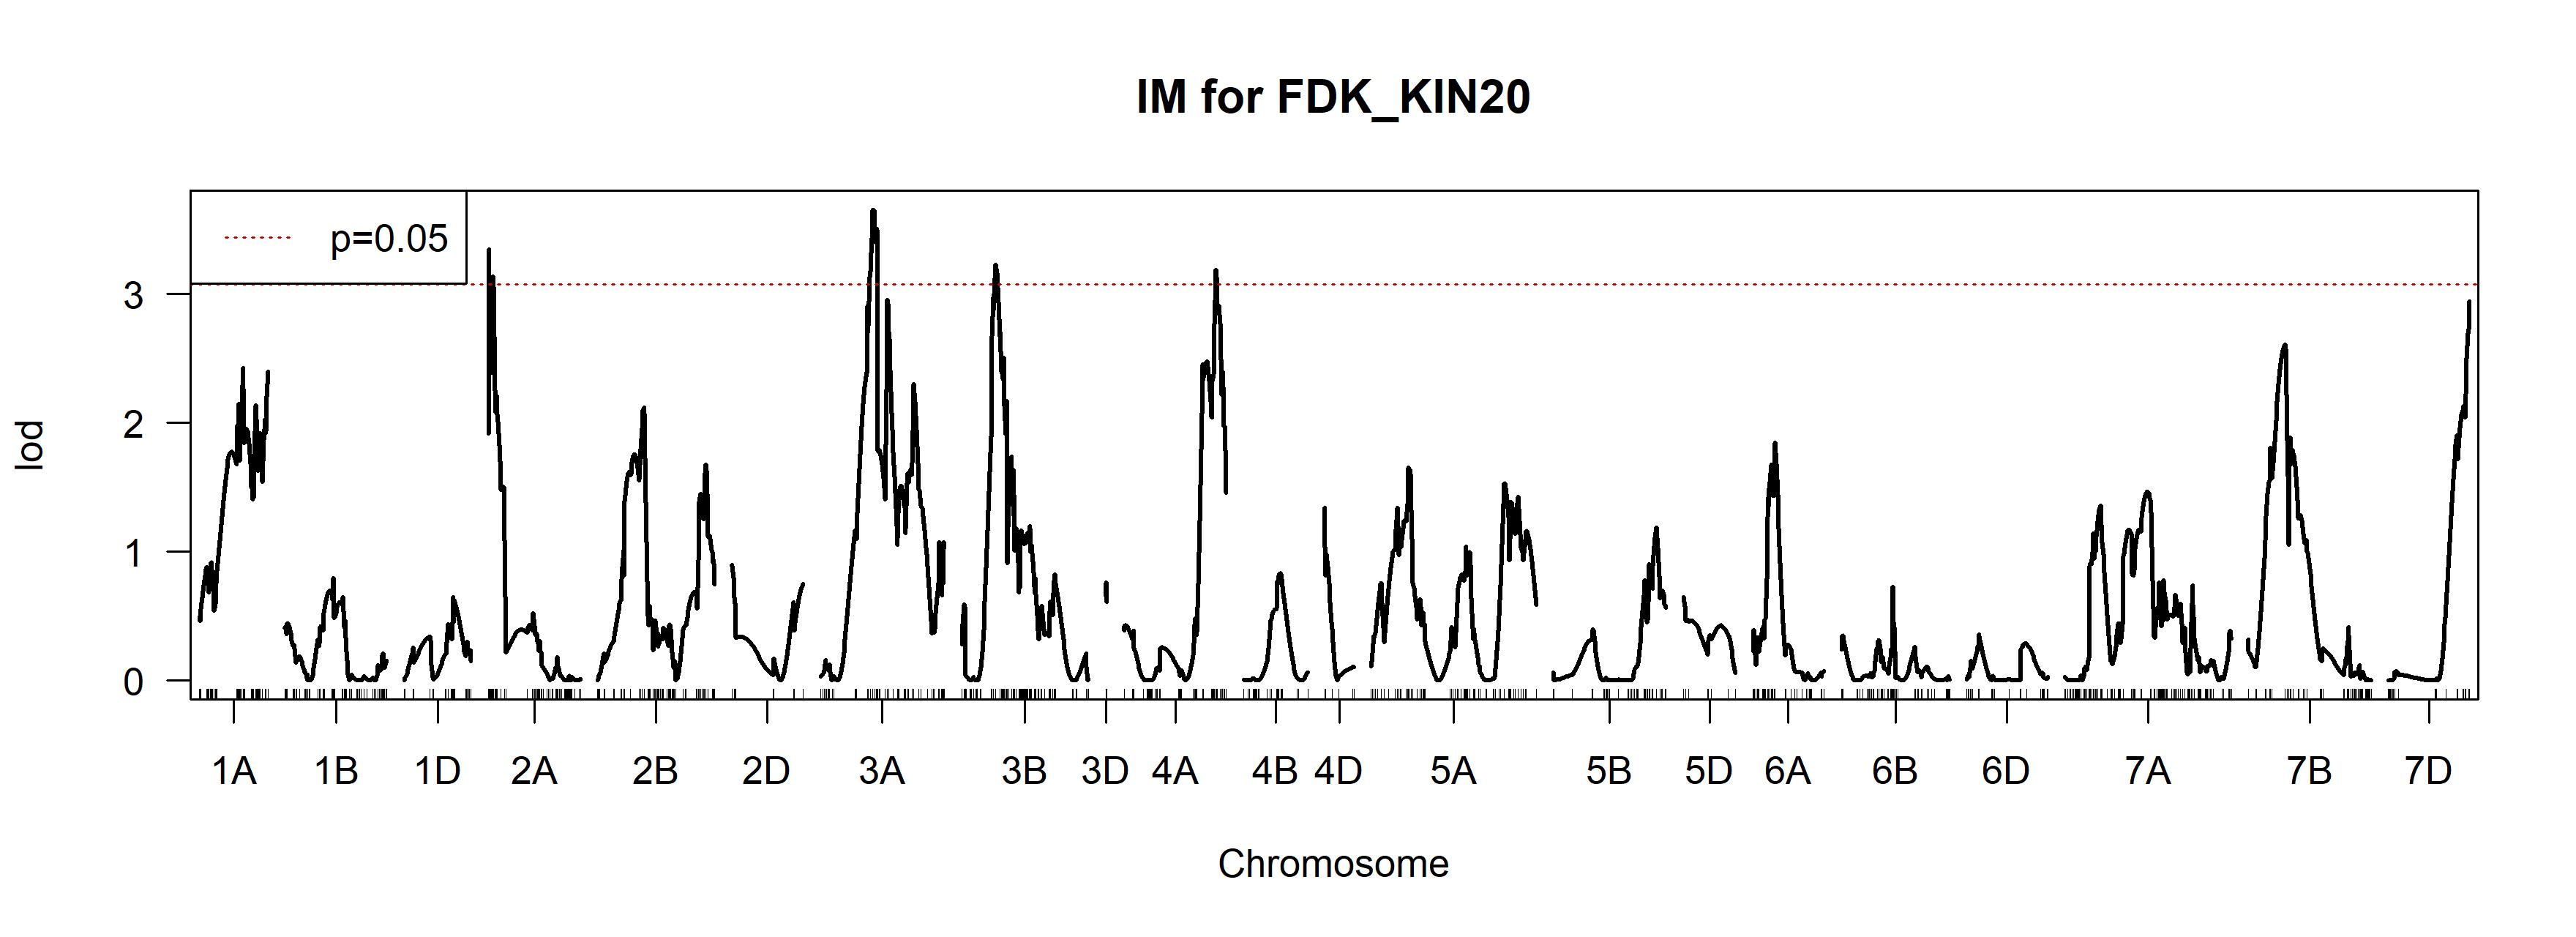
\includegraphics{Scan_IM_FDK_KIN20.jpg}
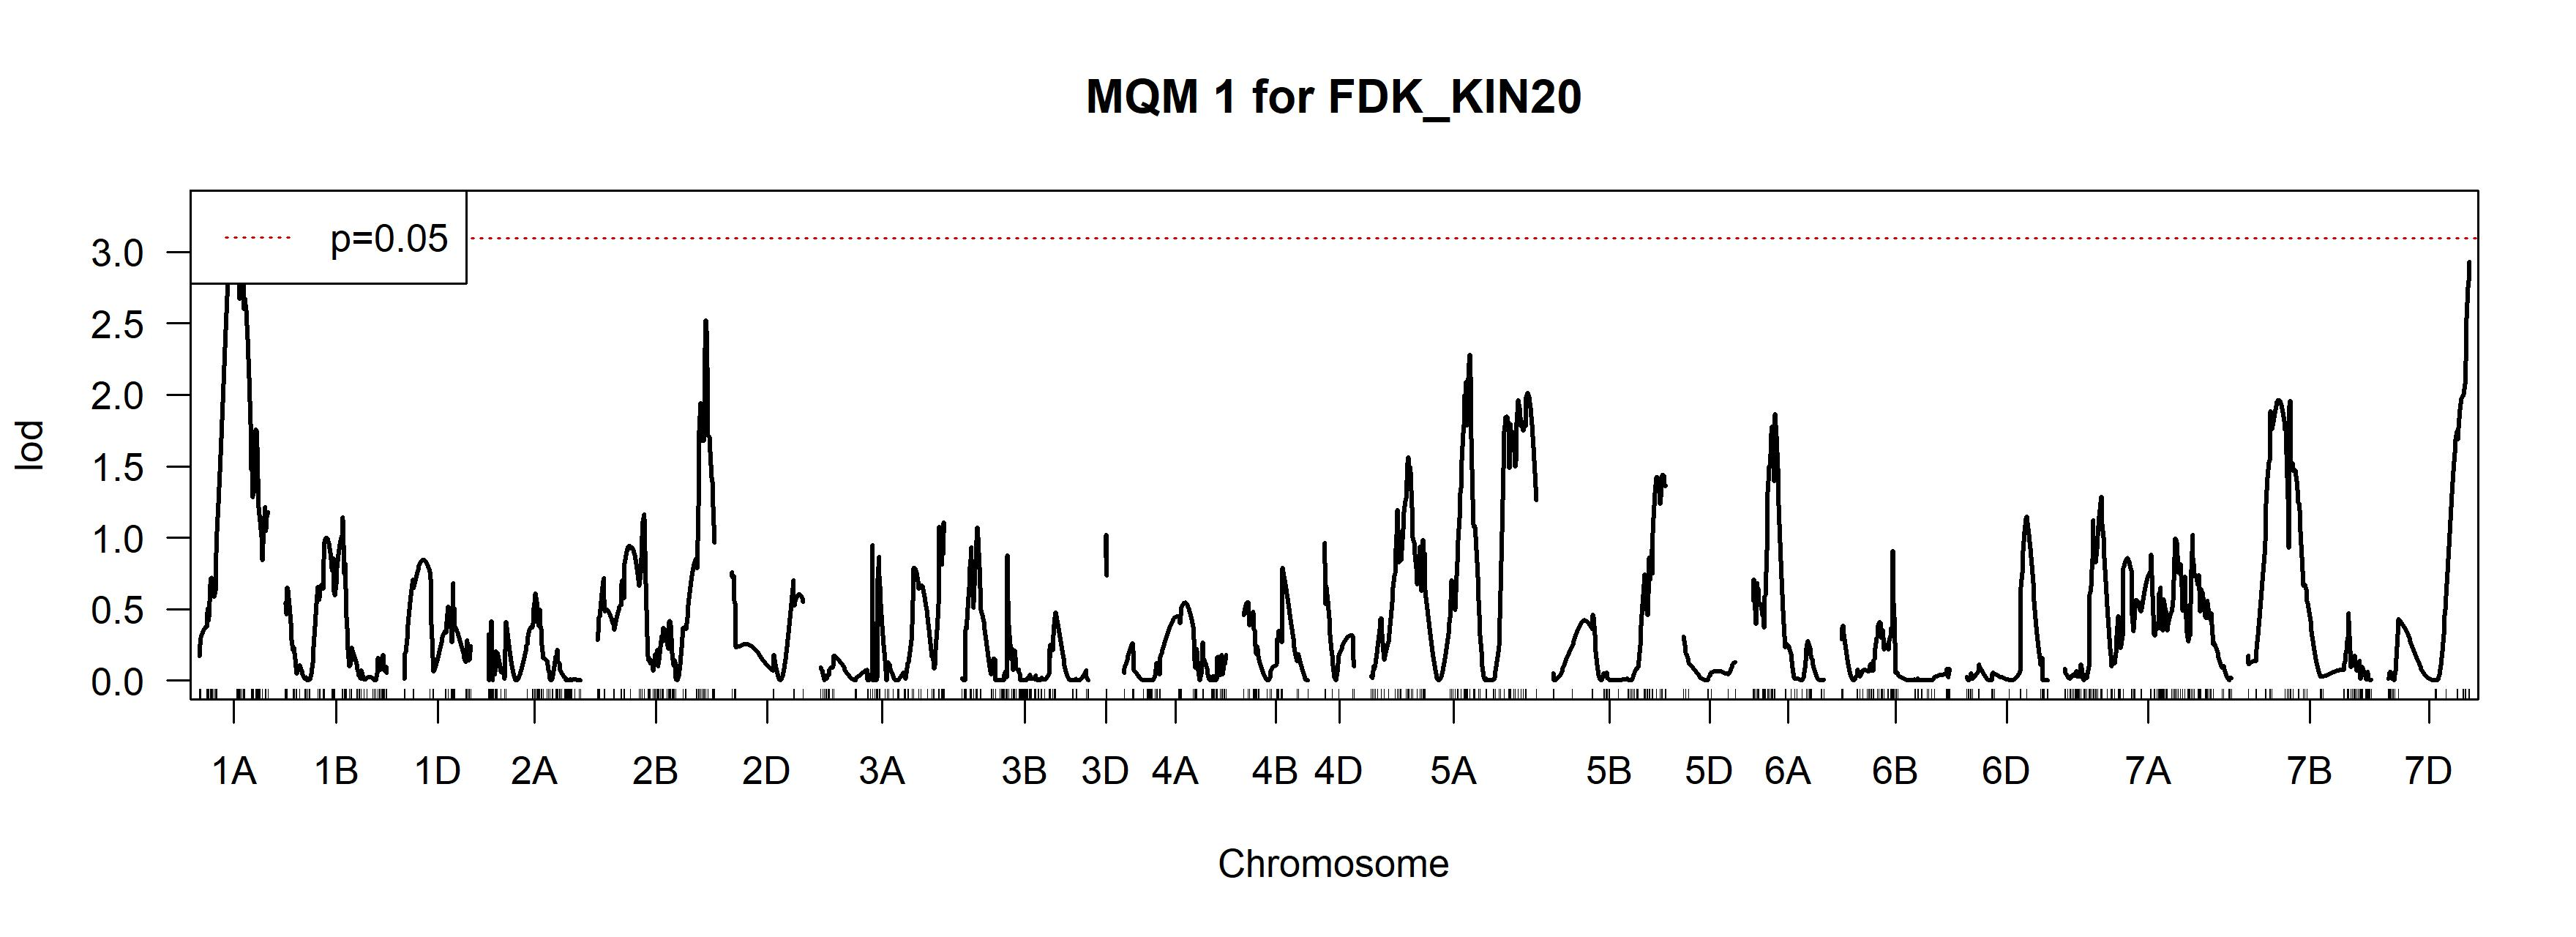
\includegraphics{Scan_MQM1_FDK_KIN20.jpg}
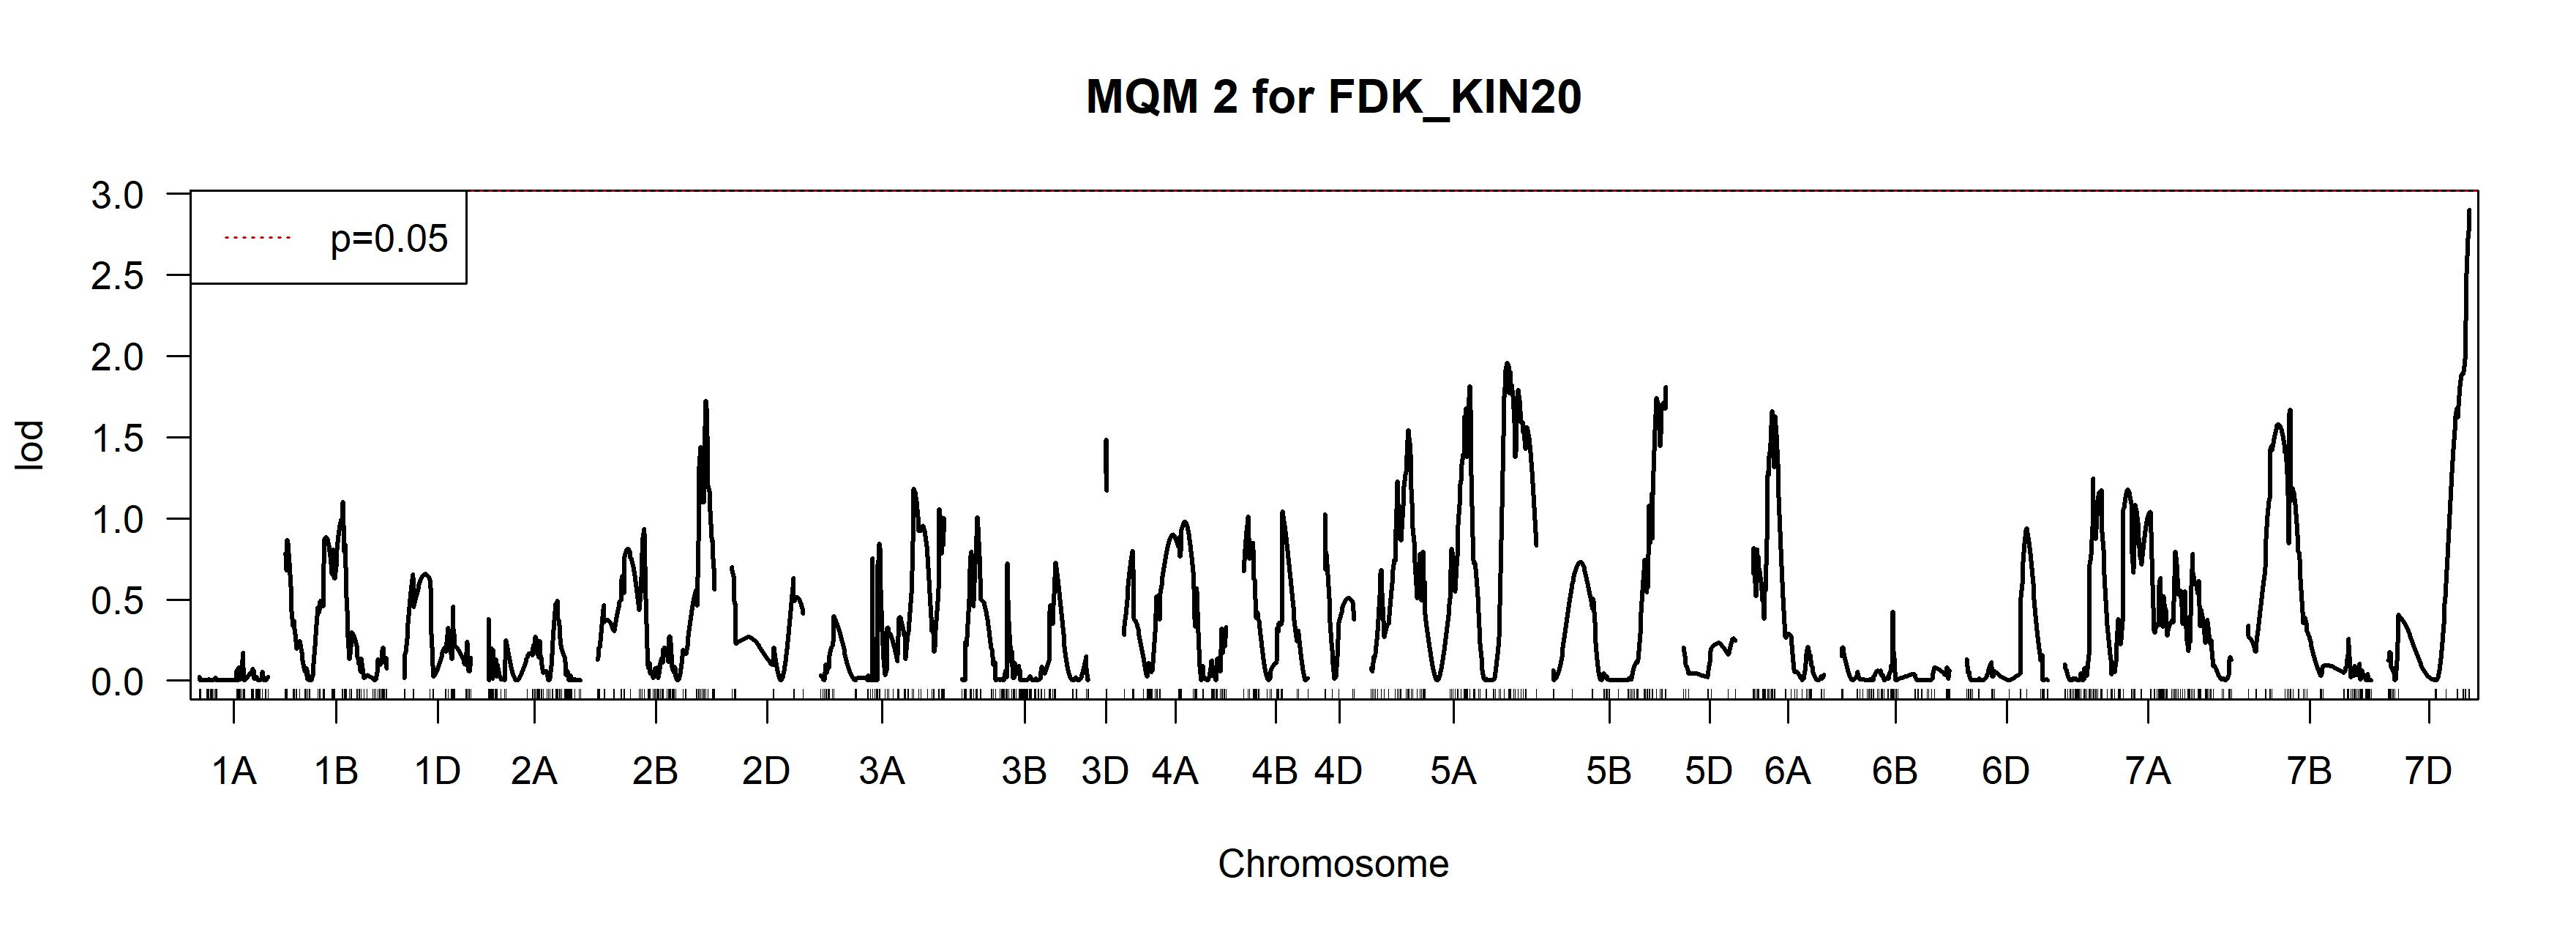
\includegraphics{Scan_MQM2_FDK_KIN20.jpg} \pagebreak

\subsection{Fusarium Damaged Kernels in Raleigh, NC -
2019}\label{fusarium-damaged-kernels-in-raleigh-nc---2019}

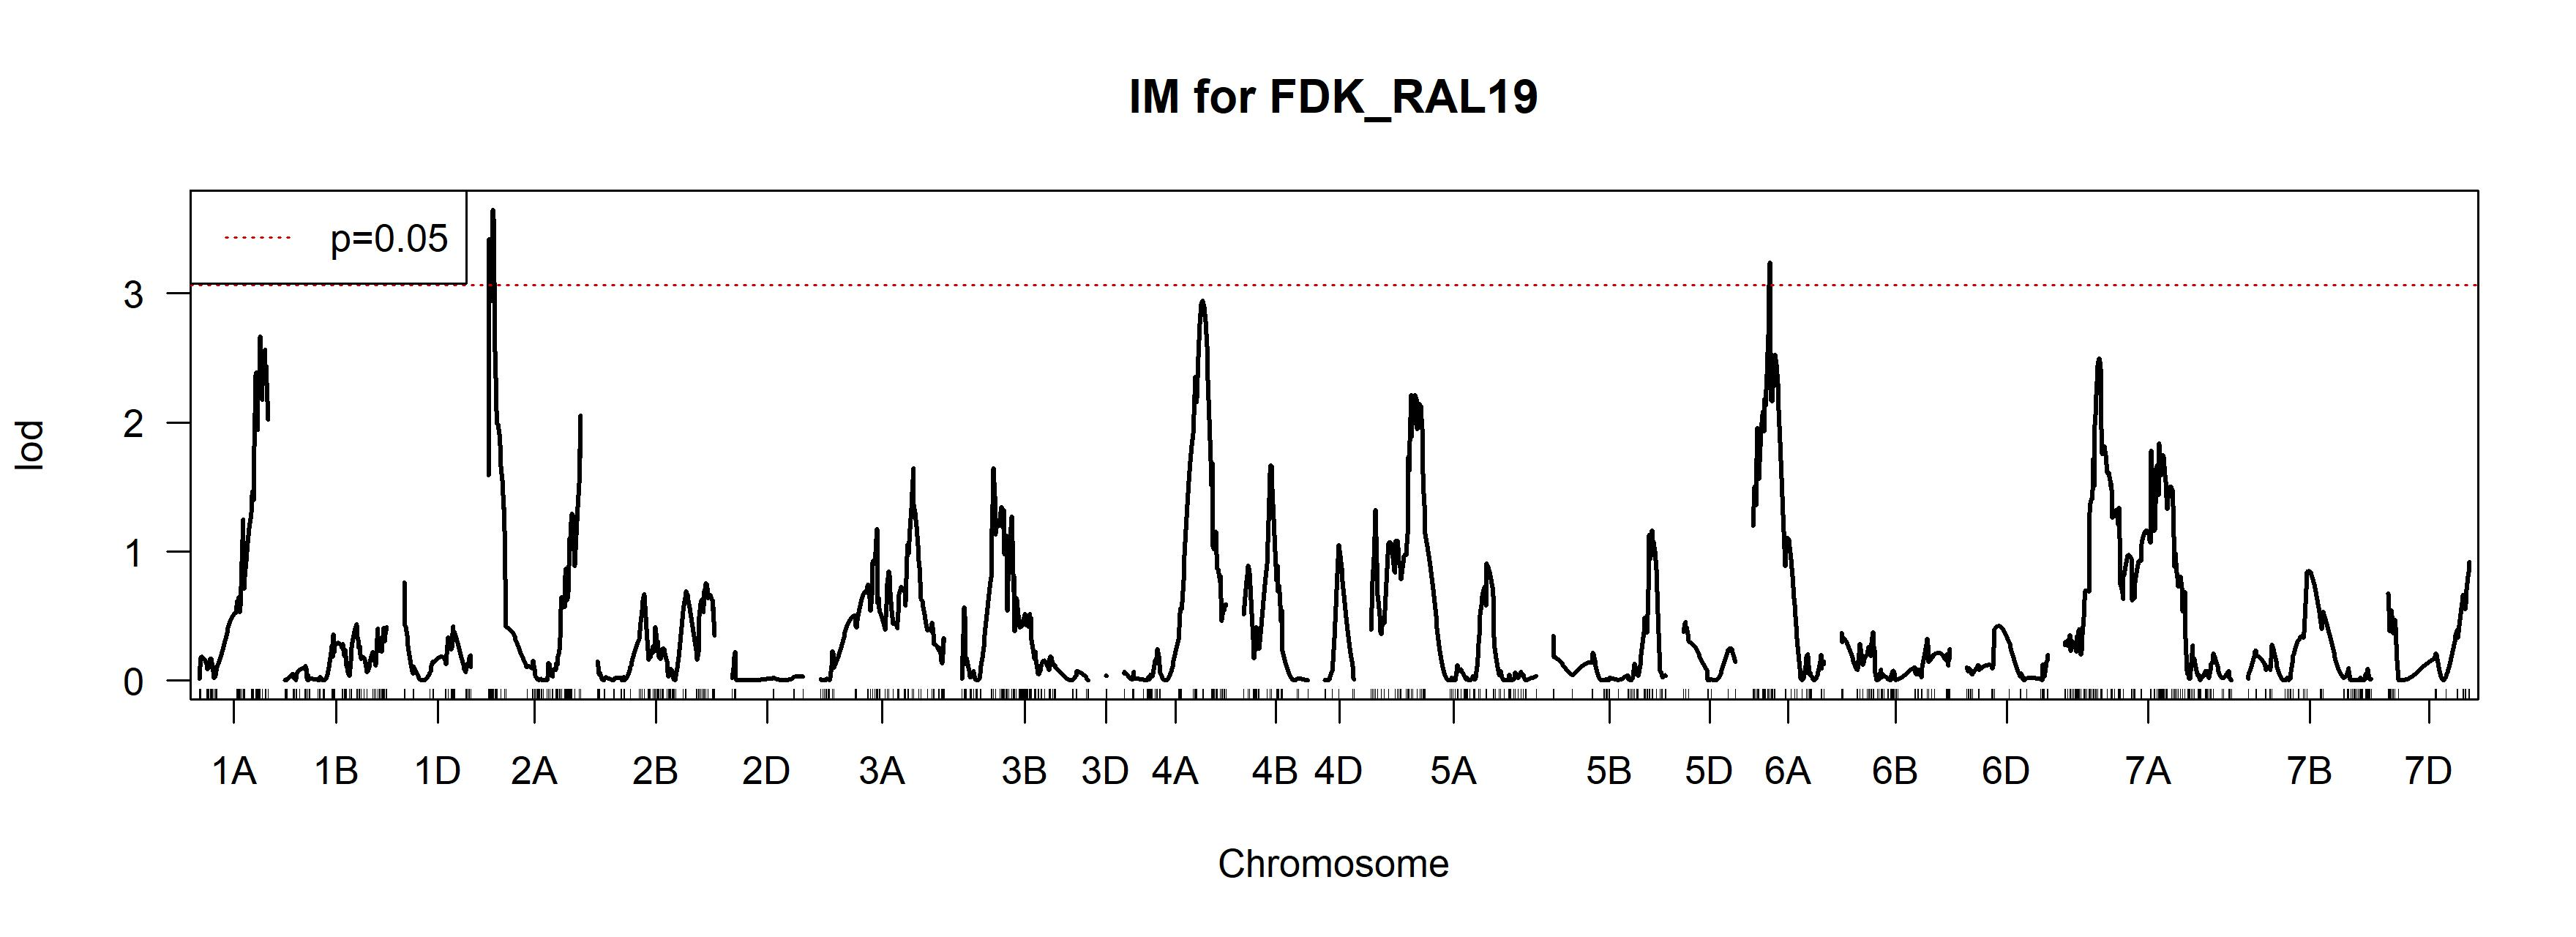
\includegraphics{Scan_IM_FDK_RAL19.jpg}
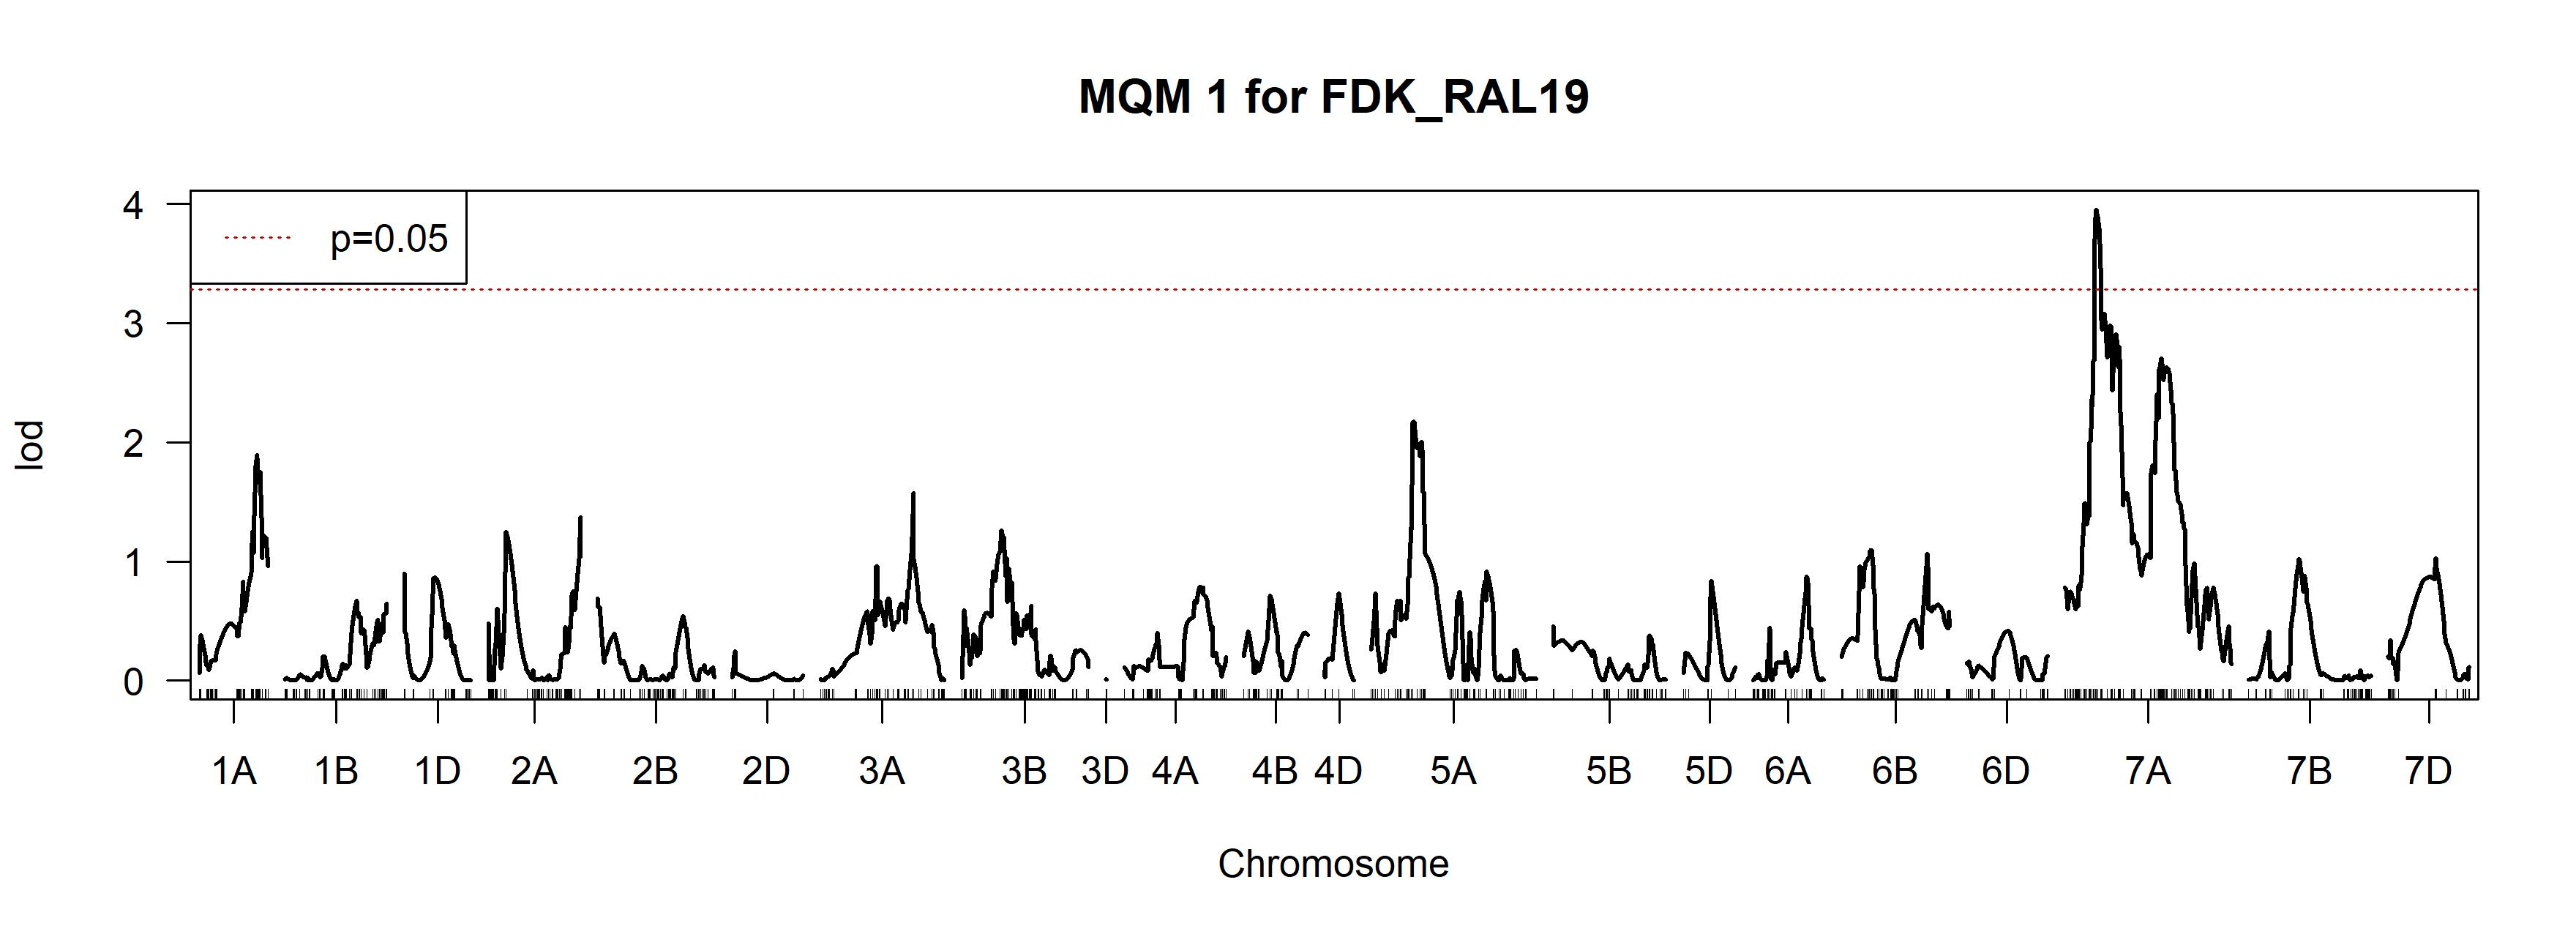
\includegraphics{Scan_MQM1_FDK_RAL19.jpg}
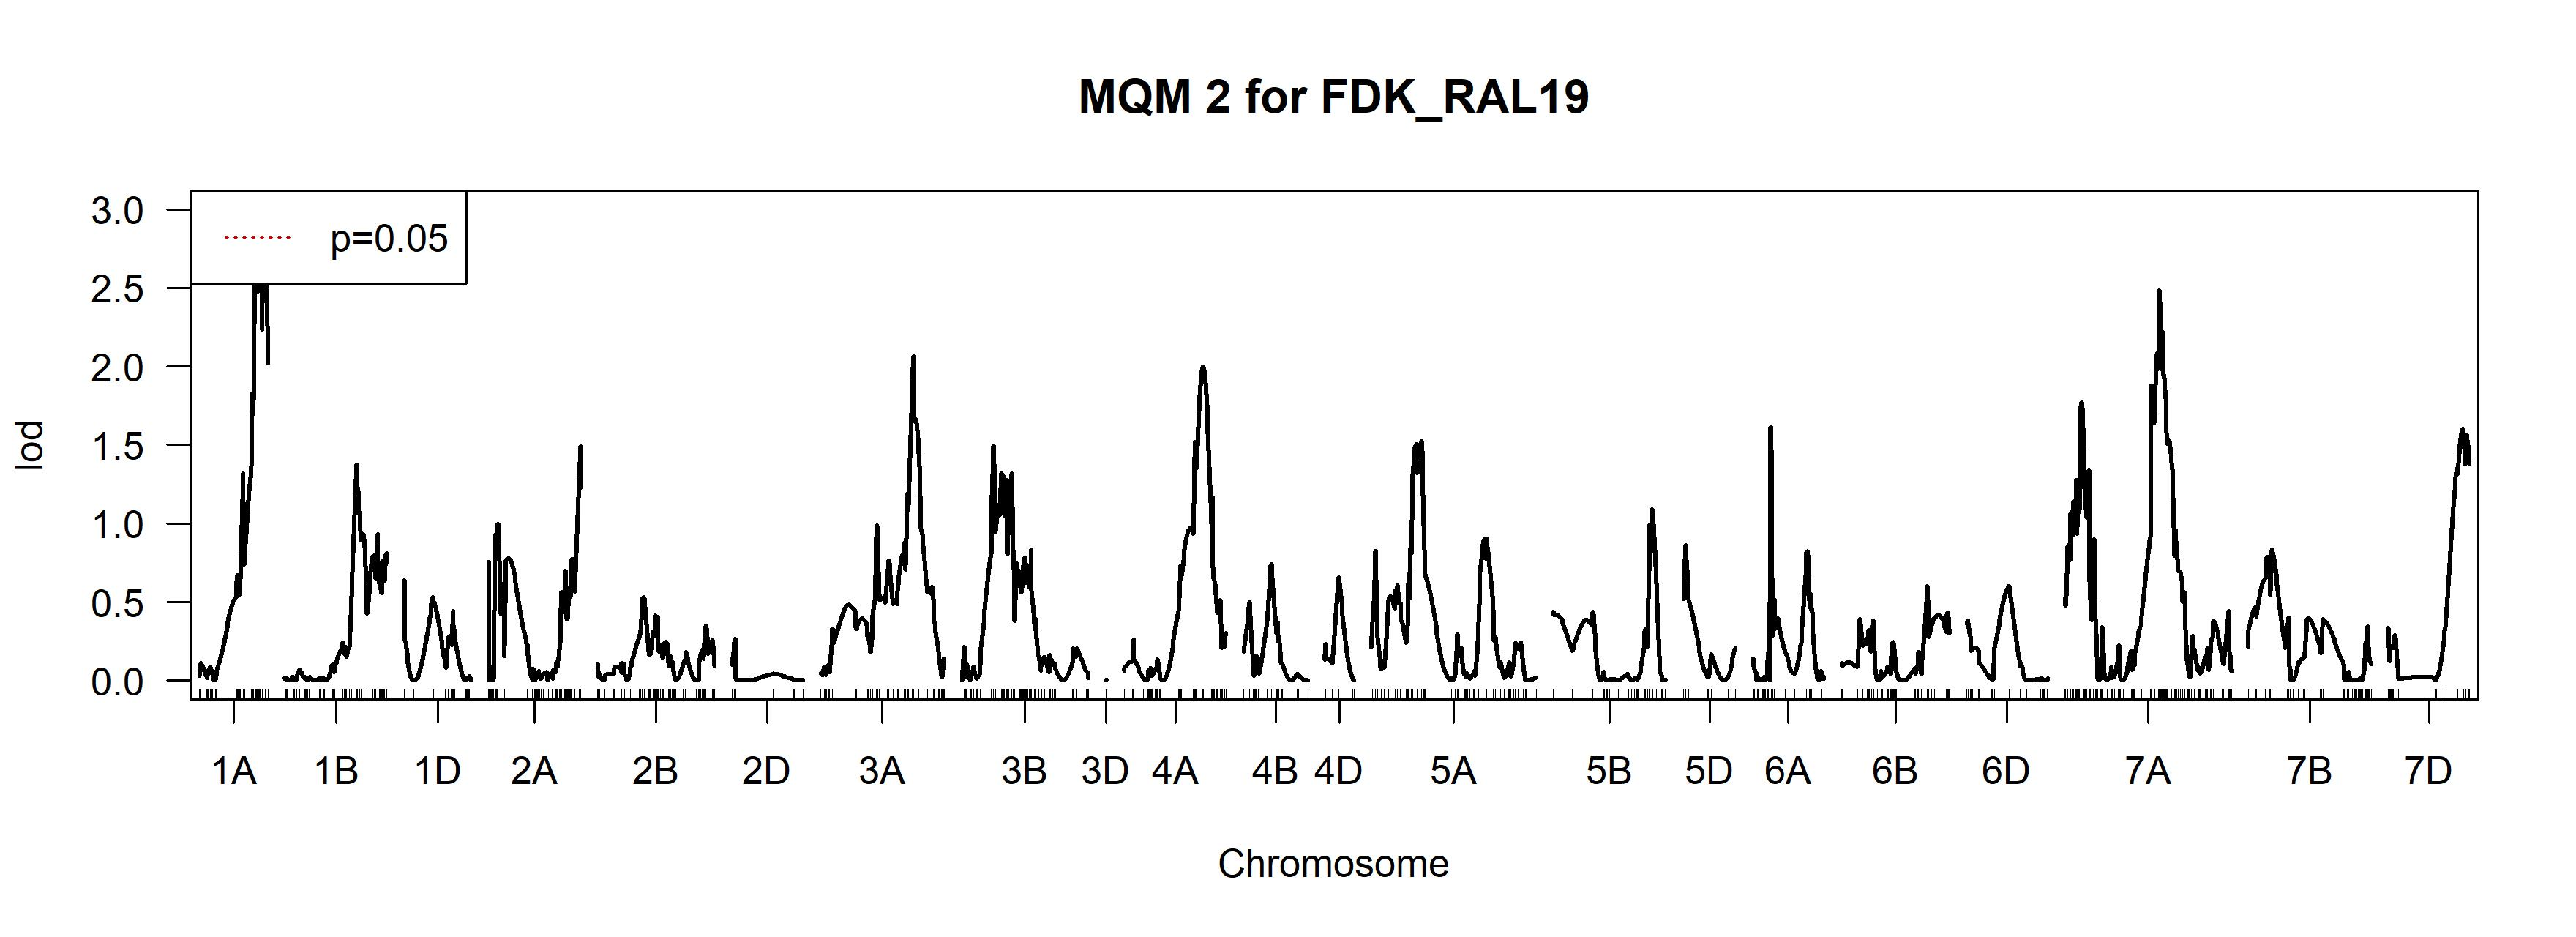
\includegraphics{Scan_MQM2_FDK_RAL19.jpg}
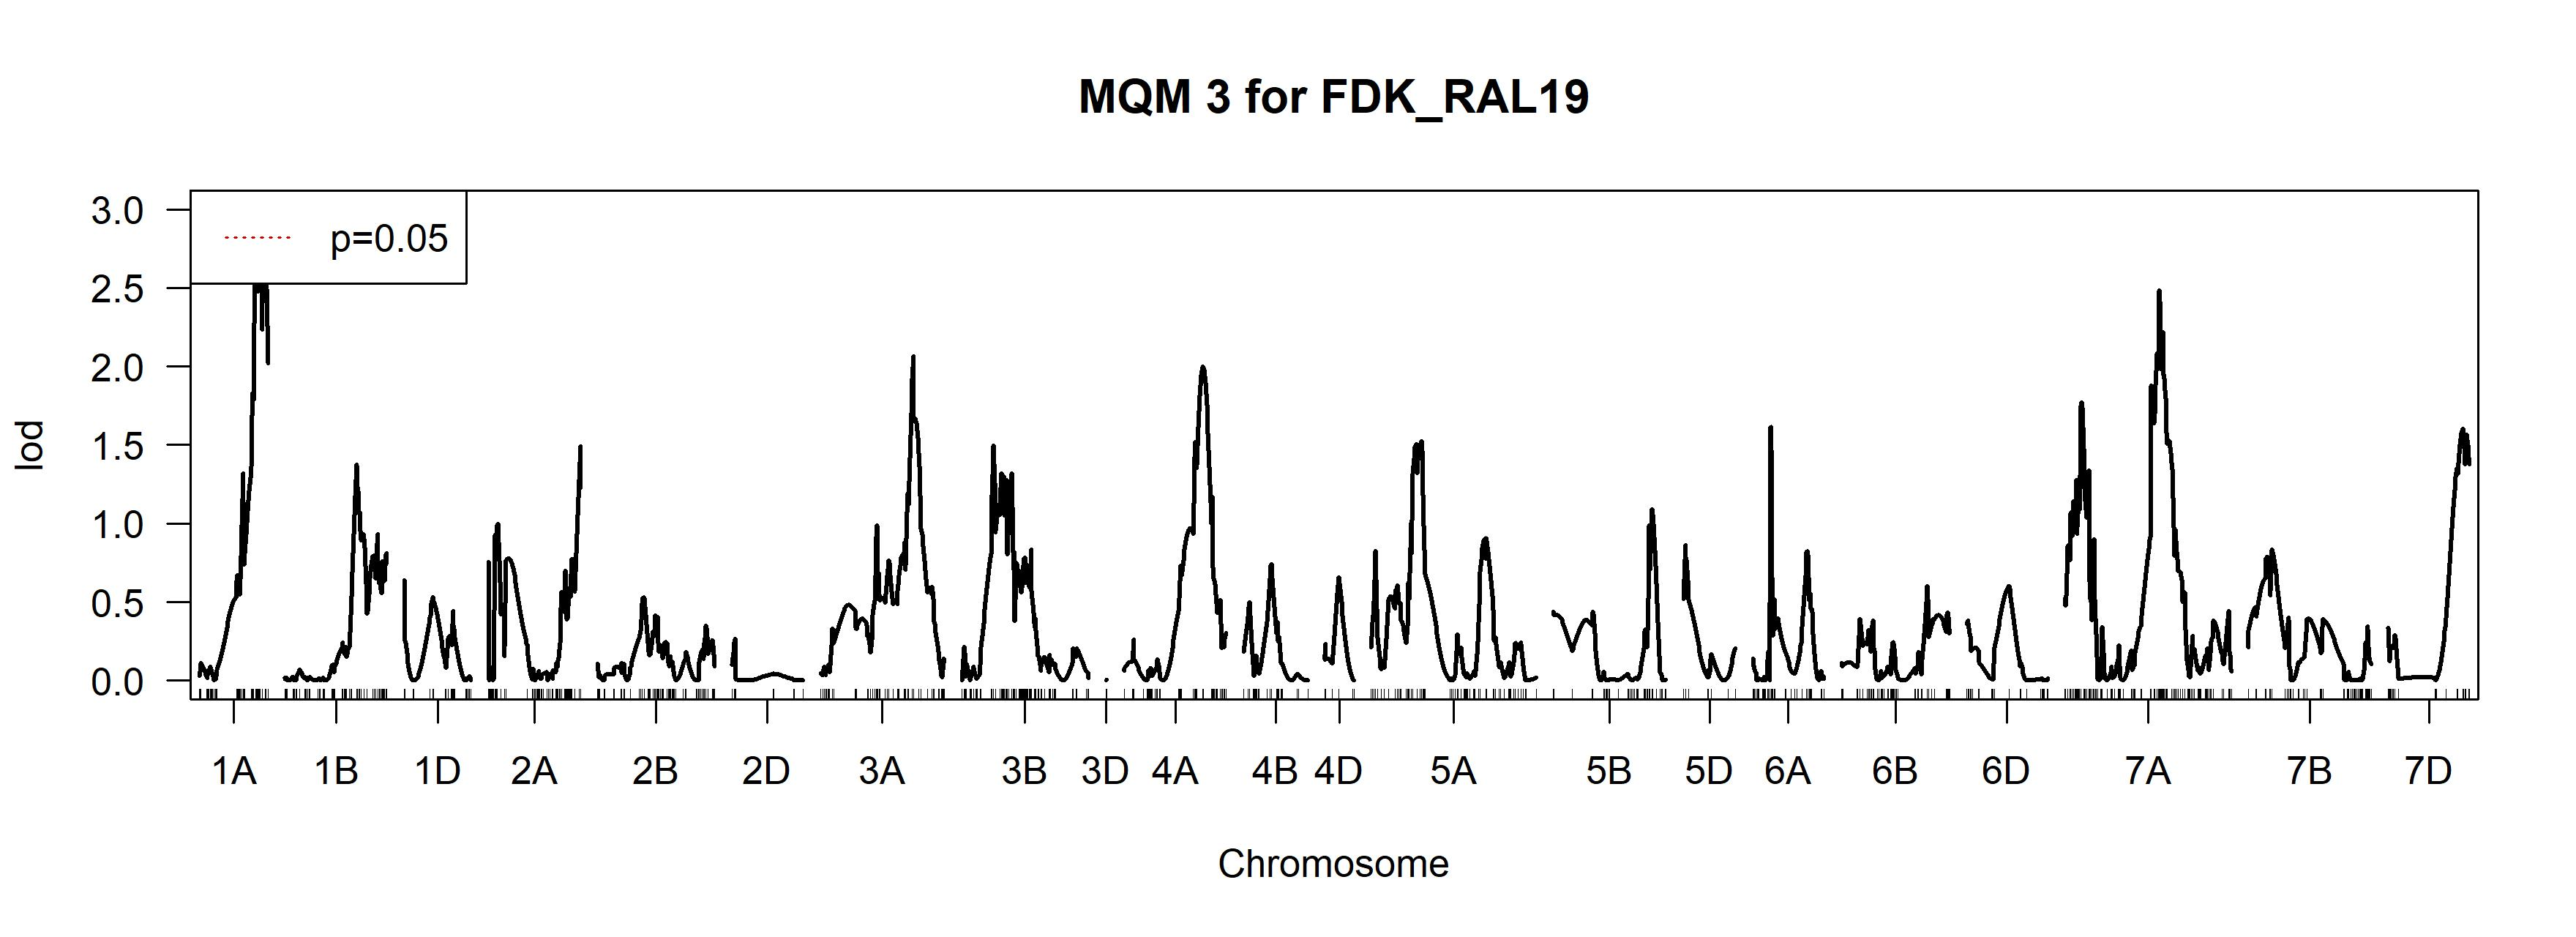
\includegraphics{Scan_MQM3_FDK_RAL19.jpg} \pagebreak

\subsection{Fusarium Damaged Kernels in Raleigh, NC -
2020}\label{fusarium-damaged-kernels-in-raleigh-nc---2020}

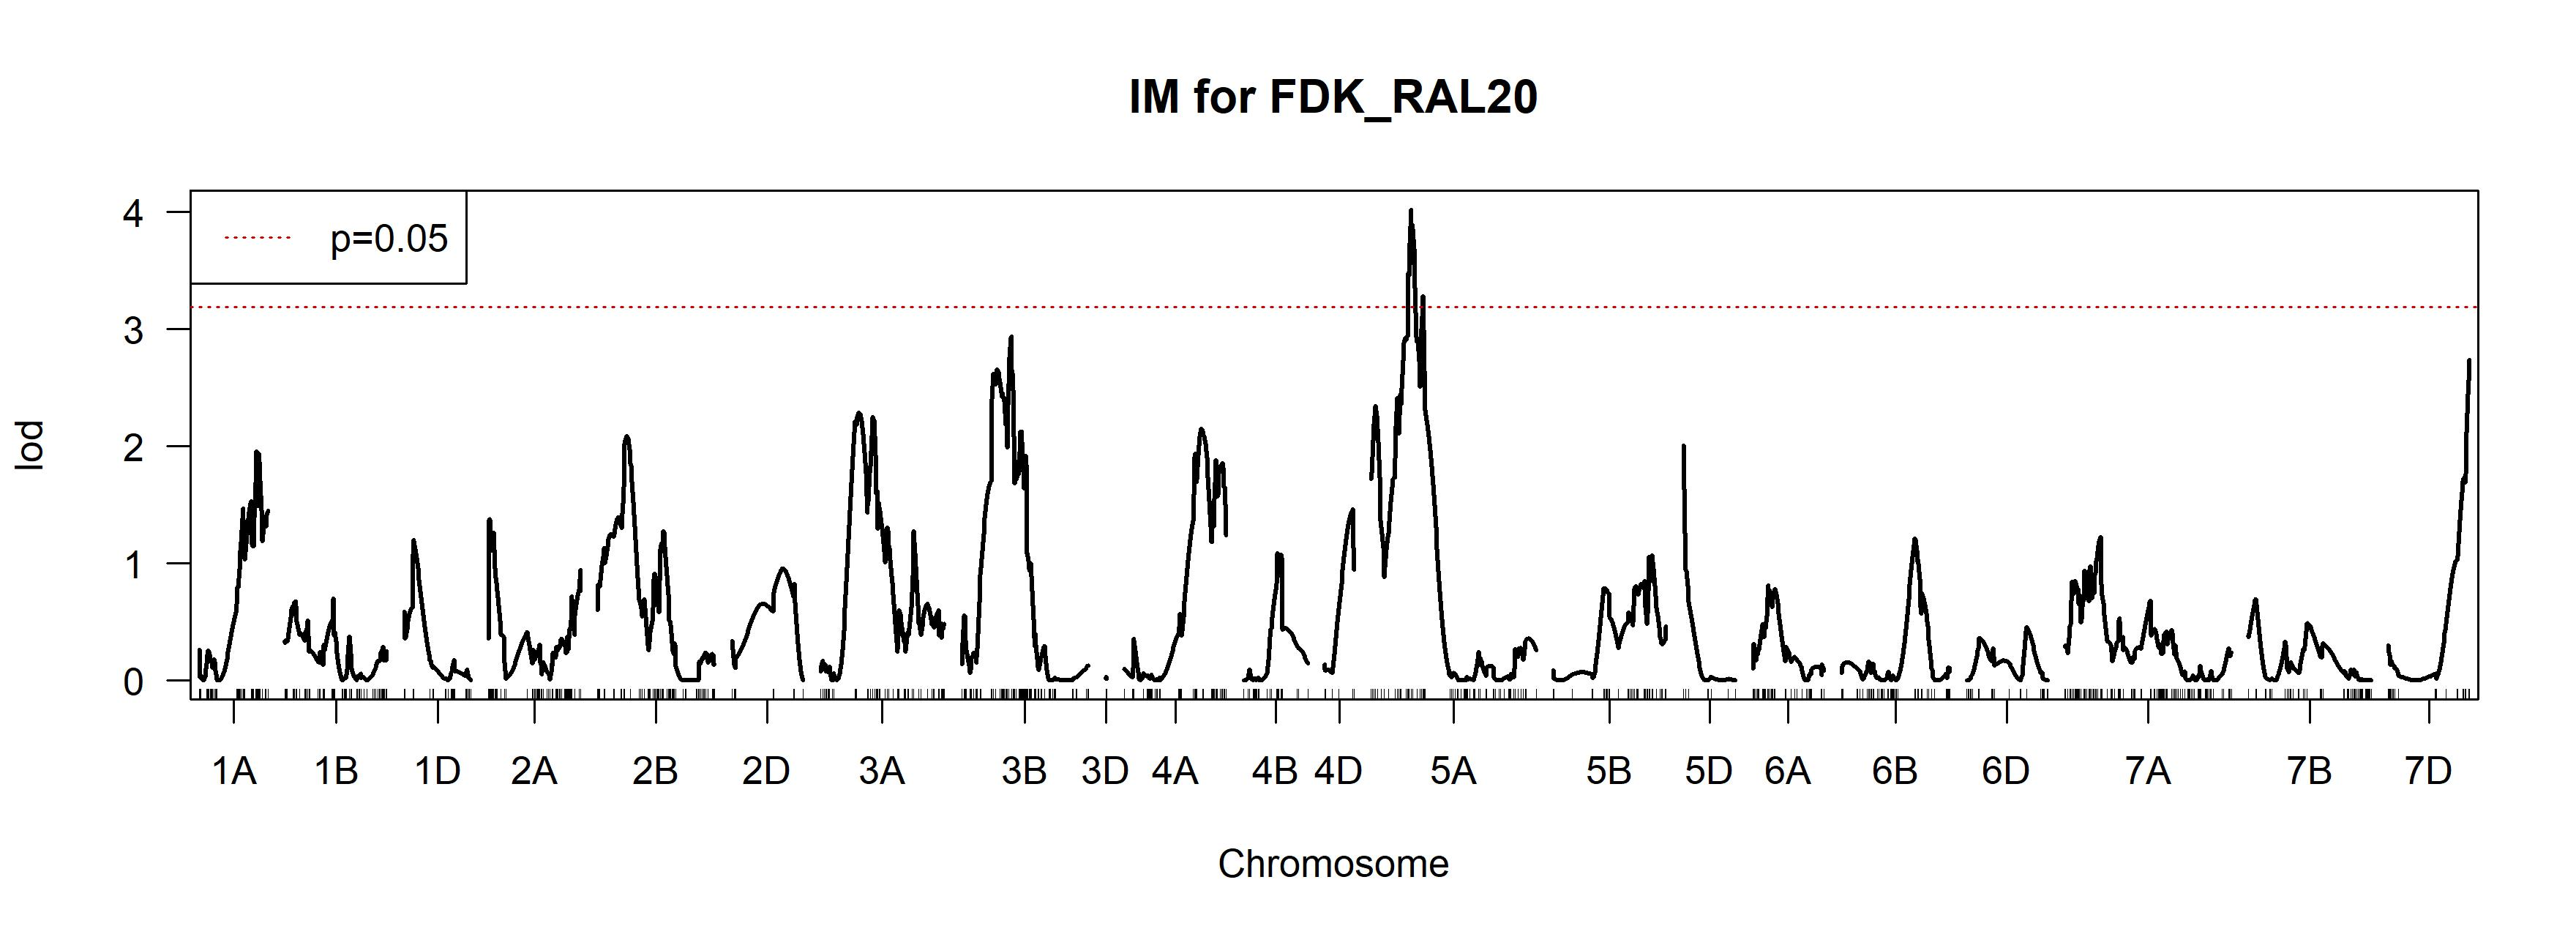
\includegraphics{Scan_IM_FDK_RAL20.jpg}
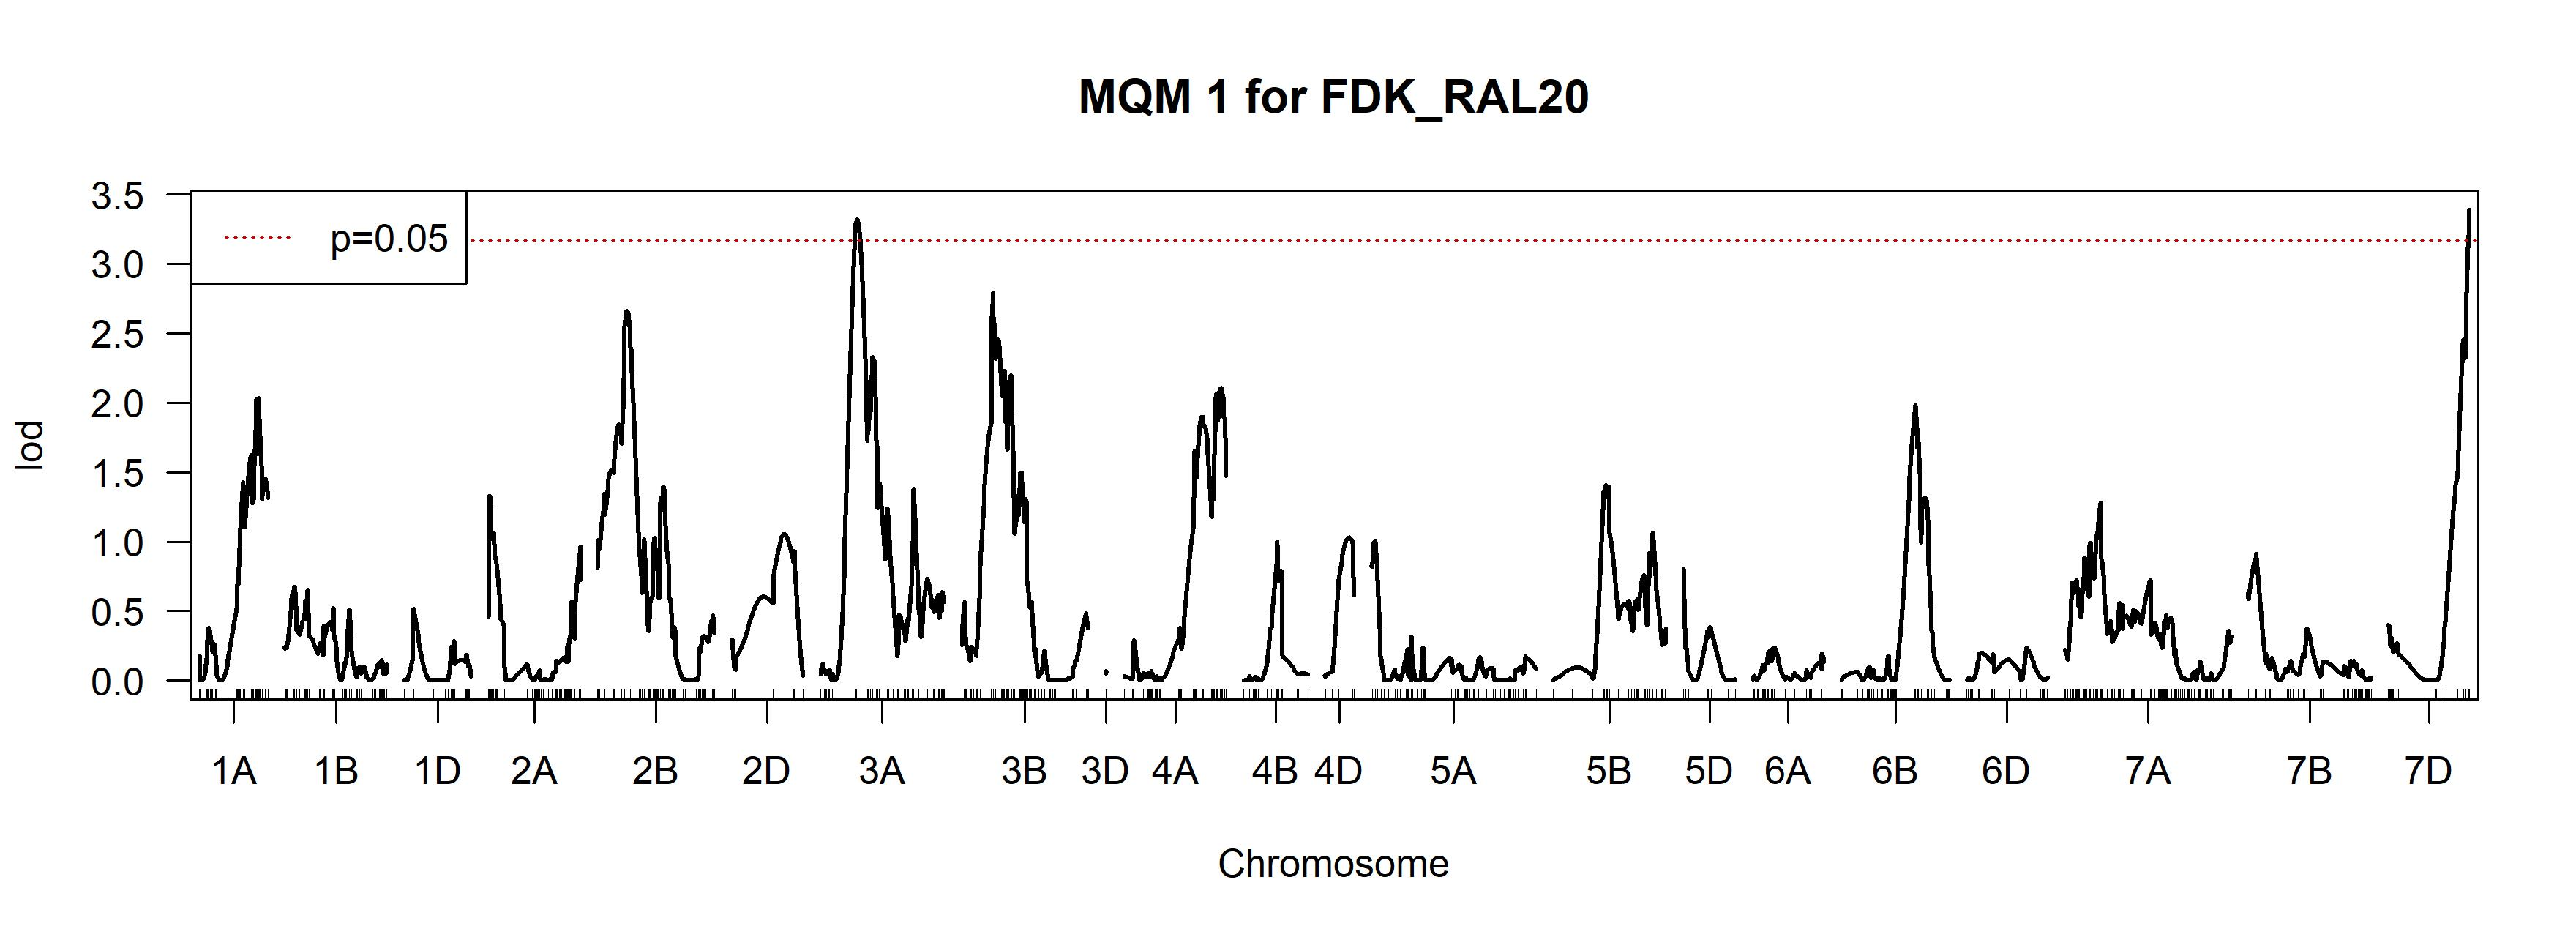
\includegraphics{Scan_MQM1_FDK_RAL20.jpg}
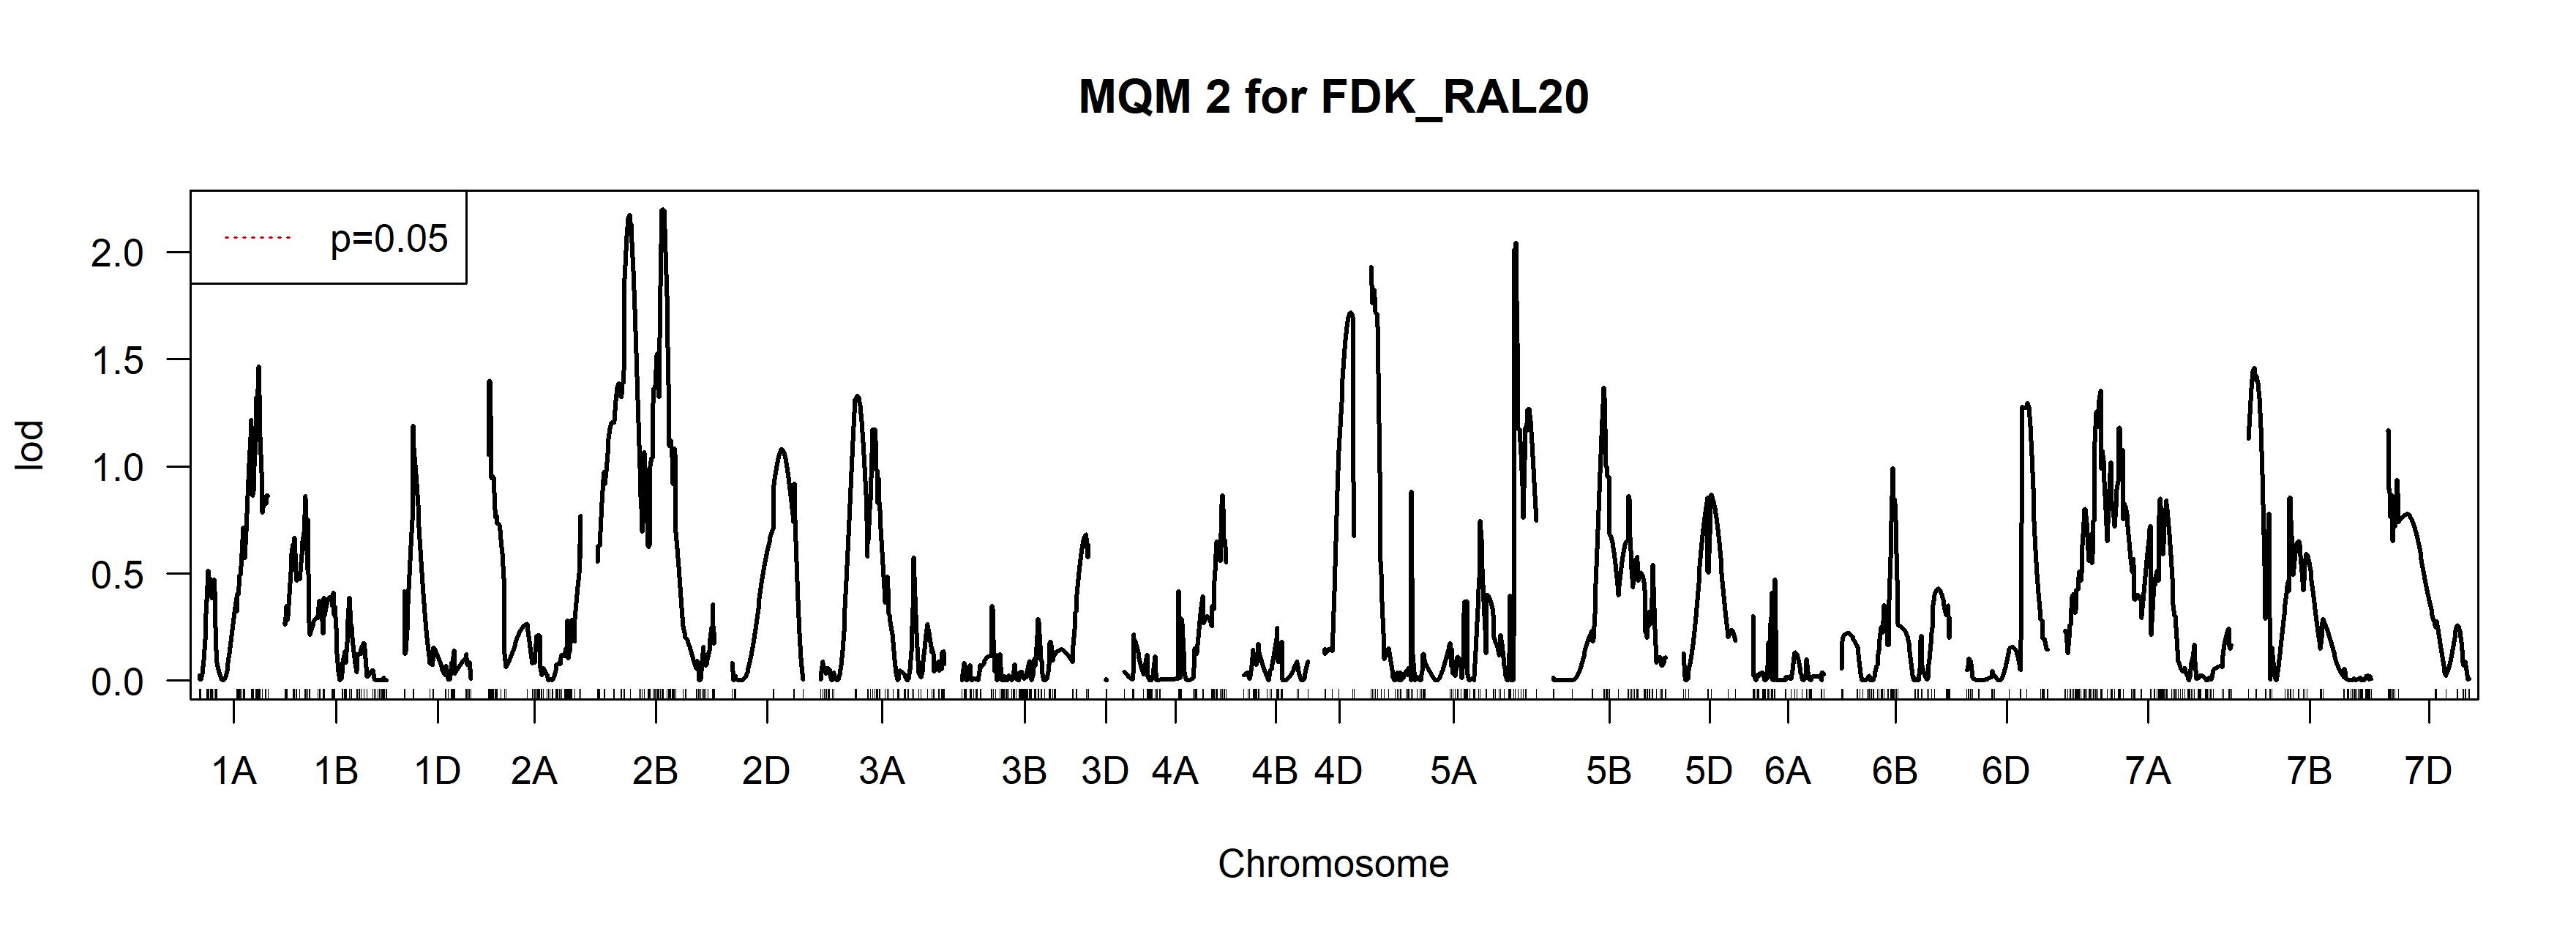
\includegraphics{Scan_MQM2_FDK_RAL20.jpg} \pagebreak

\subsection{Fusarium Damaged Kernels in Warsaw, VA -
2019}\label{fusarium-damaged-kernels-in-warsaw-va---2019}

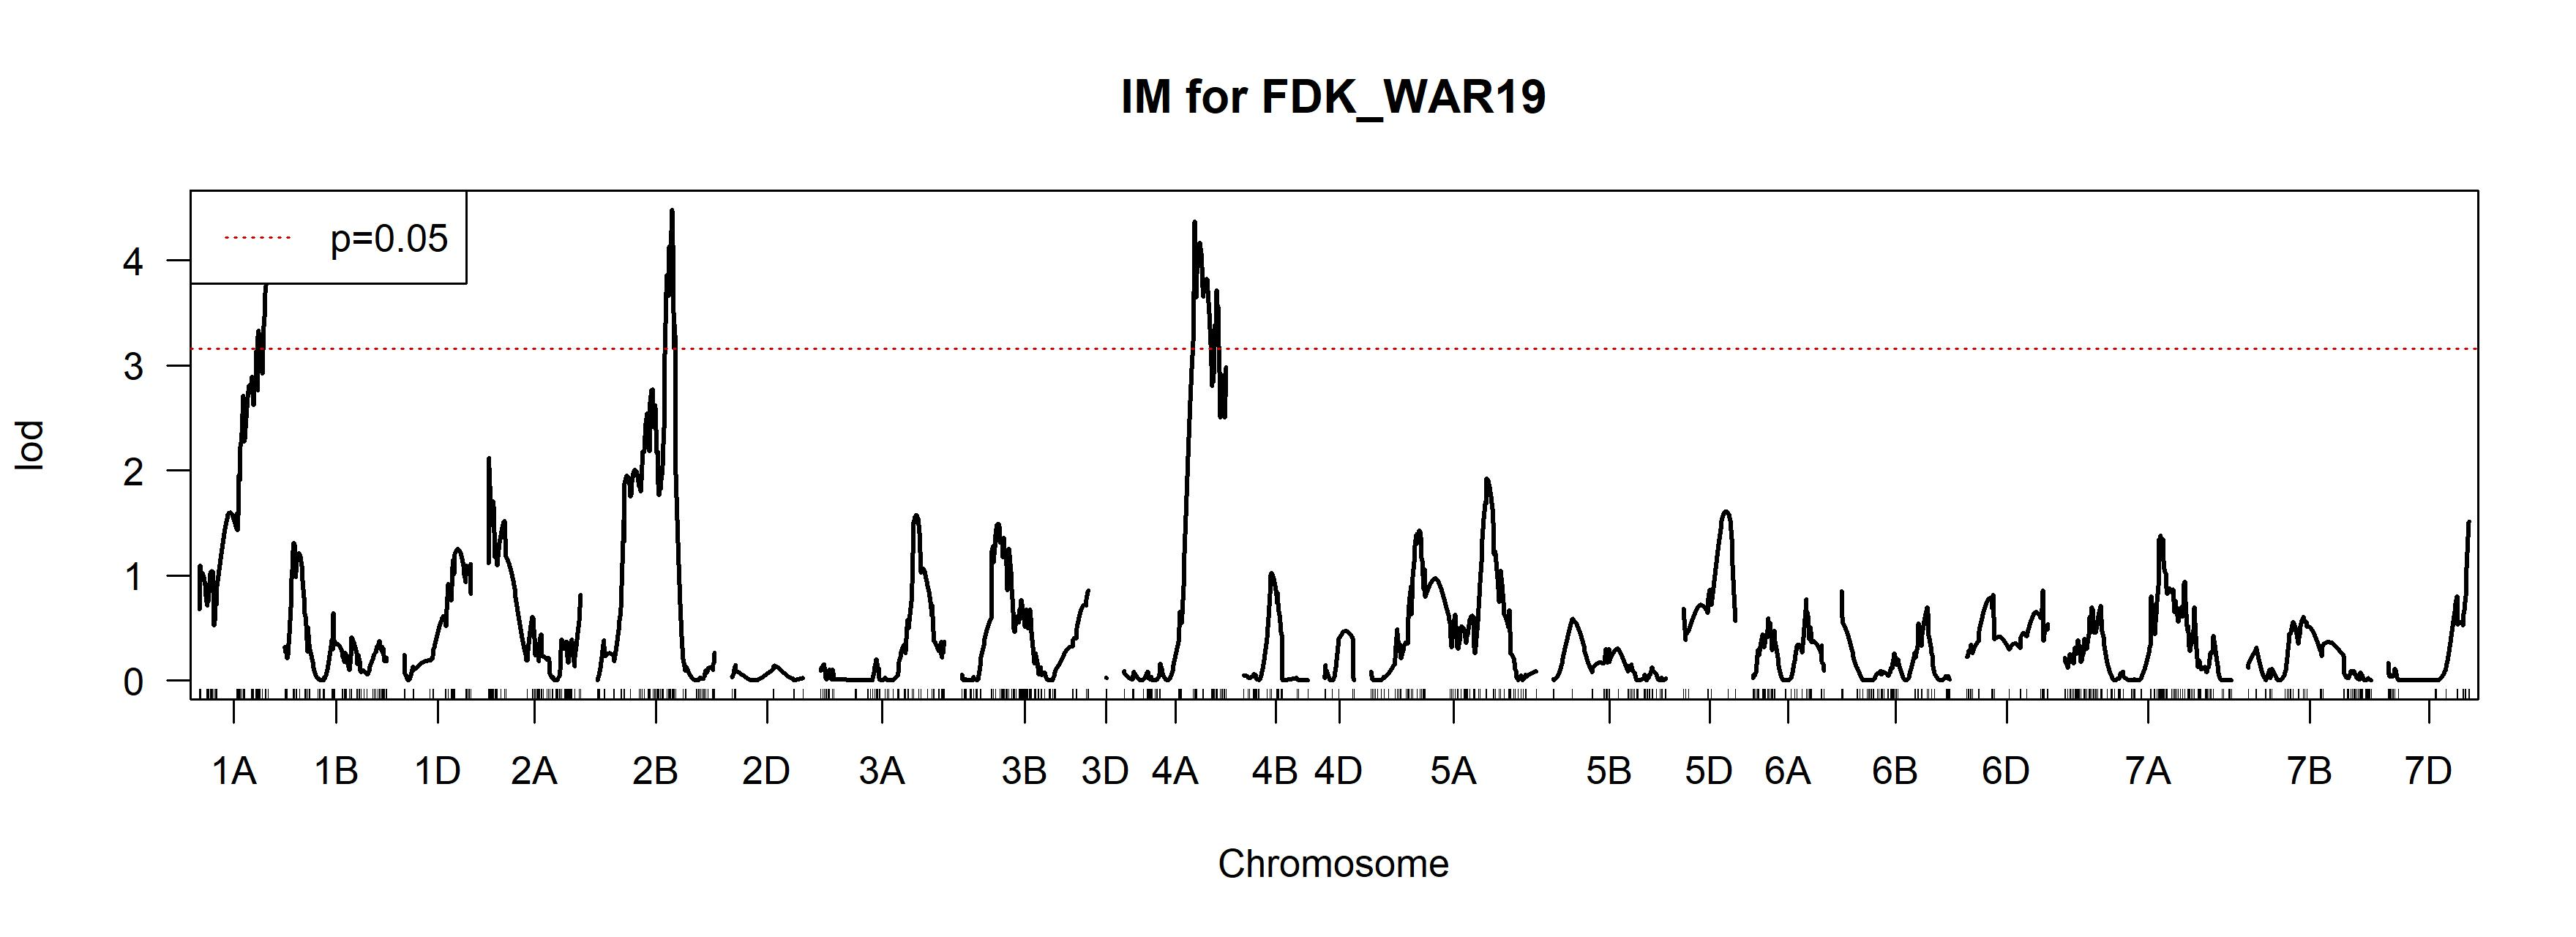
\includegraphics{Scan_IM_FDK_WAR19.jpg}
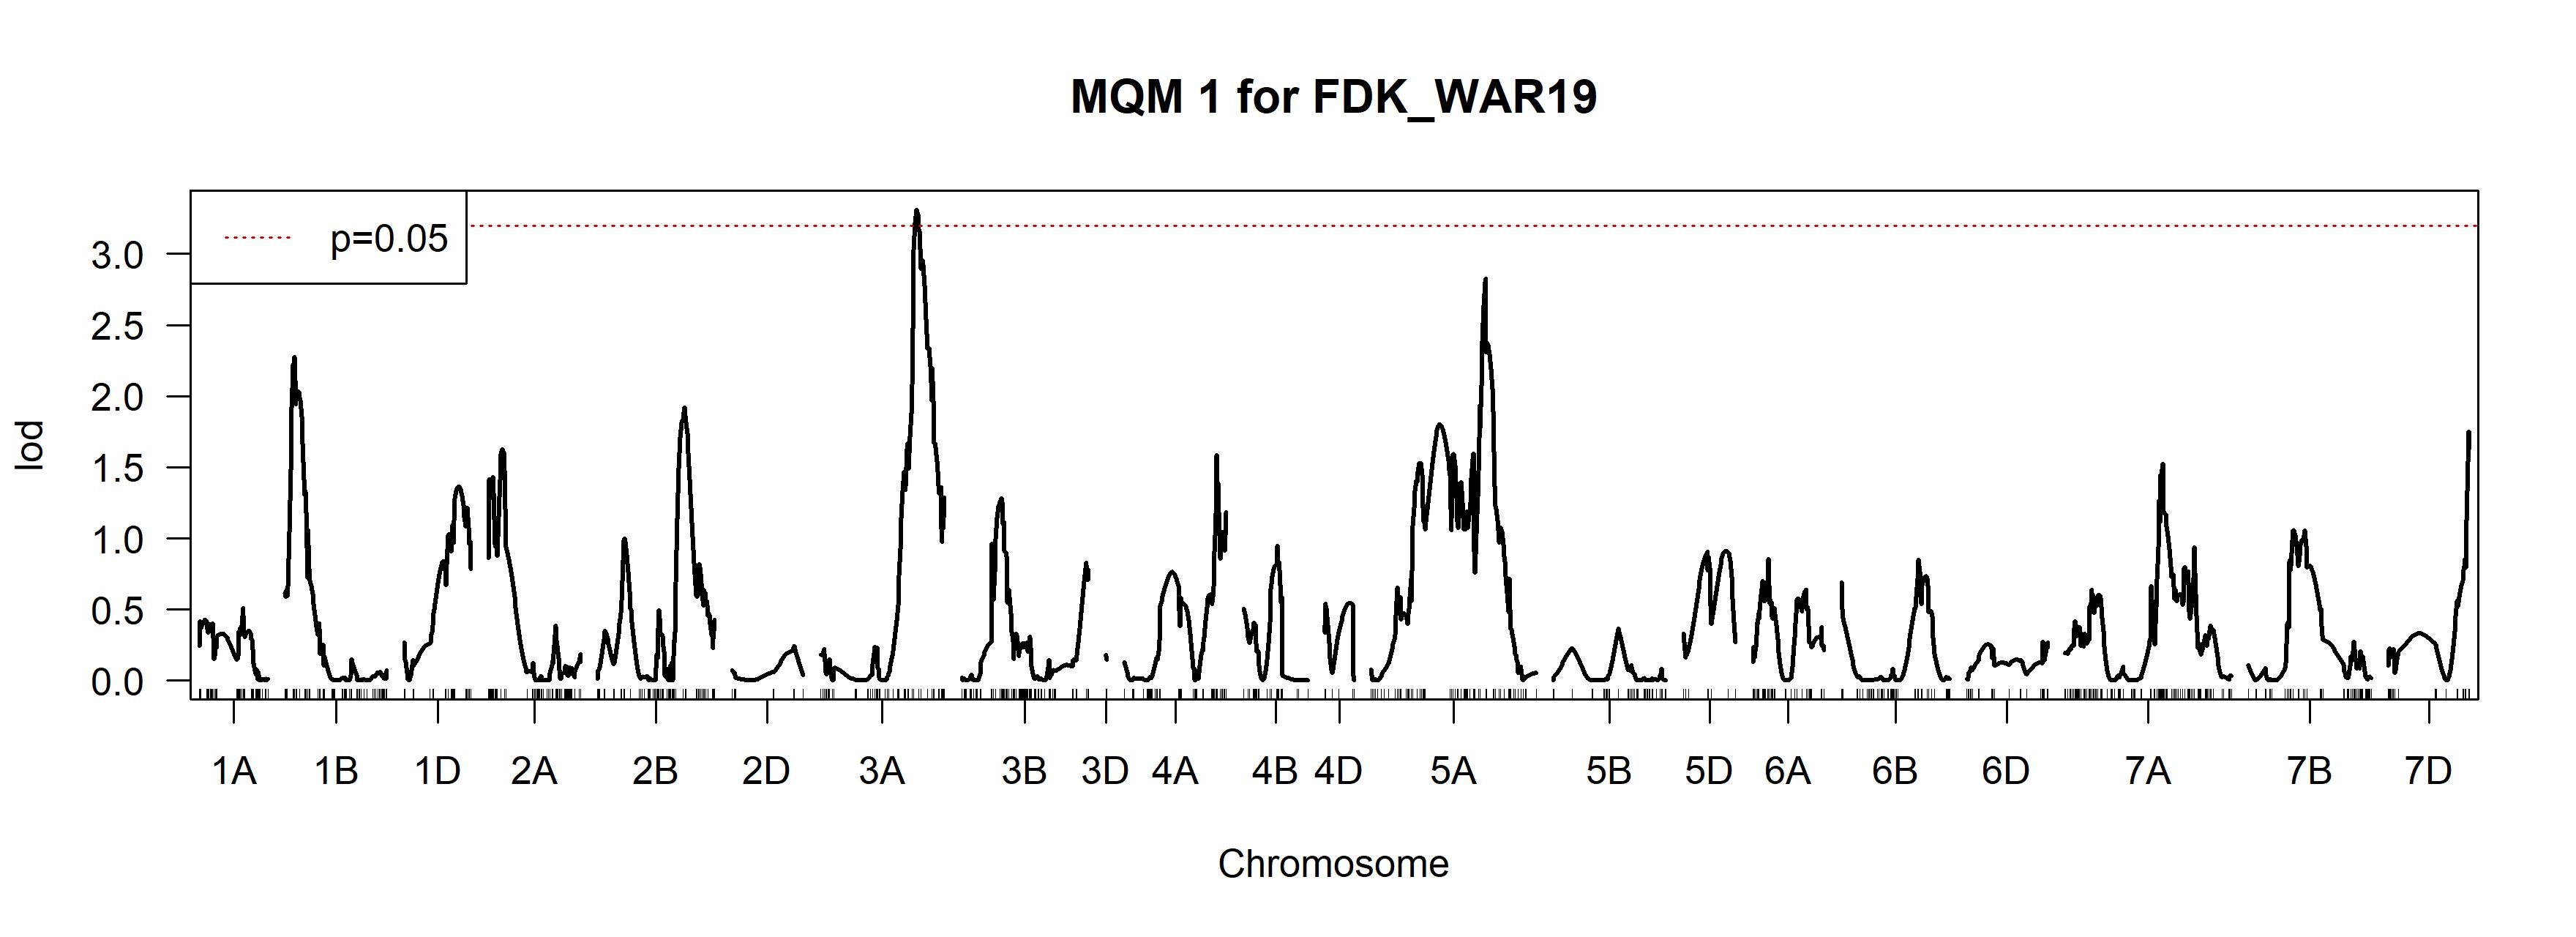
\includegraphics{Scan_MQM1_FDK_WAR19.jpg}
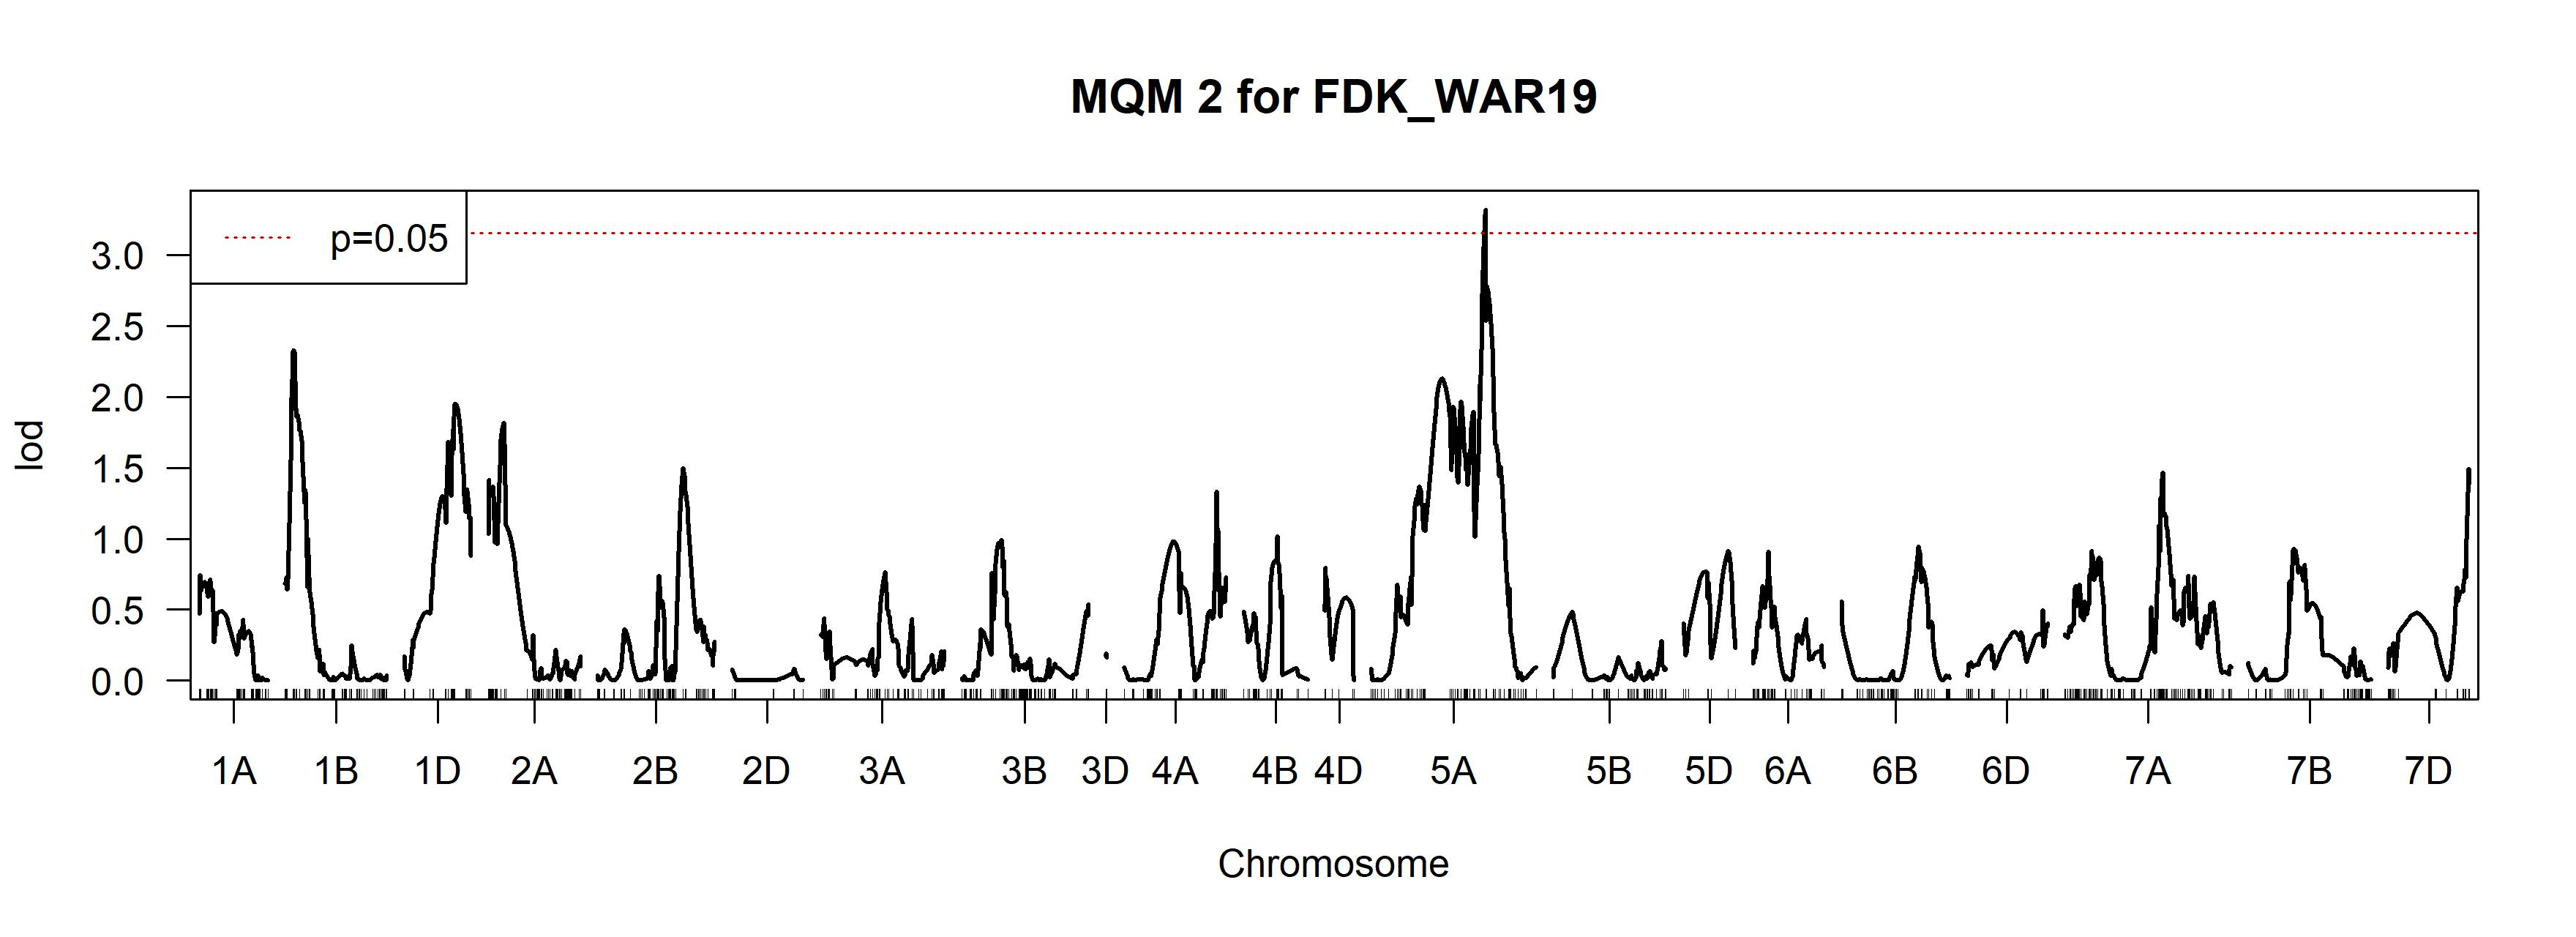
\includegraphics{Scan_MQM2_FDK_WAR19.jpg}
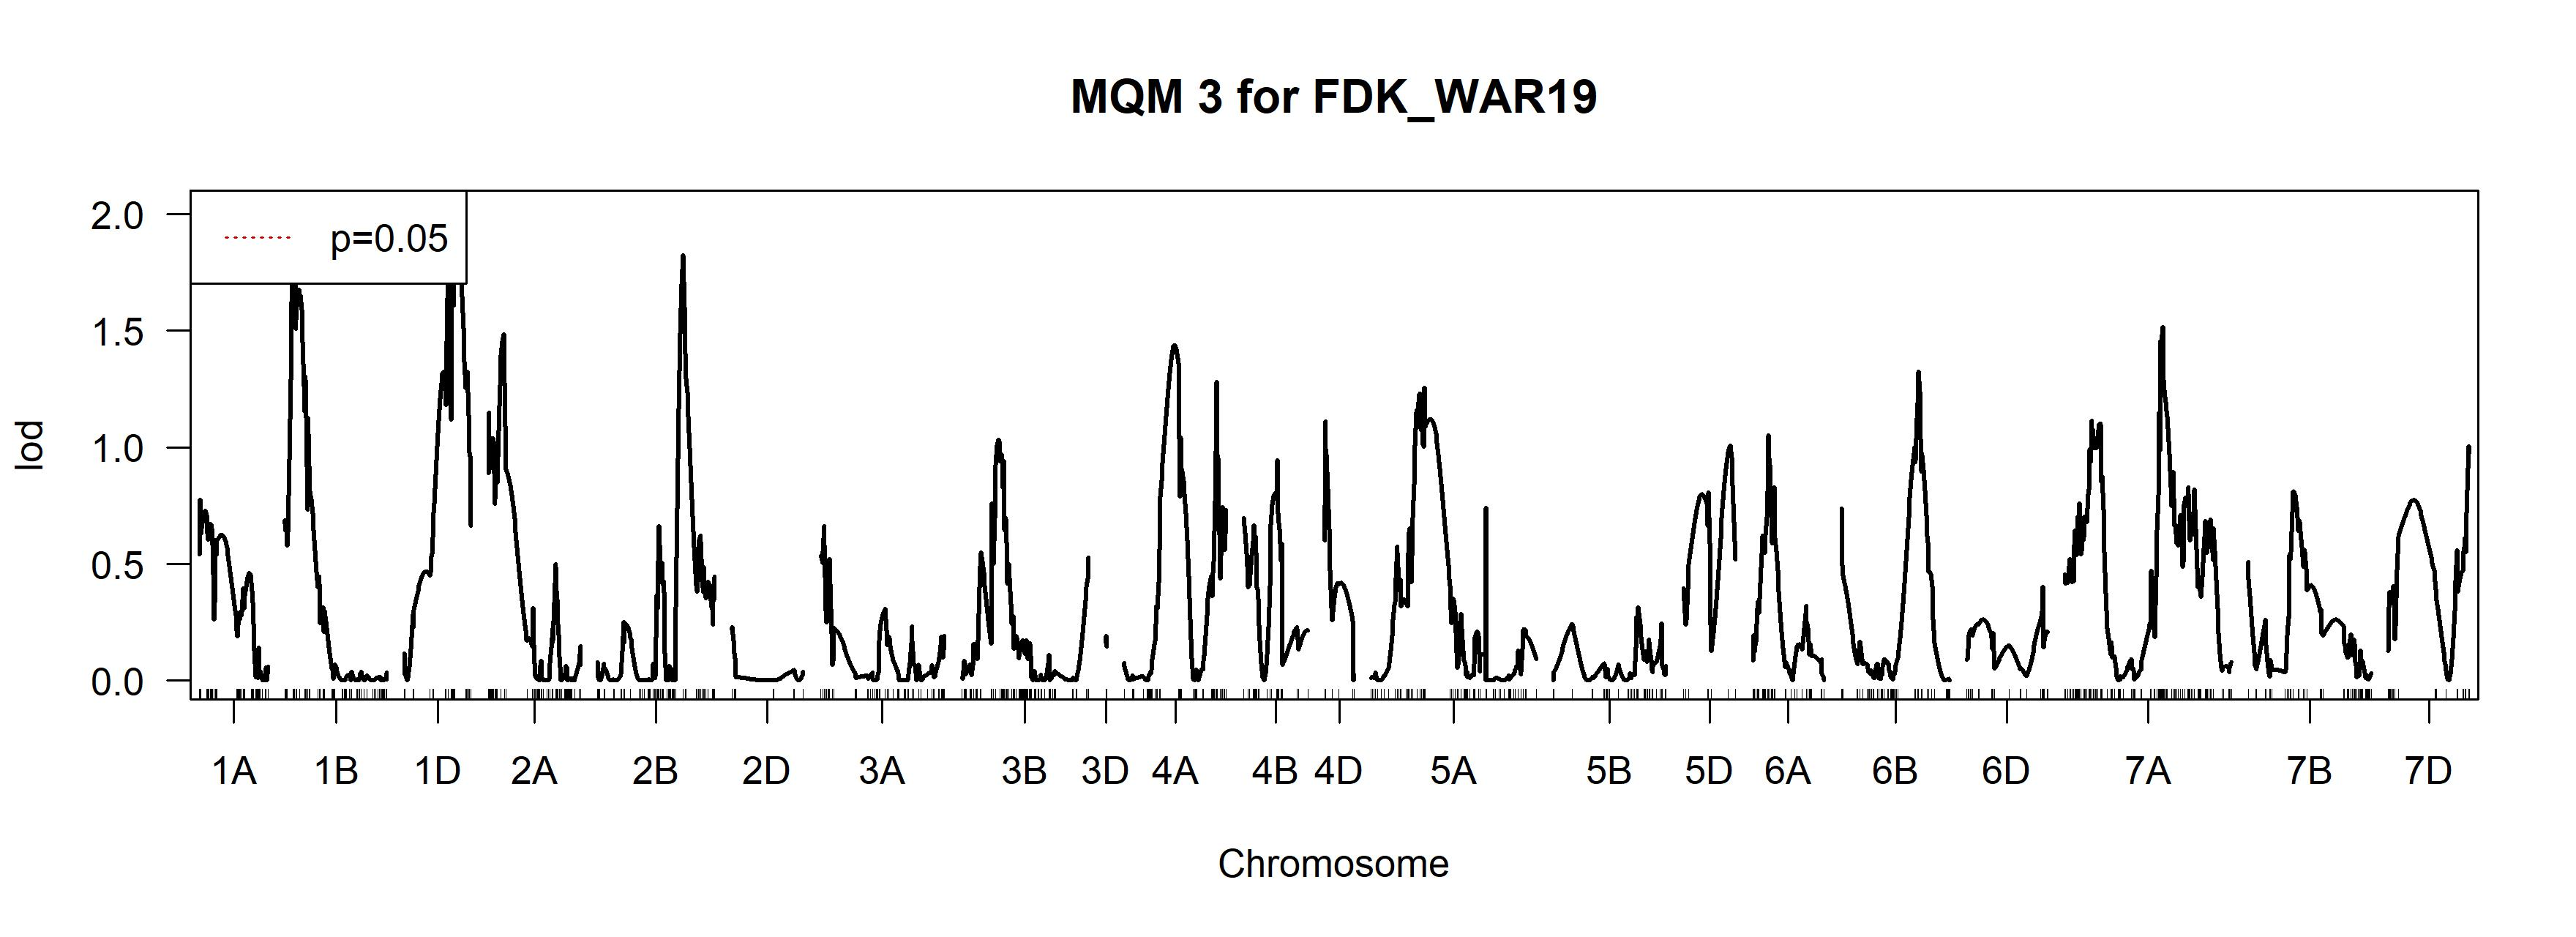
\includegraphics{Scan_MQM3_FDK_WAR19.jpg} \pagebreak

\subsection{Fusarium Damaged Kernels in Warsaw, VA -
2020}\label{fusarium-damaged-kernels-in-warsaw-va---2020}

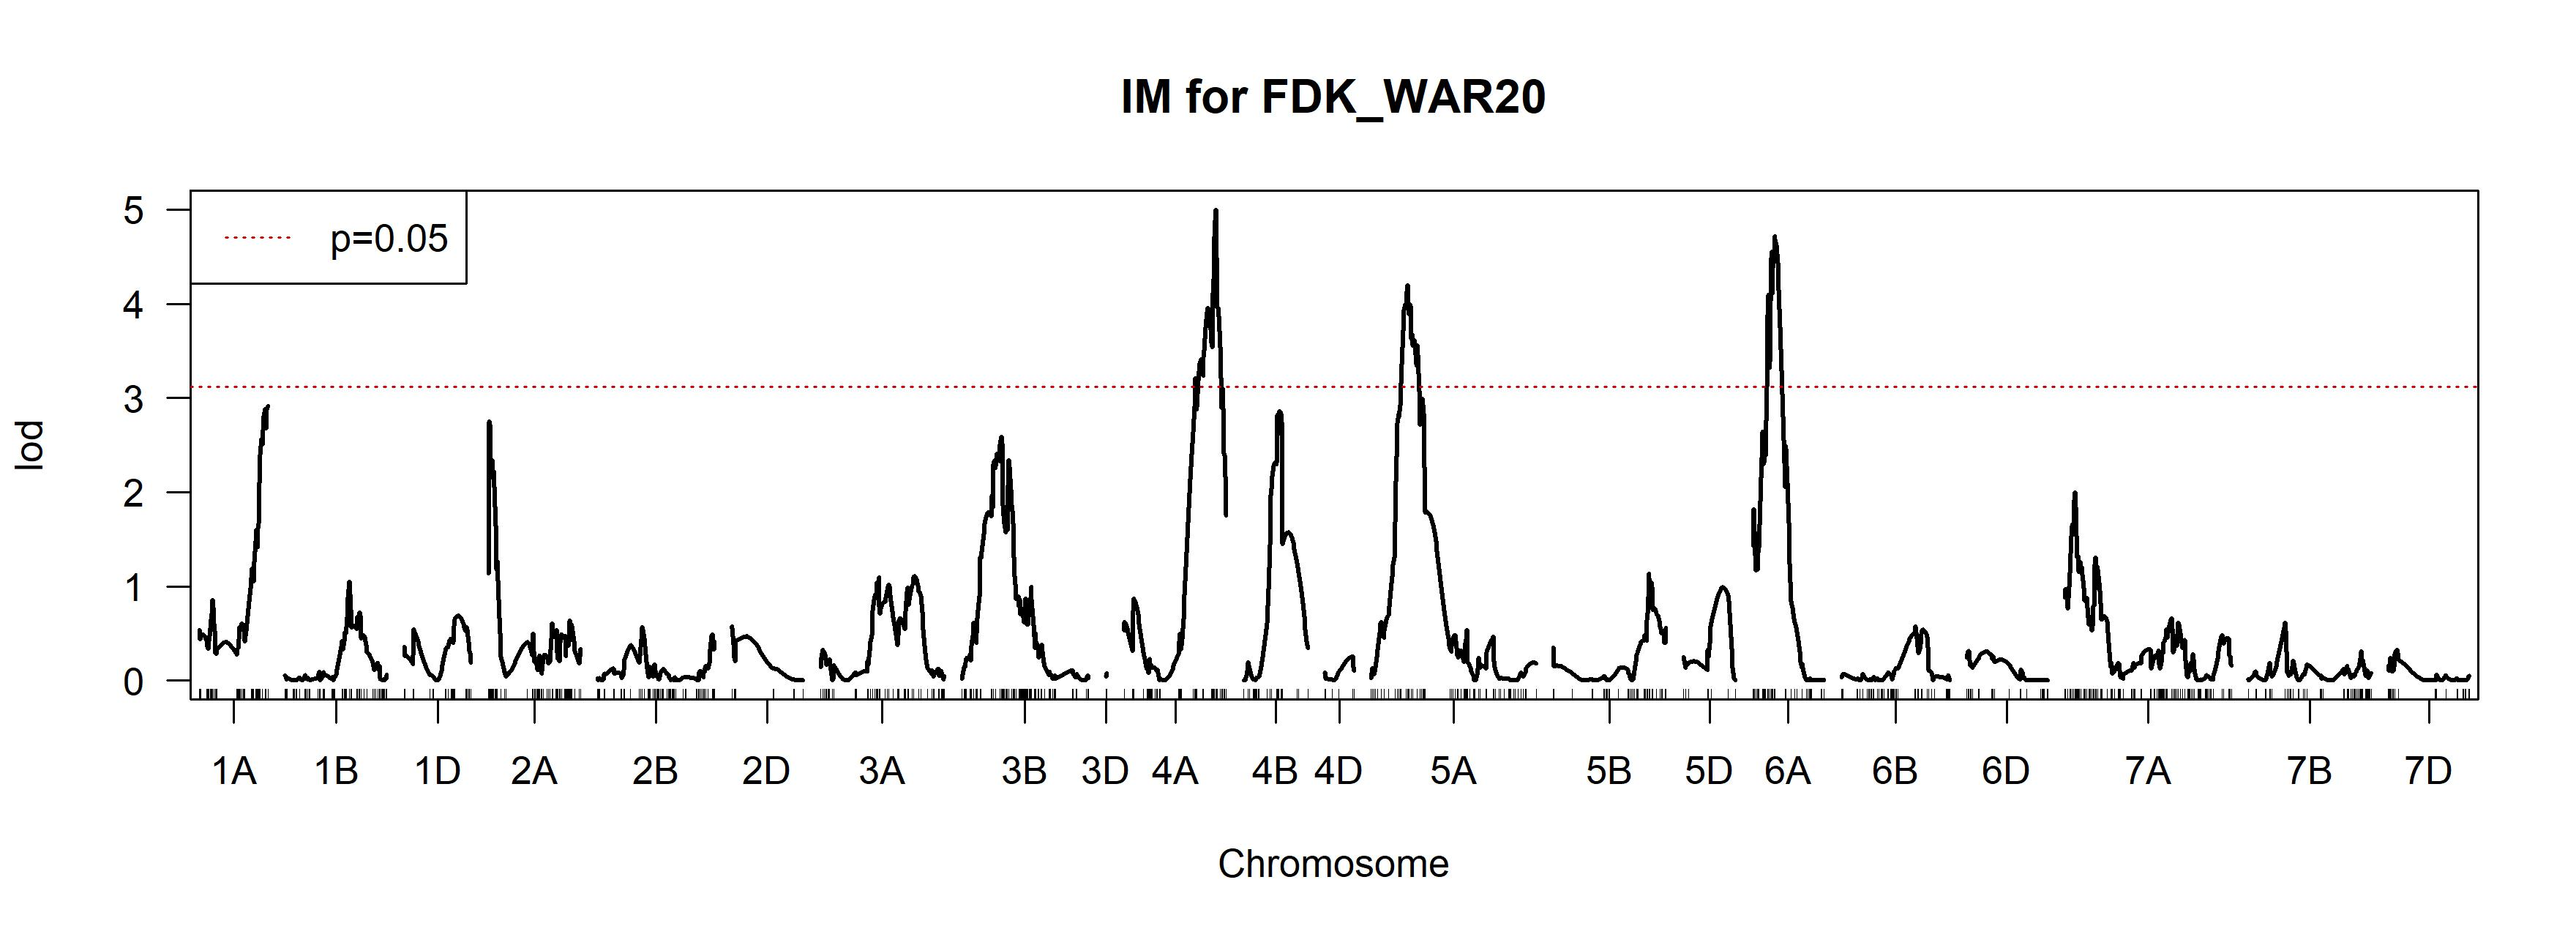
\includegraphics{Scan_IM_FDK_WAR20.jpg}
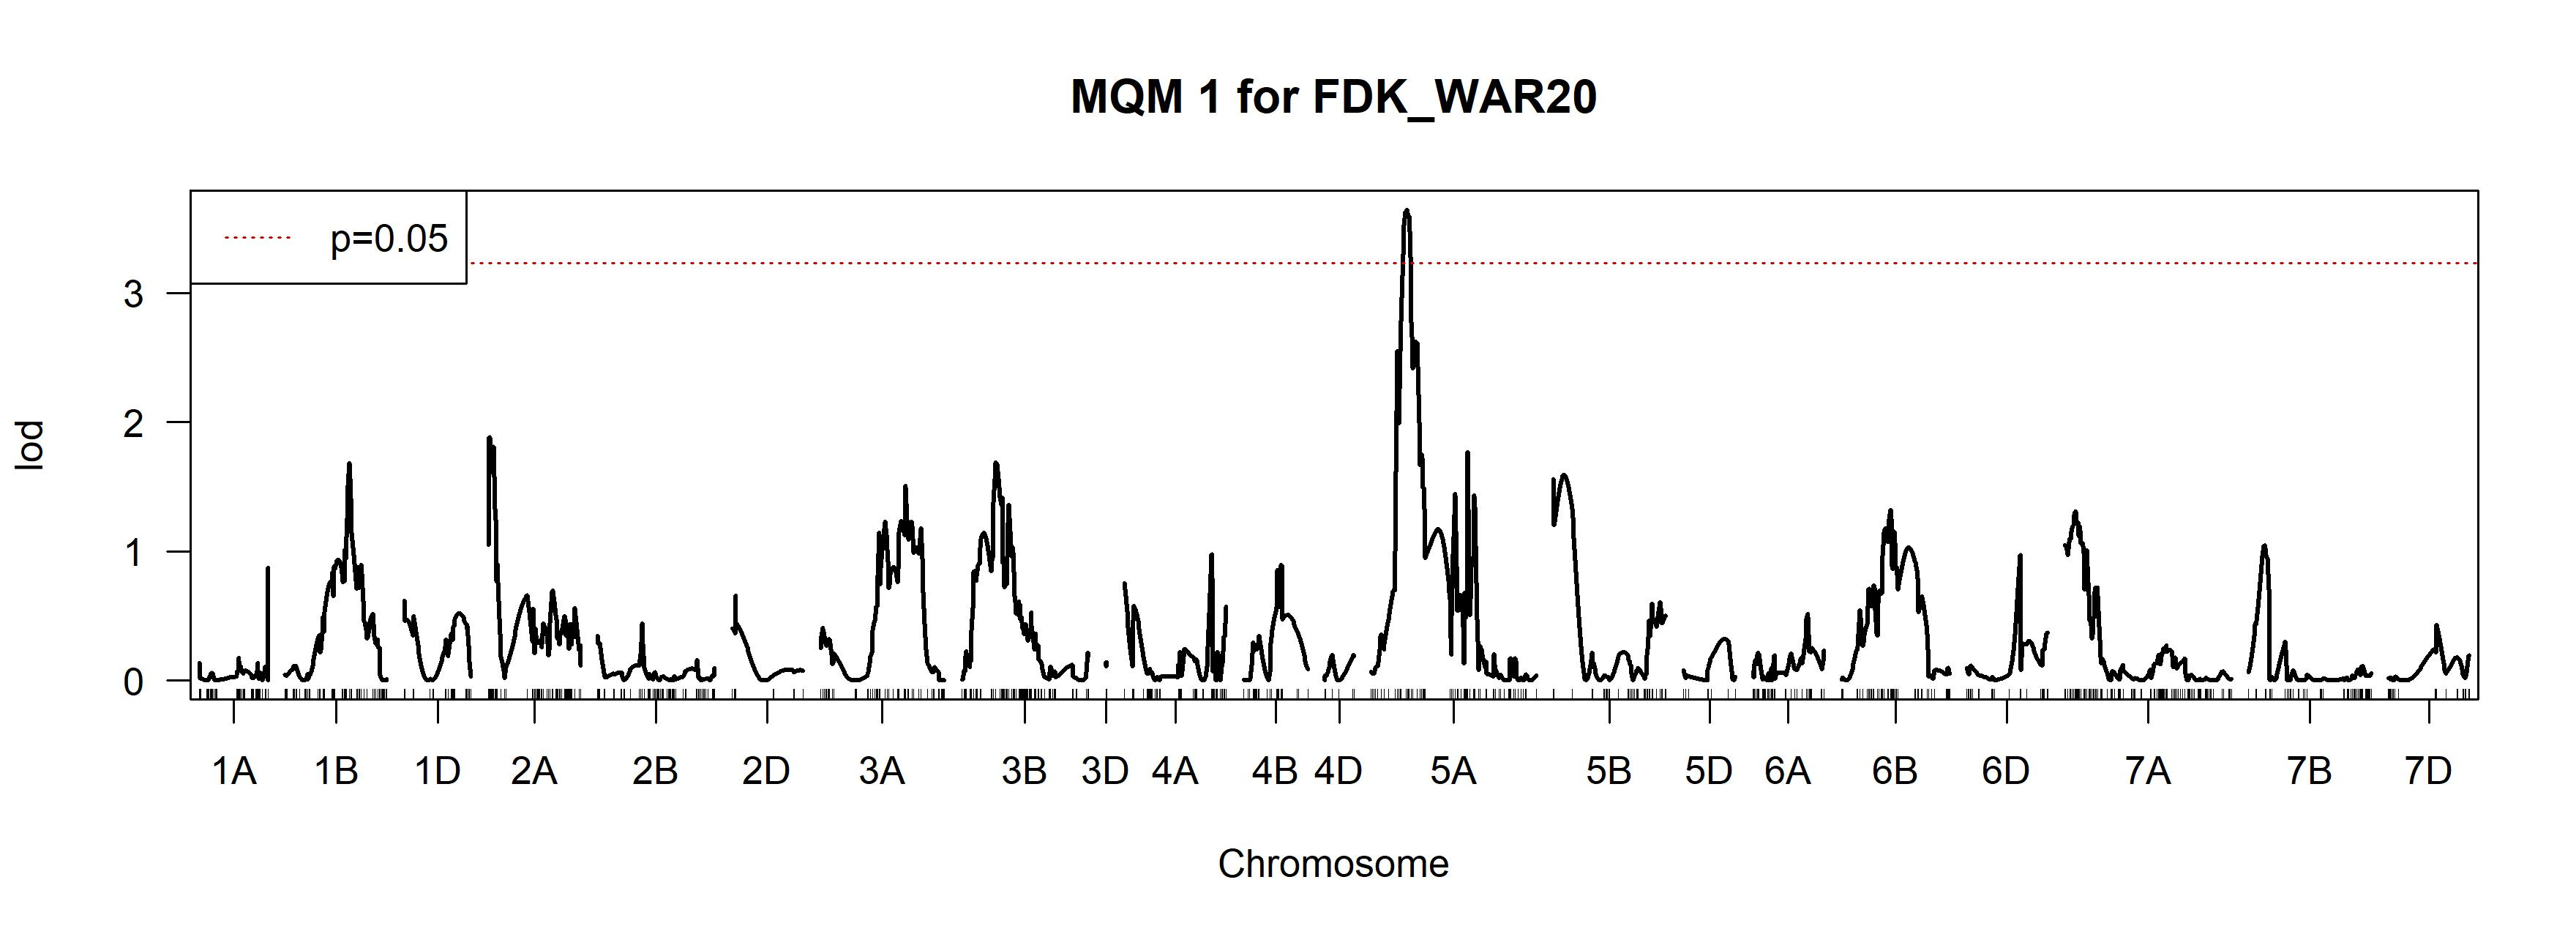
\includegraphics{Scan_MQM1_FDK_WAR20.jpg}
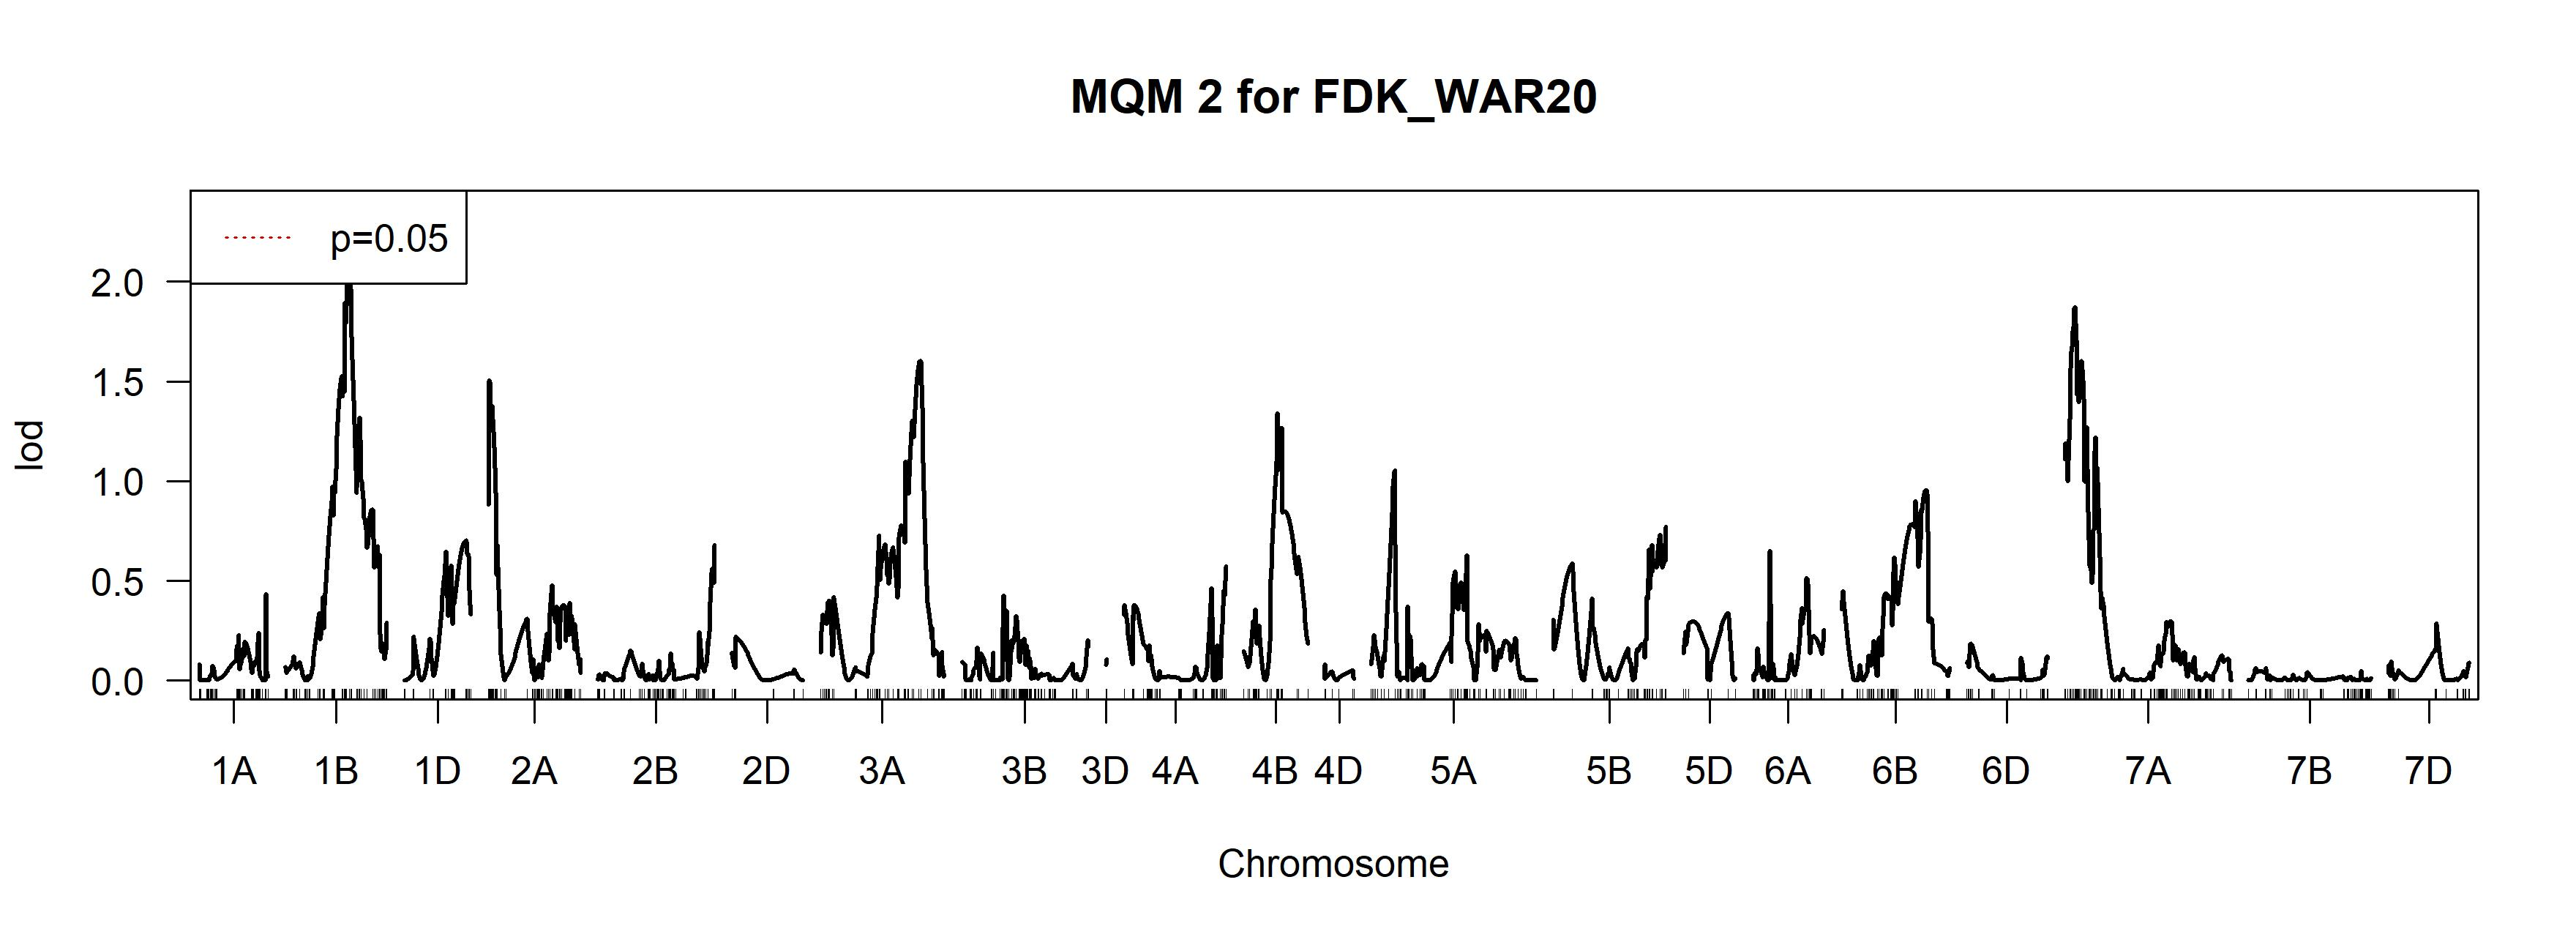
\includegraphics{Scan_MQM2_FDK_WAR20.jpg} \pagebreak

\subsection{Deoxynivalenol Content Across All
Environments}\label{deoxynivalenol-content-across-all-environments}

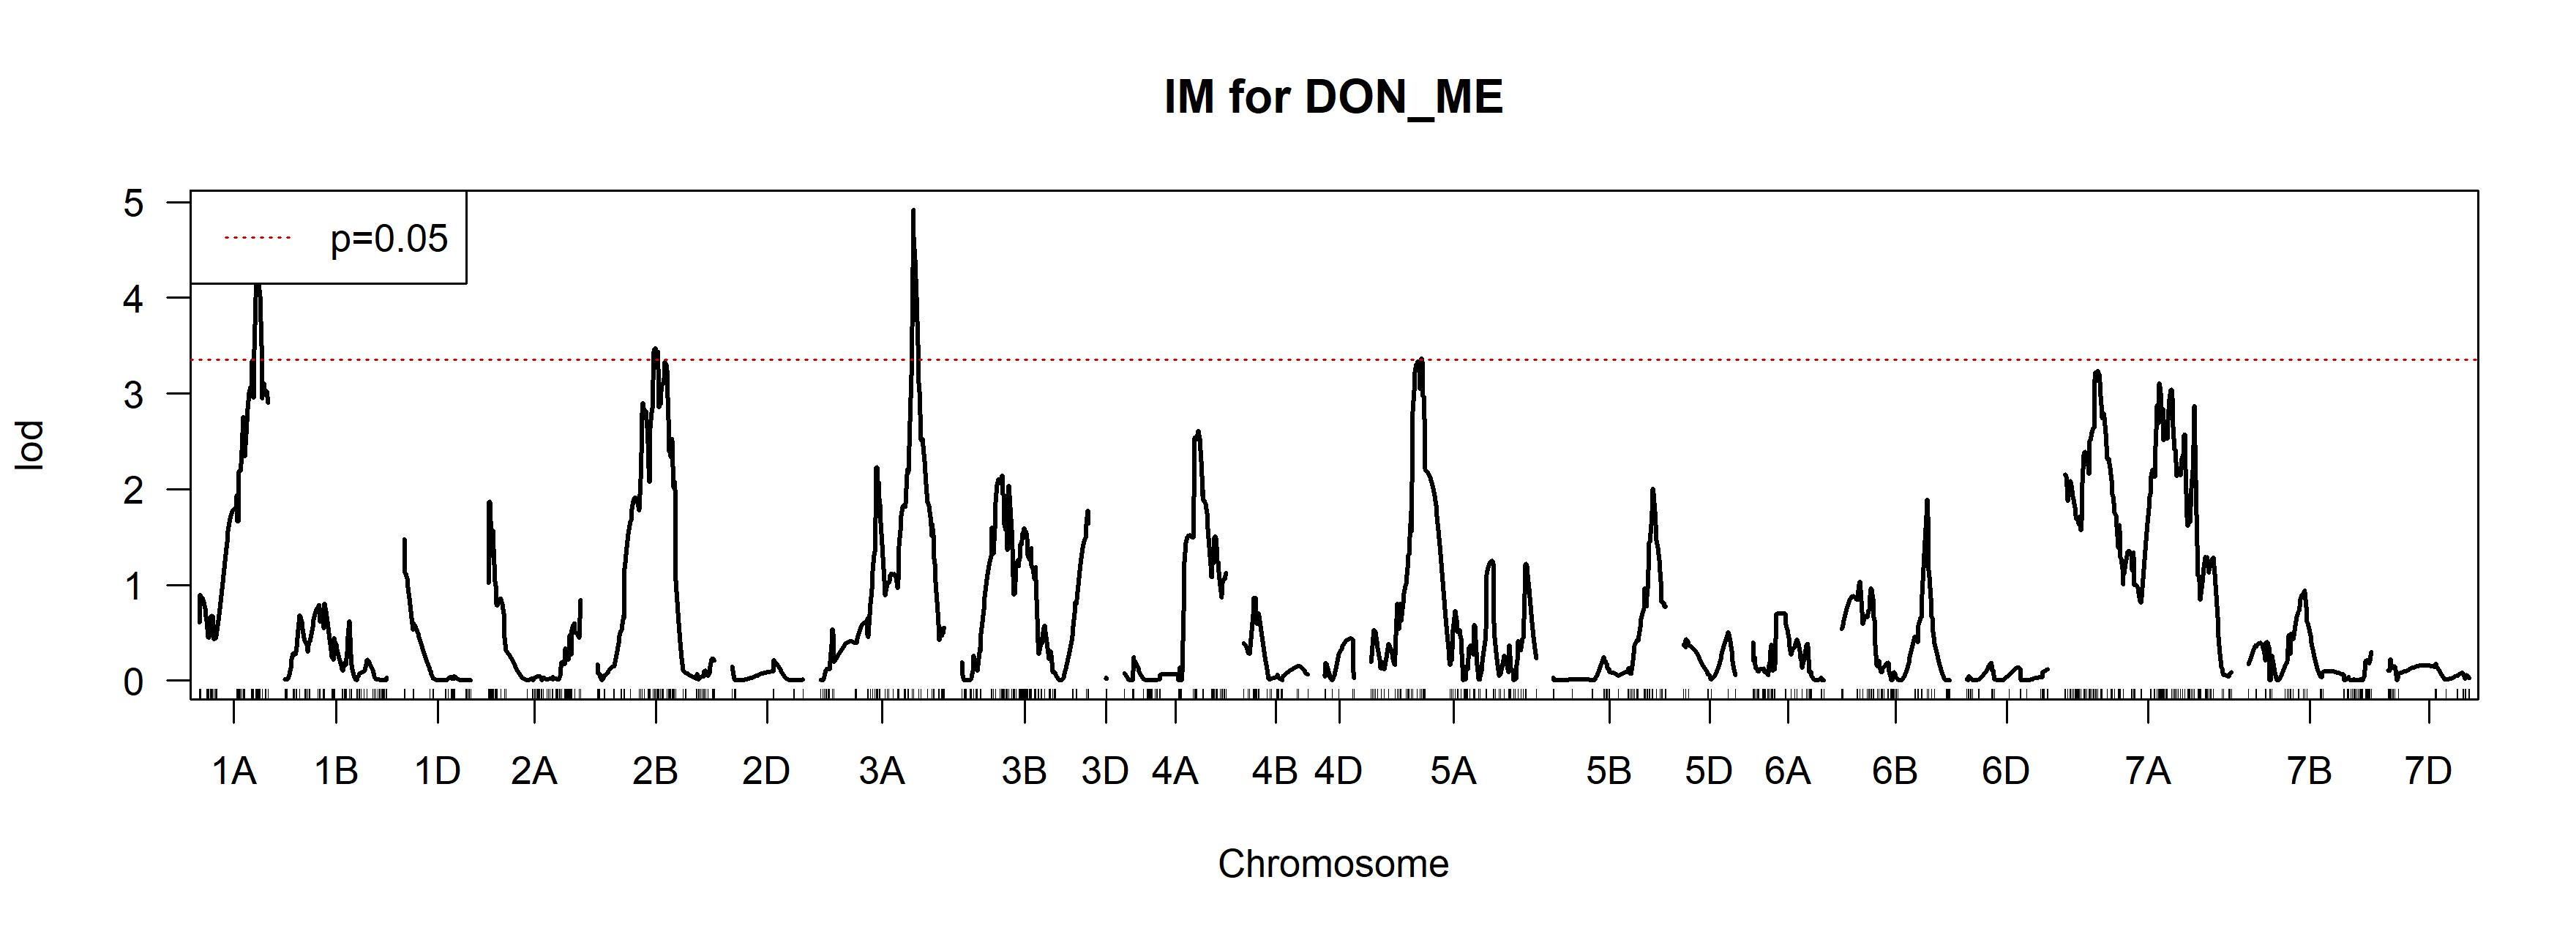
\includegraphics{Scan_IM_DON_ME.jpg}
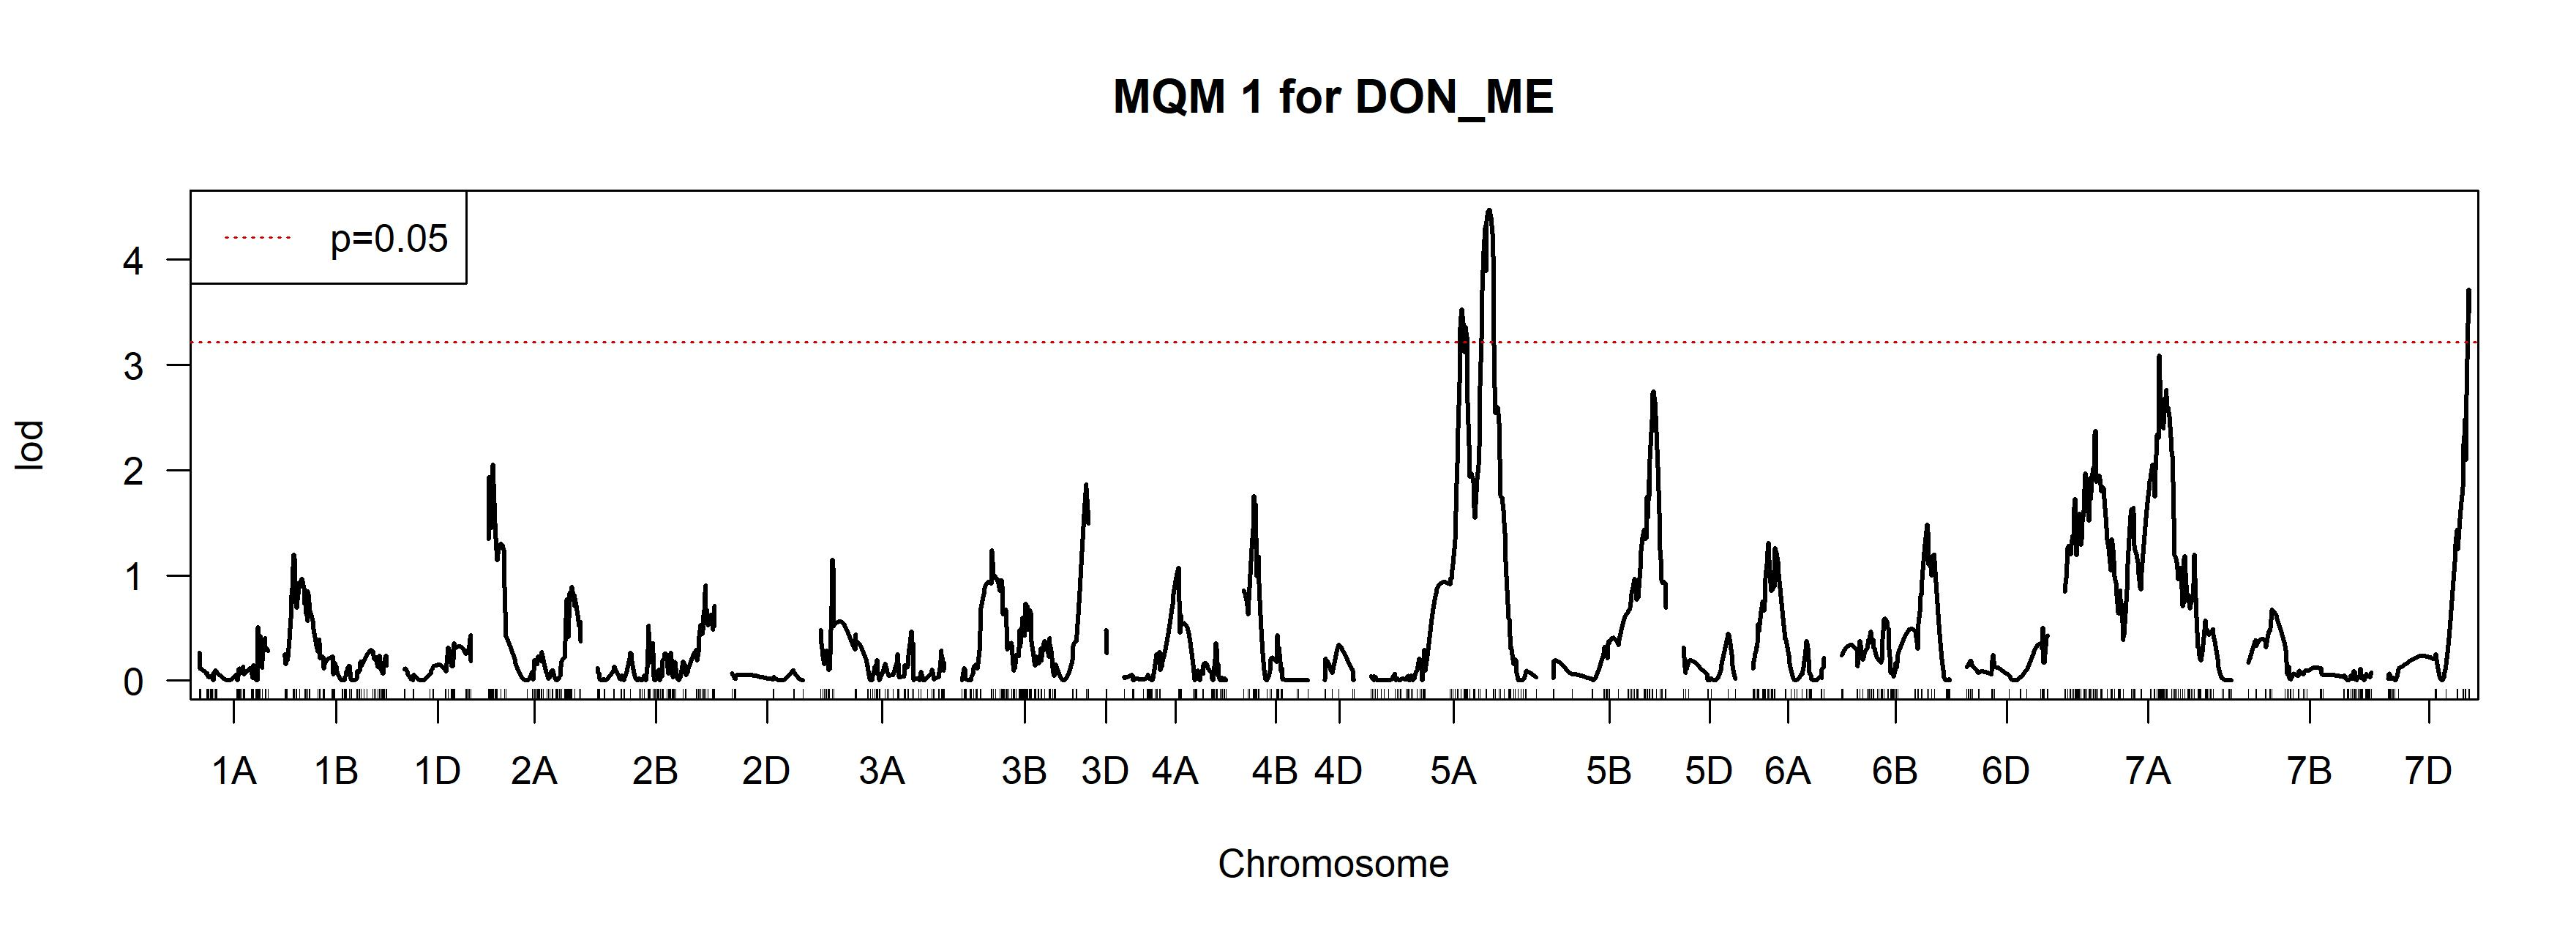
\includegraphics{Scan_MQM1_DON_ME.jpg}
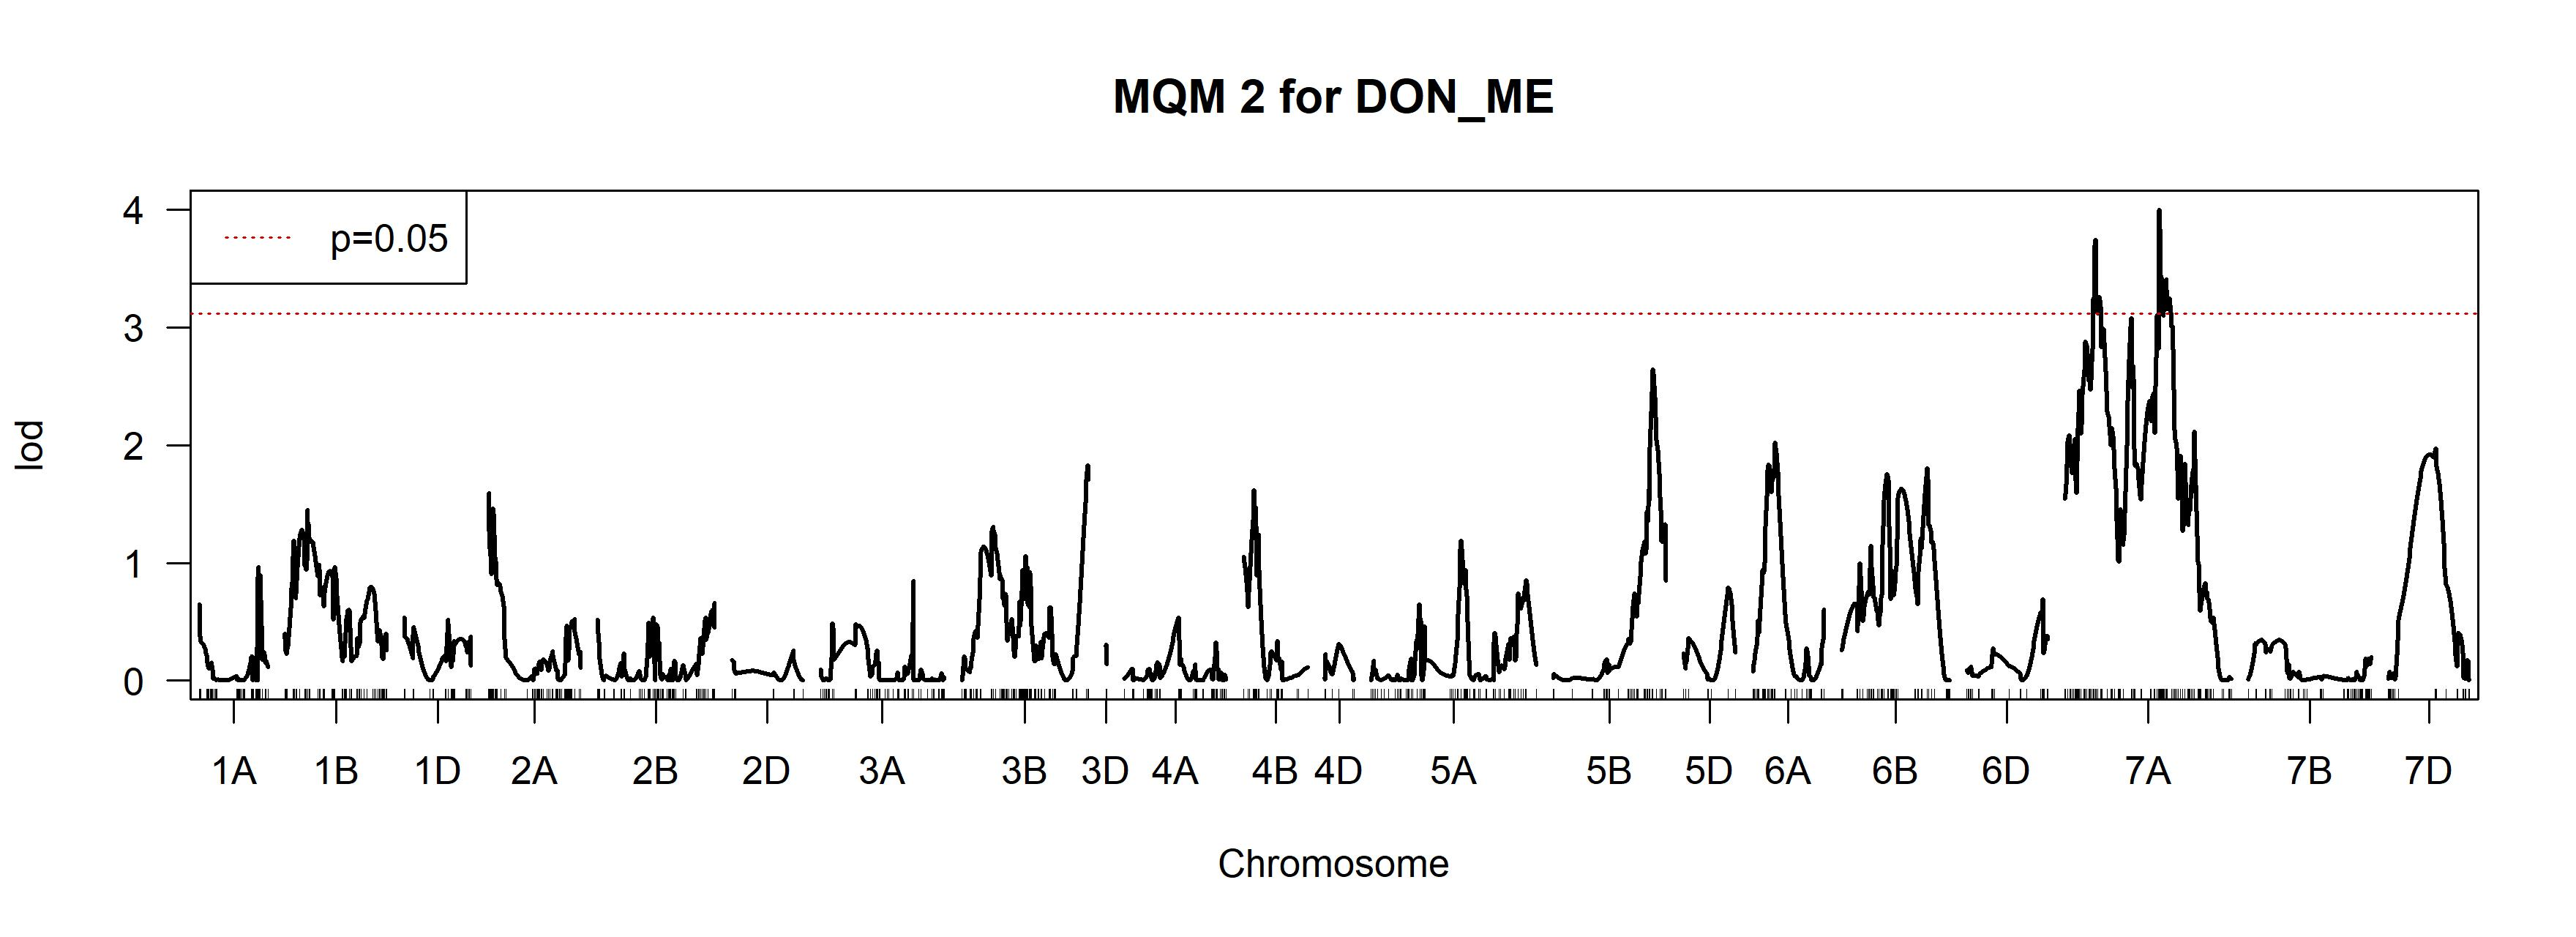
\includegraphics{Scan_MQM2_DON_ME.jpg}
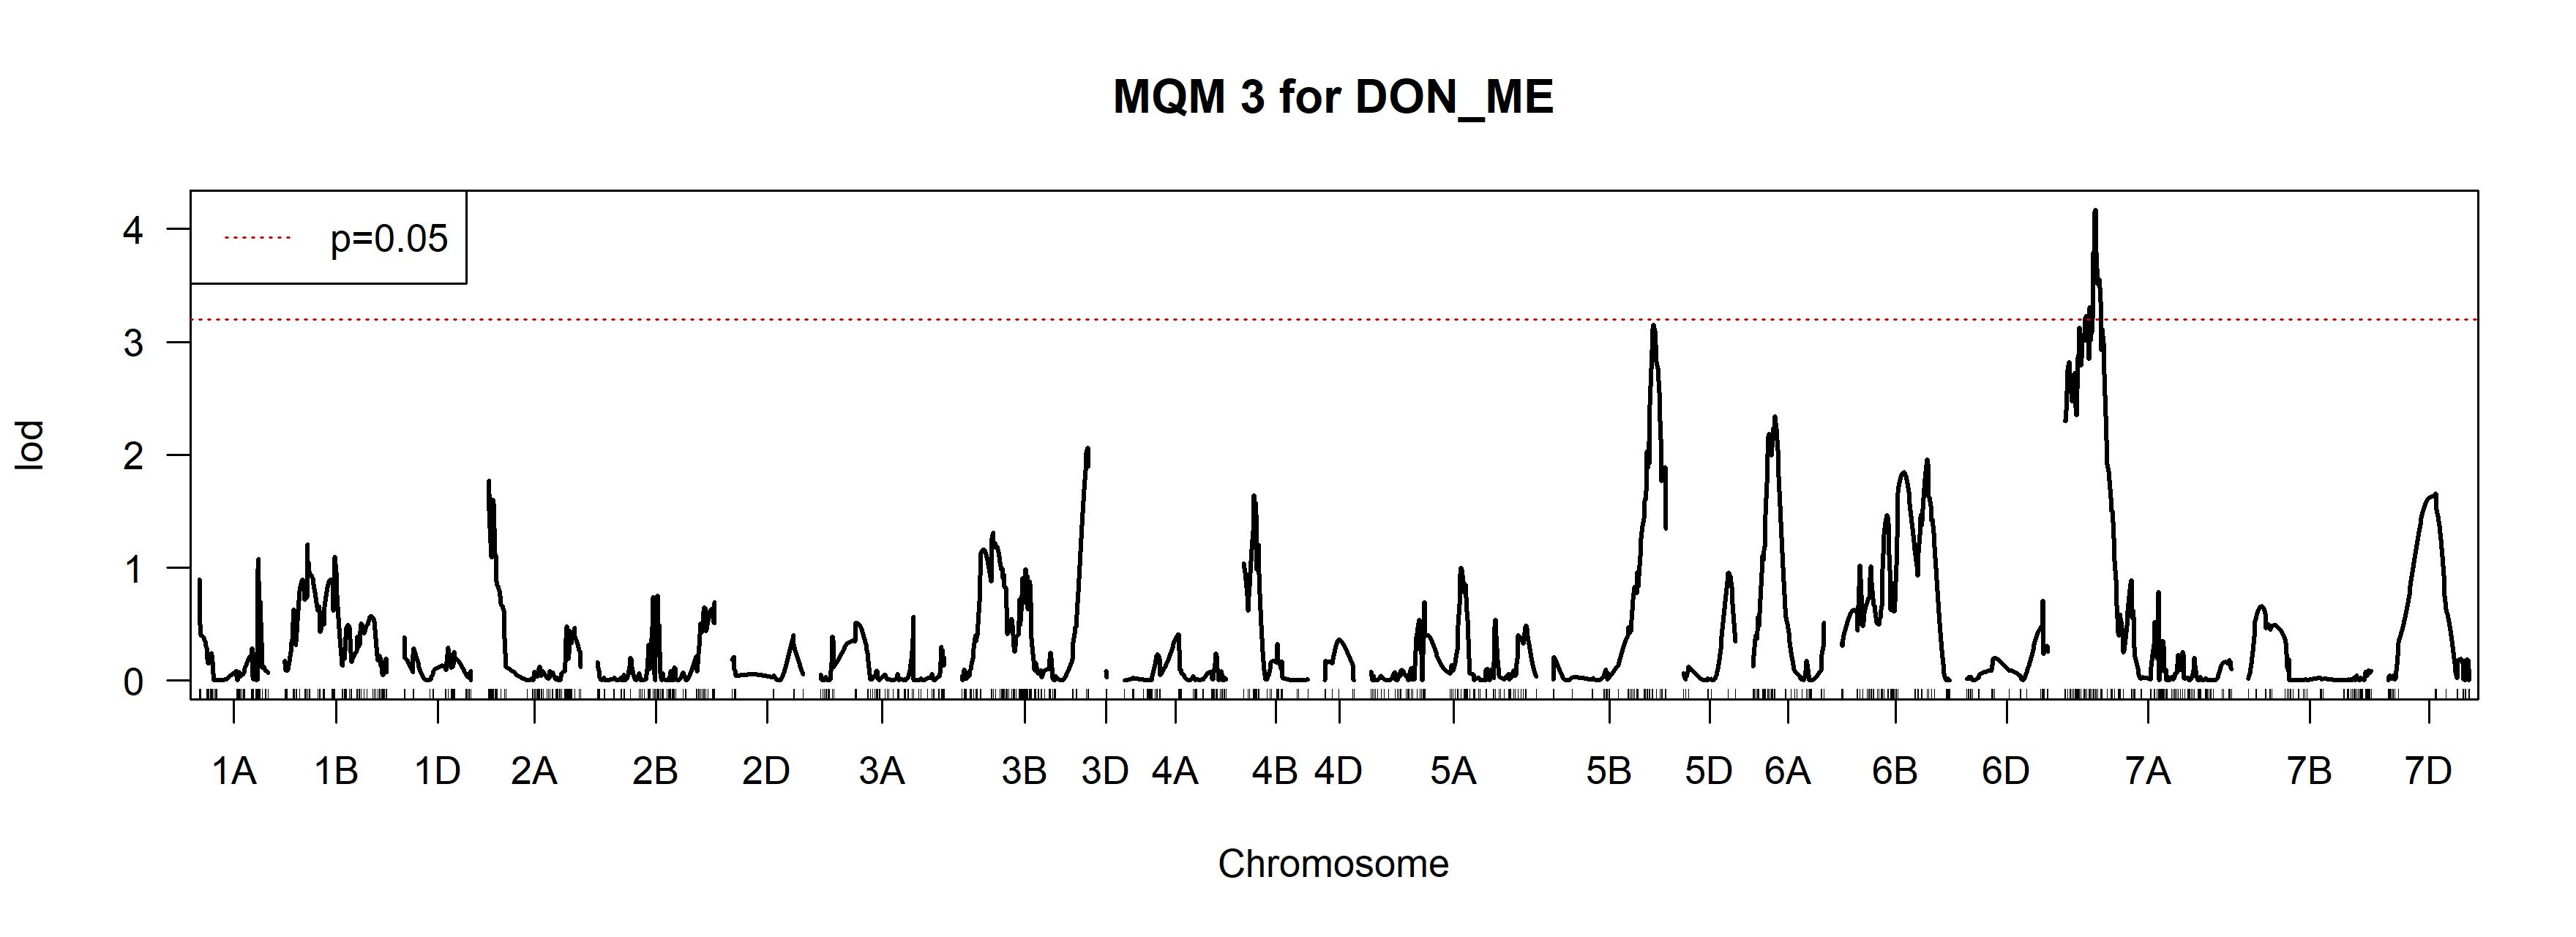
\includegraphics{Scan_MQM3_DON_ME.jpg}
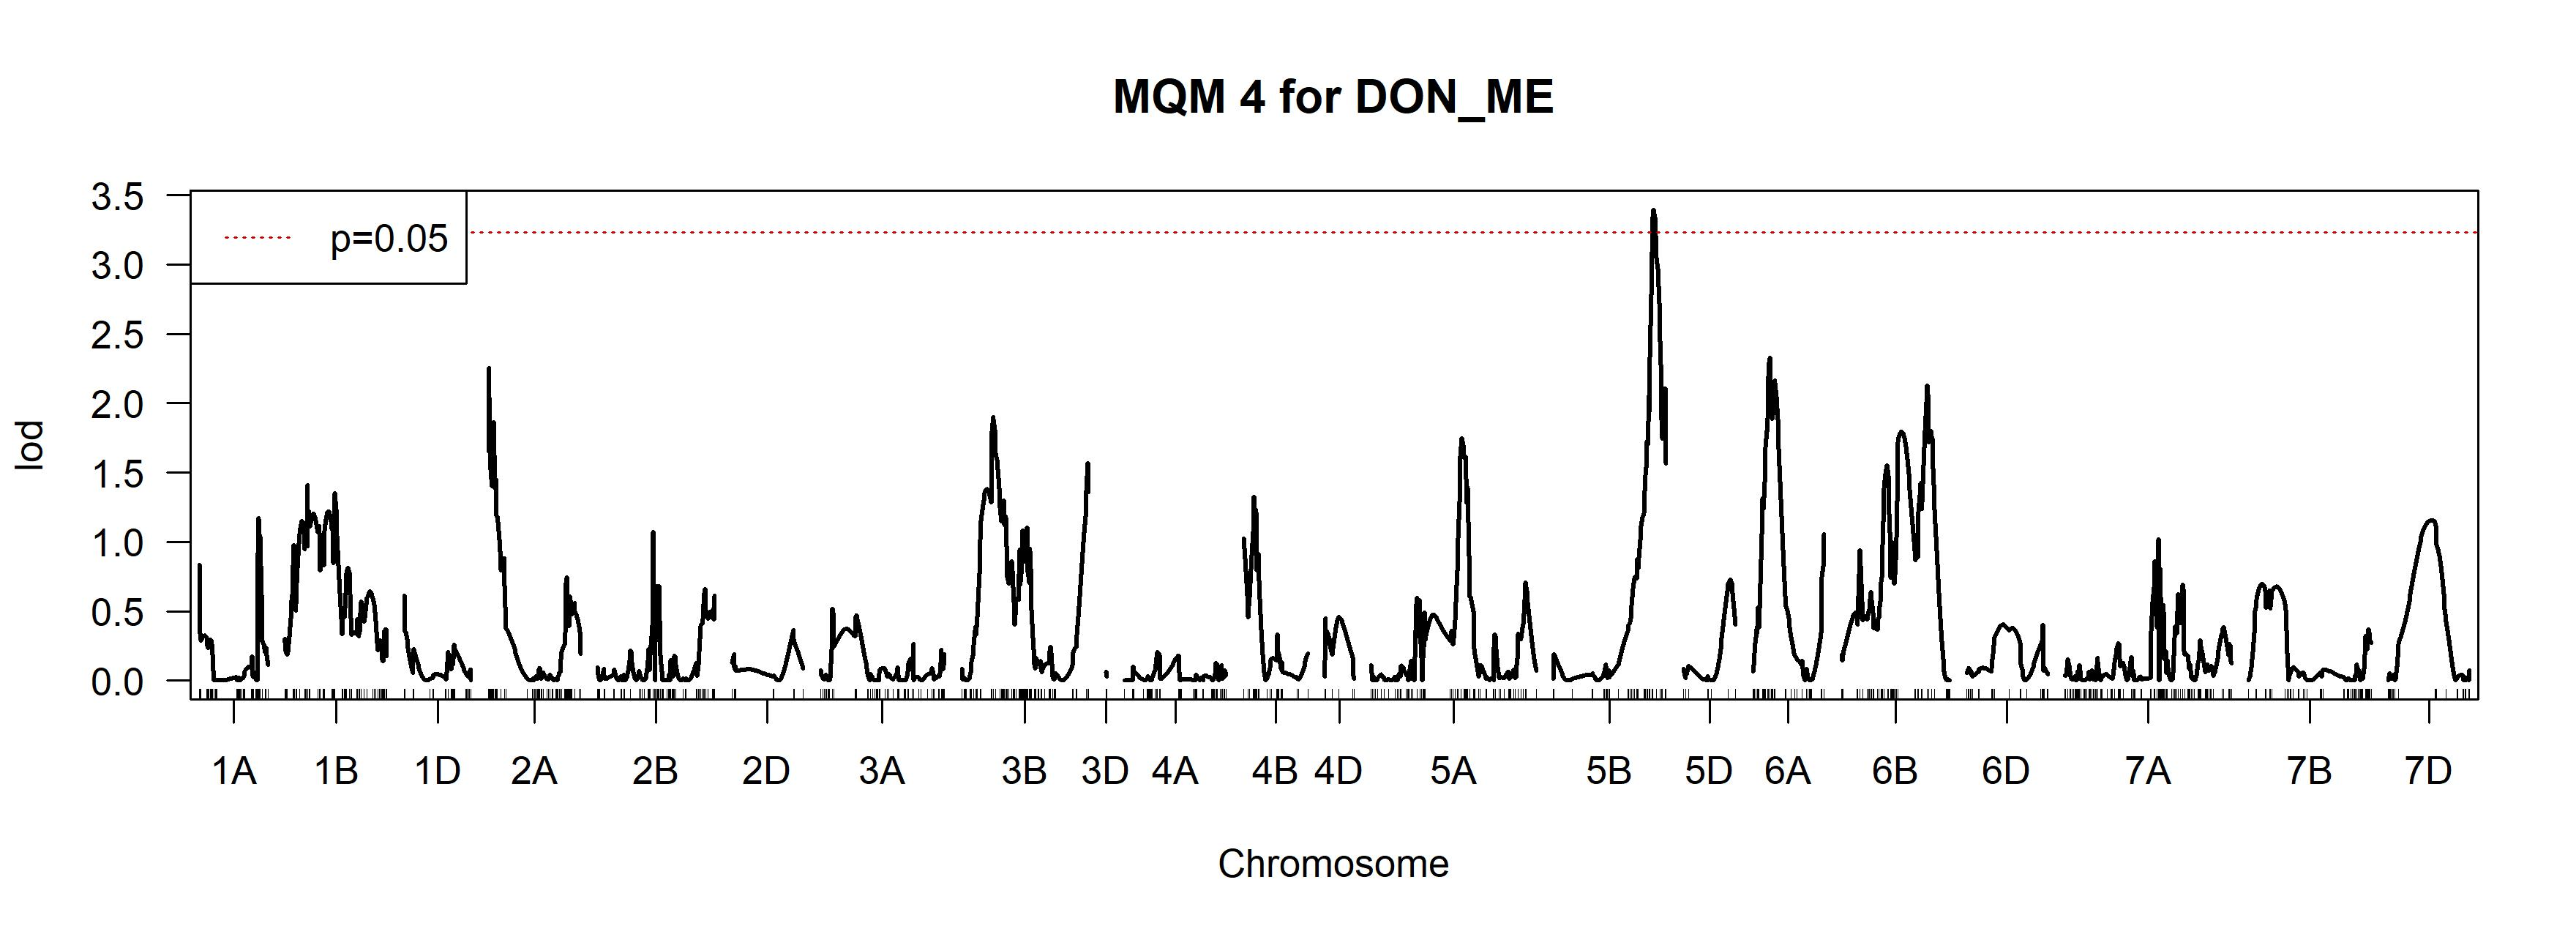
\includegraphics{Scan_MQM4_DON_ME.jpg}
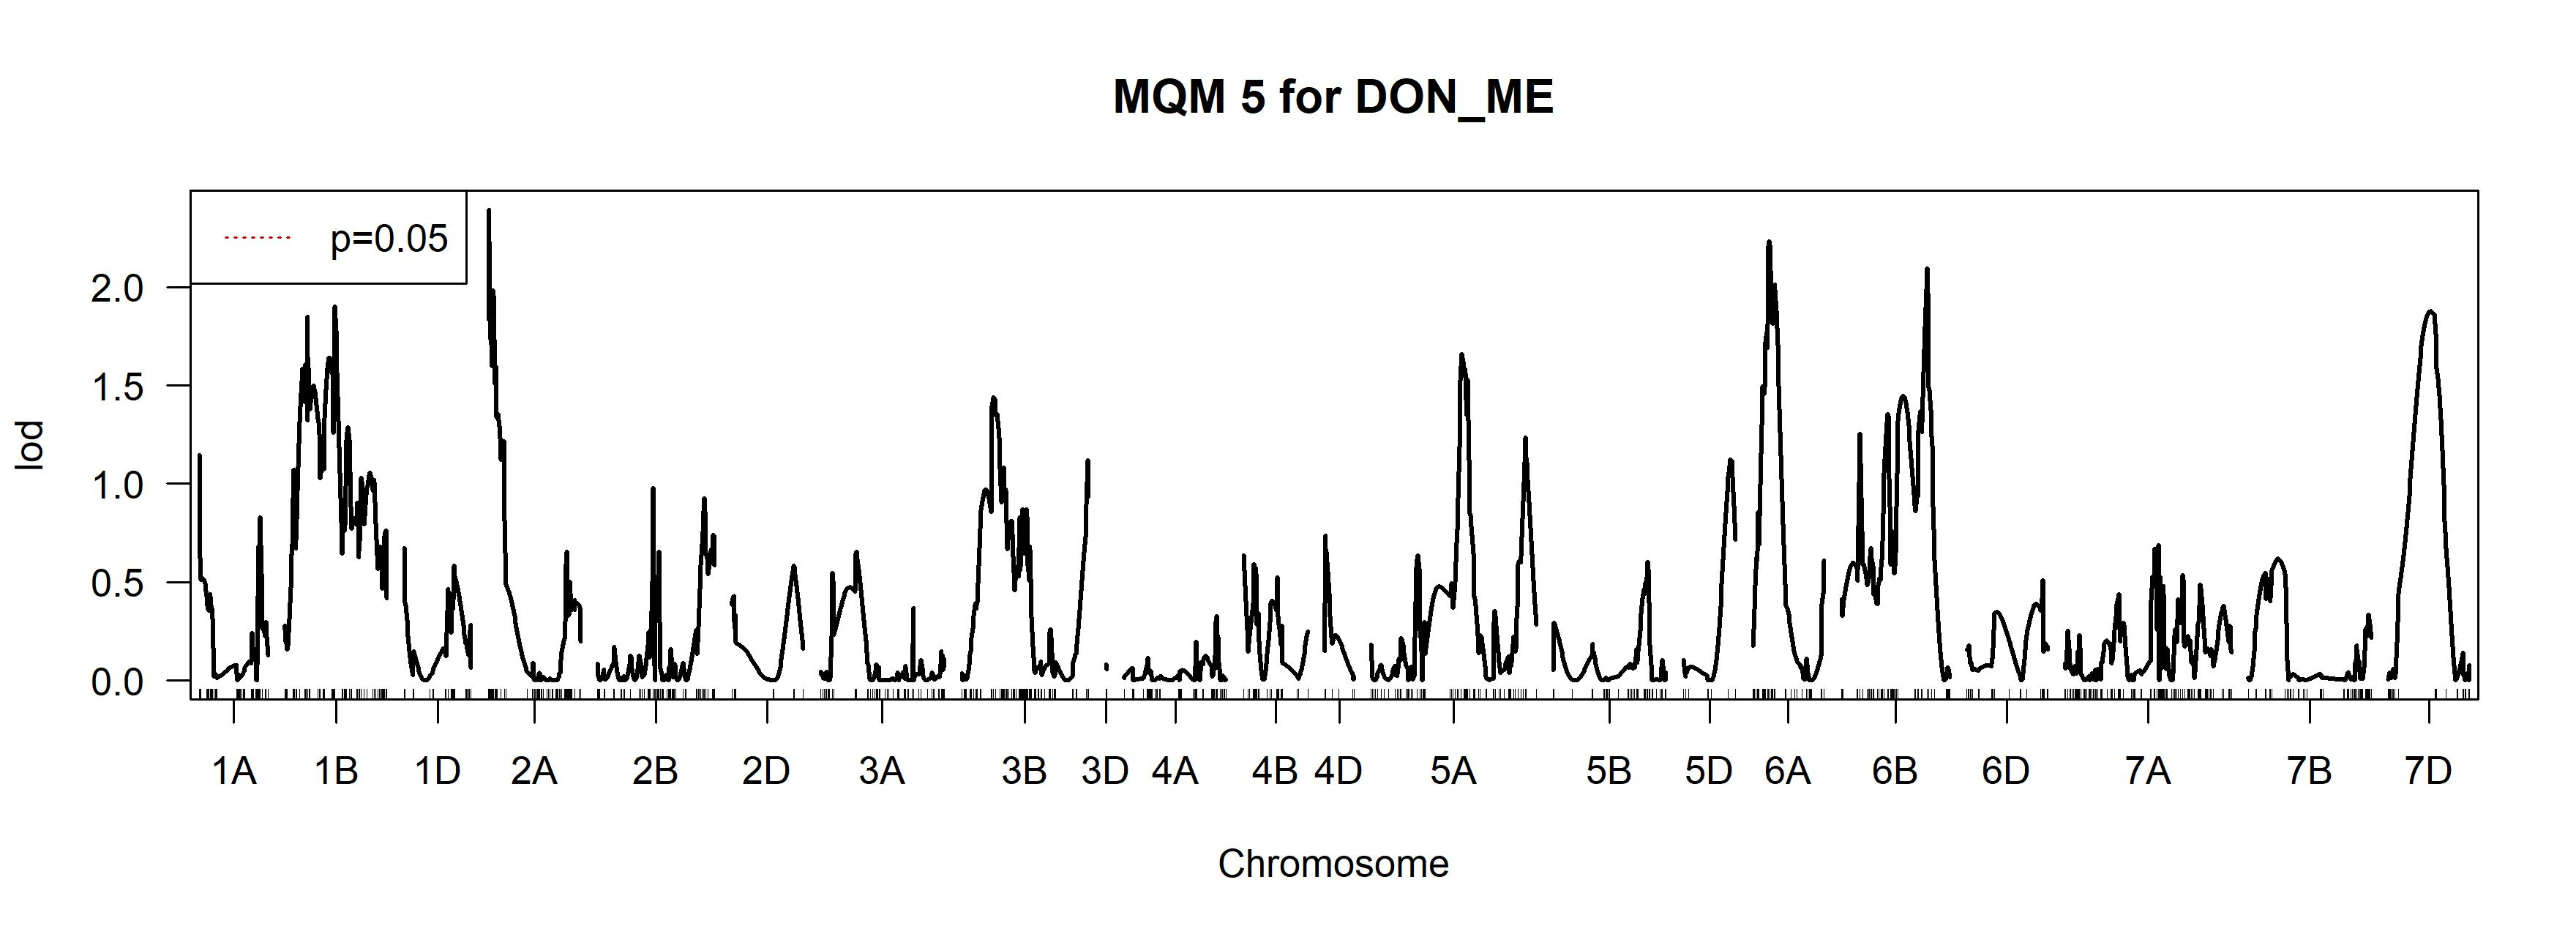
\includegraphics{Scan_MQM5_DON_ME.jpg} \pagebreak

\subsection{Deoxynivalenol Content in Kinston, NC -
2019}\label{deoxynivalenol-content-in-kinston-nc---2019}

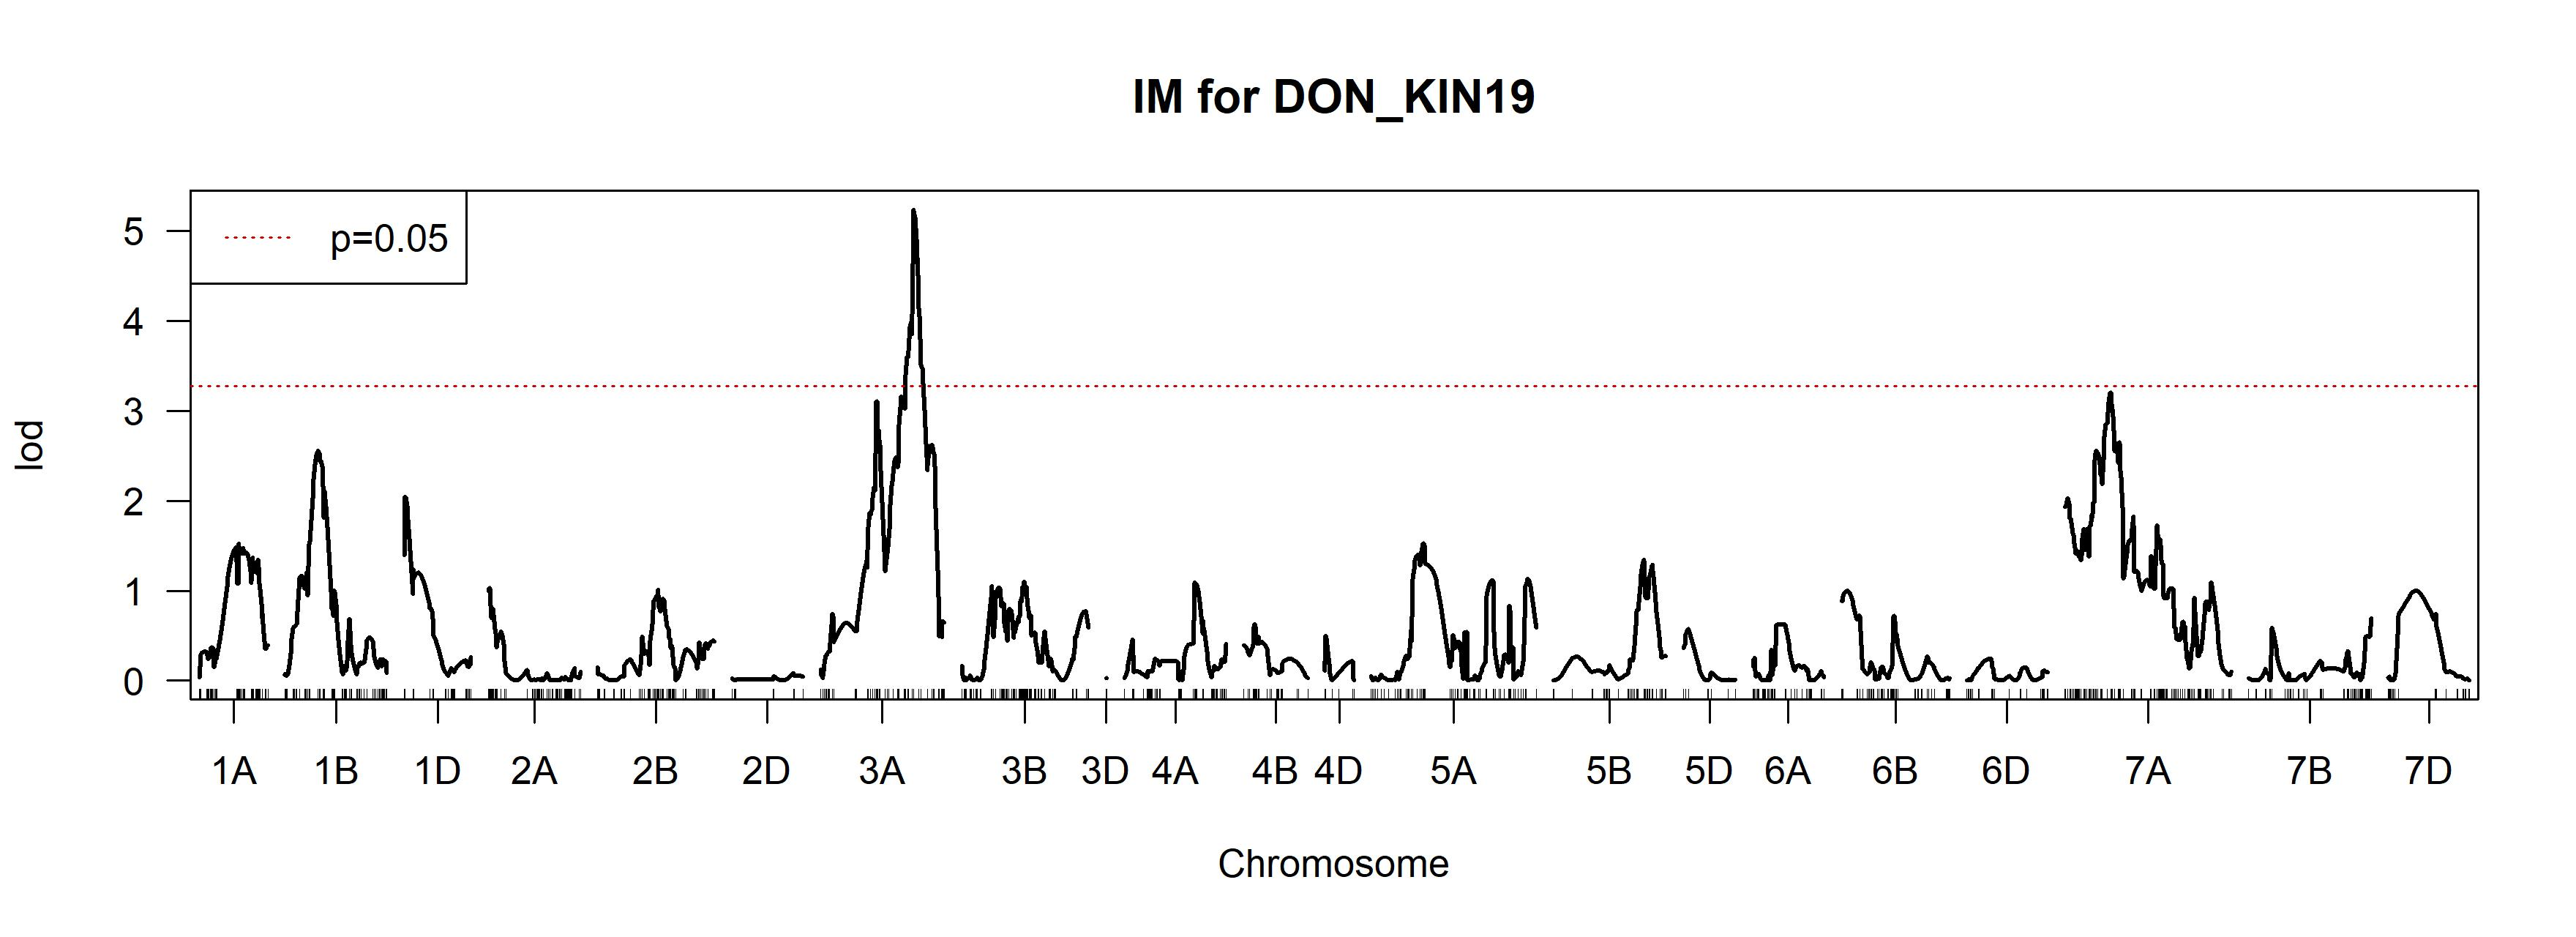
\includegraphics{Scan_IM_DON_KIN19.jpg}
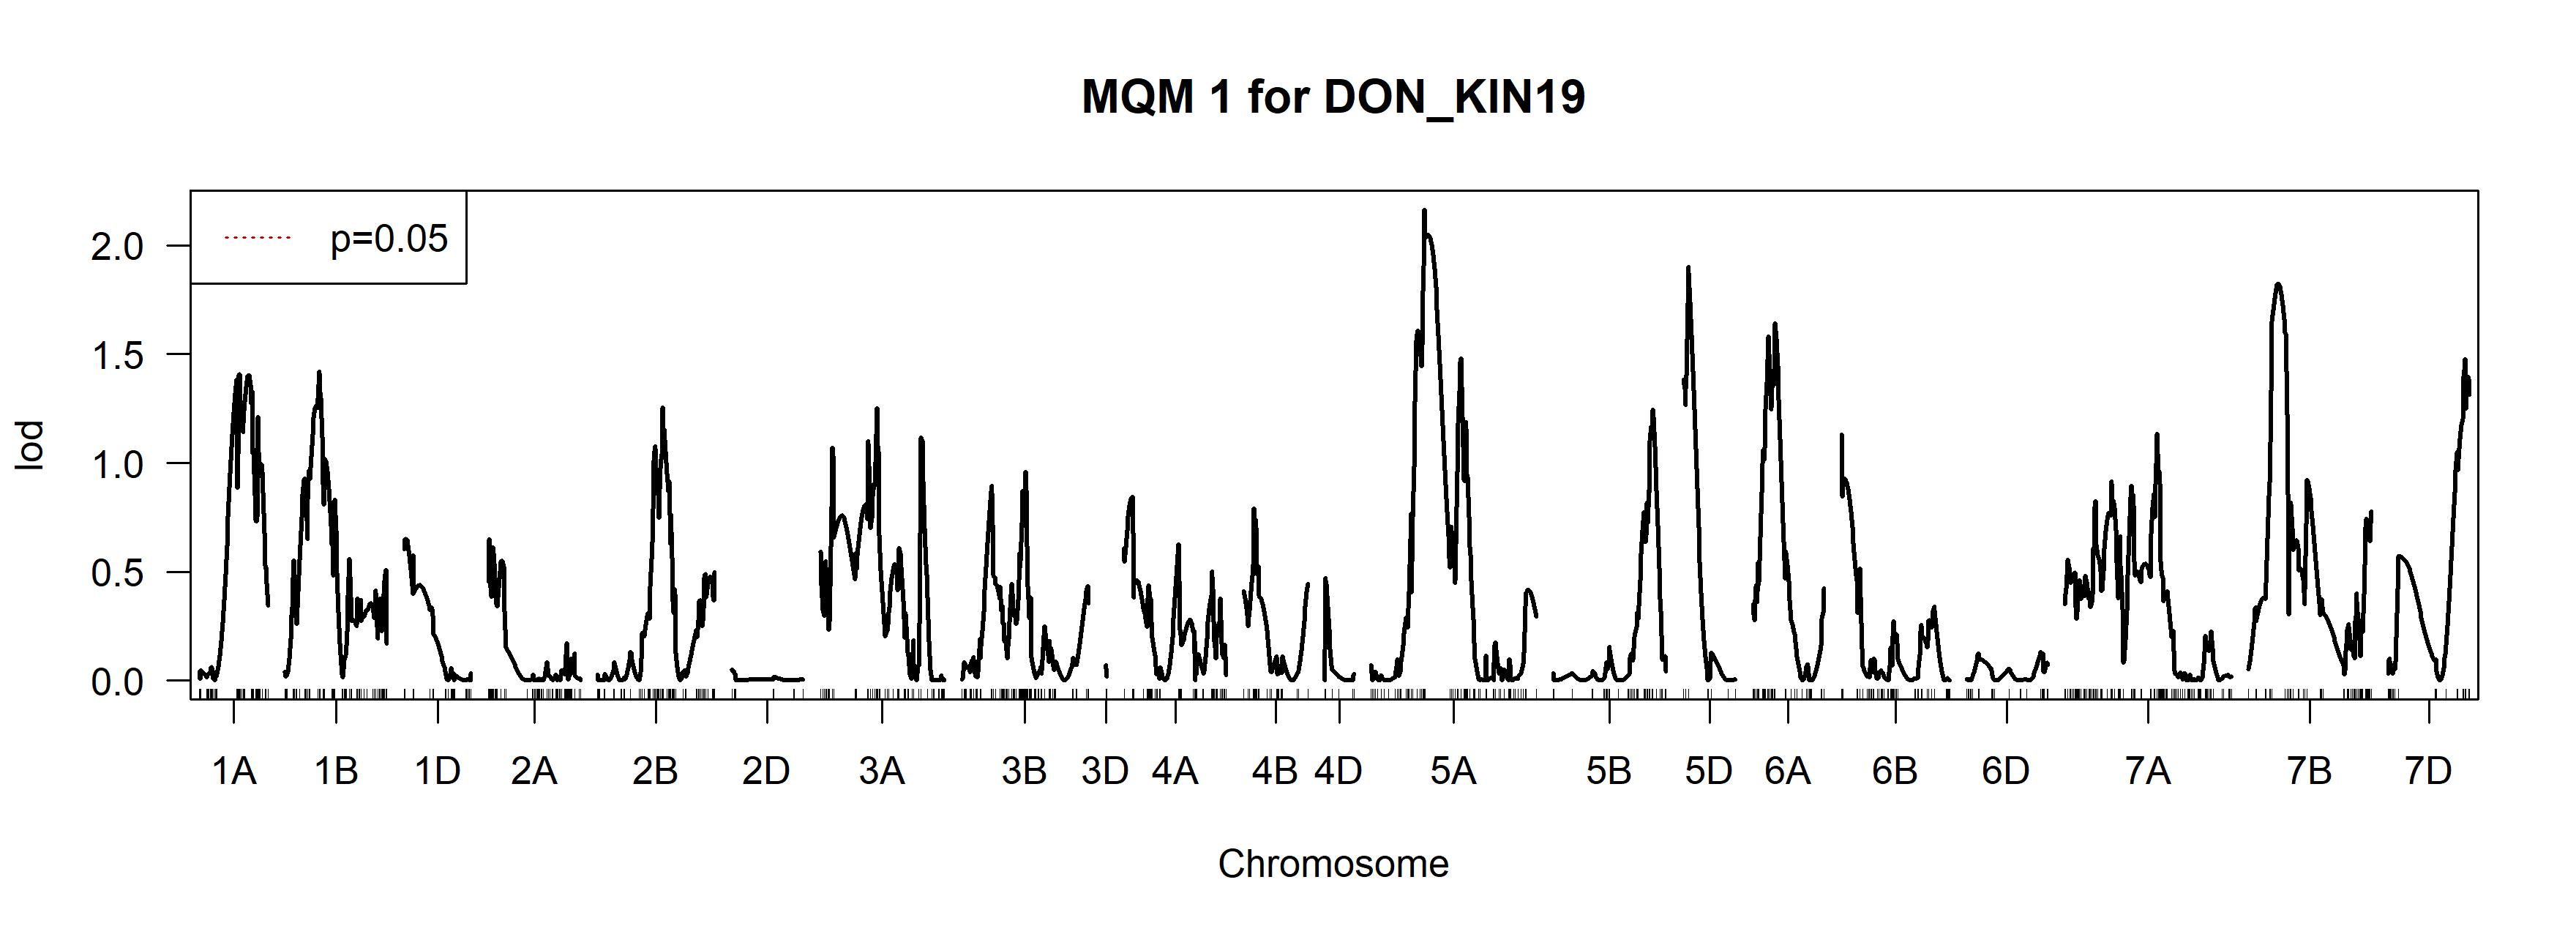
\includegraphics{Scan_MQM1_DON_KIN19.jpg} \pagebreak

\subsection{Deoxynivalenol Content in Kinston, NC -
2020}\label{deoxynivalenol-content-in-kinston-nc---2020}

\includegraphics{Scan_IM_DON_KIN20.jpg}
\includegraphics{Scan_MQM1_DON_KIN20.jpg}
\includegraphics{Scan_MQM2_DON_KIN20.jpg}
\includegraphics{Scan_MQM3_DON_KIN20.jpg} \pagebreak

\subsection{Deoxynivalenol Content in Raleigh, NC -
2019}\label{deoxynivalenol-content-in-raleigh-nc---2019}

\includegraphics{Scan_IM_DON_RAL19.jpg}
\includegraphics{Scan_MQM1_DON_RAL19.jpg}
\includegraphics{Scan_MQM2_DON_RAL19.jpg} \pagebreak

\subsection{Deoxynivalenol Content in Raleigh, NC -
2020}\label{deoxynivalenol-content-in-raleigh-nc---2020}

\includegraphics{Scan_IM_DON_RAL20.jpg}
\includegraphics{Scan_MQM1_DON_RAL20.jpg} \pagebreak

\subsection{Deoxynivalenol Content in Warsaw, VA -
2019}\label{deoxynivalenol-content-in-warsaw-va---2019}

\includegraphics{Scan_IM_DON_WAR19.jpg}
\includegraphics{Scan_MQM1_DON_WAR19.jpg}
\includegraphics{Scan_MQM2_DON_WAR19.jpg}
\includegraphics{Scan_MQM3_DON_WAR19.jpg} \pagebreak

\subsection{Deoxynivalenol Content in Warsaw, VA -
2020}\label{deoxynivalenol-content-in-warsaw-va---2020}

\includegraphics{Scan_IM_DON_WAR20.jpg}
\includegraphics{Scan_MQM1_DON_WAR20.jpg} \pagebreak

\end{document}
